\documentclass[12pt,a4paper]{report}

% === 中文支持 ===
\usepackage[UTF8]{ctex}
\setCJKmainfont{PingFang SC}
\setCJKsansfont{PingFang SC}
\setCJKmonofont{PingFang SC}

% === 页面布局 ===
\usepackage[top=2.5cm, bottom=2.5cm, left=3cm, right=2.5cm]{geometry}

% === 基础宏包 ===
\usepackage{amsmath,amssymb}
\usepackage{graphicx}
\usepackage{booktabs}
\usepackage{longtable}
\usepackage{hyperref}
\usepackage{xcolor}
\usepackage{listings}
\usepackage{fancyhdr}
\usepackage{titlesec}
\usepackage{enumitem}
\usepackage{caption}
\usepackage{float}

% === 超链接 ===
\hypersetup{
    colorlinks=true,
    linkcolor=blue!70!black,
    citecolor=green!50!black,
    urlcolor=blue!60!black
}

% === 代码高亮 ===
\lstset{
    basicstyle=\small\ttfamily,
    breaklines=true,
    frame=single,
    backgroundcolor=\color{gray!8},
    keywordstyle=\color{blue!80!black}\bfseries,
    commentstyle=\color{green!50!black},
    stringstyle=\color{red!70!black},
    showstringspaces=false,
    tabsize=4,
    xleftmargin=1em,
    xrightmargin=1em,
    aboveskip=1em,
    belowskip=1em
}

% === 页眉页脚 ===
\pagestyle{fancy}
\fancyhf{}
\fancyhead[L]{\leftmark}
\fancyhead[R]{\thepage}
\renewcommand{\headrulewidth}{0.4pt}

% === 章节标题格式 ===
\titleformat{\chapter}[display]
  {\normalfont\Huge\bfseries}
  {第\,\thechapter\,章}{12pt}{\LARGE}
\titlespacing*{\chapter}{0pt}{-20pt}{30pt}

% === 图表标题 ===
\captionsetup{font=small, labelsep=space}

% === 段落 ===
\setlength{\parindent}{2em}
\setlength{\parskip}{6pt}

\begin{document}

% === 封面 ===
\begin{titlepage}
\centering
\vspace*{3cm}
{\Huge\bfseries 基于多智能体的 FPGA 设计全流程自动化框架\par}
\vspace{1.5cm}
{\LARGE ——以 AES-128 加密全系统为验证案例\par}
\vspace{3cm}
{\Large 本科毕业设计（论文）\par}
\vspace{4cm}
\end{titlepage}

% === 目录 ===
\tableofcontents
\clearpage

% === 正文 ===
\section{第一章 绪论}\label{ux7b2cux4e00ux7ae0-ux7eeaux8bba}

\subsection{1.1
研究背景与意义}\label{ux7814ux7a76ux80ccux666fux4e0eux610fux4e49}

现场可编程门阵列（Field-Programmable Gate
Array，FPGA）是一种可在出厂后由用户重复配置其内部逻辑结构的可编程逻辑器件。由于其兼顾了专用集成电路（ASIC）的高性能与通用处理器的灵活性，FPGA
在通信基础设施、人工智能推理加速、图像处理、密码学硬件以及嵌入式控制等领域中得到了极为广泛的应用{[}1{]}{[}2{]}。特别是在深度学习加速与边缘计算领域，FPGA
凭借其低延迟、低功耗和可重配置特性，已成为替代 GPU
进行定制化推理的重要选项{[}3{]}。

然而，FPGA 的设计与验证流程本质上是一项高度人工密集的工程任务。传统的
FPGA
设计流程涵盖行为级规格描述、寄存器传输级（RTL）代码编写、功能仿真、逻辑综合、布局布线以及比特流烧写等多个阶段{[}4{]}。工程师不仅需要熟练掌握硬件描述语言（如
Verilog 或 VHDL），还需要深入理解目标器件的微架构约束、时序特性以及 EDA
工具链的使用规范。从规格到验证通过的完整开发周期，即便对于一个中等规模的模块，也往往需要数天乃至数周的人工投入。

\begin{figure}
\centering
\pandocbounded{
\includegraphics[keepaspectratio,alt={图1-1: 系统高层工作流}]{../fpga_flow/diagrams/01_high_level_workflow.png}}
\caption{图1-1: 系统高层工作流}
\end{figure}

2022 年以来，以 GPT-4、Claude 以及 DeepSeek 为代表的大语言模型（Large
Language
Model，LLM）在代码生成领域取得了突破性进展{[}5{]}{[}6{]}。这些模型不仅能够生成逻辑正确的高级语言代码，也逐步展现出生成硬件描述语言的能力。与此同时，多智能体系统（Multi-Agent
System，MAS）理论与工程实践的快速发展，使得将多个专业化 LLM Agent
组织为协作流水线、分工完成复杂工程任务成为可能{[}7{]}。AutoGen{[}8{]}、CrewAI、OpenHands
SDK{[}9{]}等框架的涌现，为构建以 LLM
为核心的自动化设计流程提供了基础设施支撑。

将 LLM 与多智能体协作机制相结合，应用于 FPGA
设计自动化，具有重要的研究价值与现实意义：一方面，自动化的代码生成与验证闭环可以大幅降低
RTL 设计的人工成本；另一方面，通过系统化的约束工程与验证层级设计，可以将
LLM
的不确定性和幻觉风险约束在可控范围内，从而实现从规格输入到验证通过的全流程自动化。本文设计并实现了一套通用的多智能体
FPGA 设计全流程自动化框架，其核心架构（编排状态机、分层验证体系、LLM
约束引擎）适用于任何可分解为 DAG 结构的多模块硬件设计任务，并以 AES-128
加密硬件全系统作为验证案例，端到端地验证了该框架的有效性与工程可行性。

\subsection{1.2
国内外研究现状}\label{ux56fdux5185ux5916ux7814ux7a76ux73b0ux72b6}

\subsubsection{1.2.1 LLM
用于硬件描述语言生成}\label{llm-ux7528ux4e8eux786cux4ef6ux63cfux8ff0ux8bedux8a00ux751fux6210}

近年来，学界已有多项工作探索 LLM 在 RTL
代码生成方面的能力边界。VerilogEval（Liu
等，2023）{[}10{]}建立了系统性的 Verilog 代码生成评测基准，发现 GPT-4
在功能正确性上显著优于早期模型，但在复杂的时序逻辑和多模块协同设计方面仍存在明显局限。RTLLM（Lu
等，2024）{[}11{]}进一步扩展了评测范围，引入了综合后的时序收敛指标，揭示了单纯以仿真通过为标准可能掩盖的设计质量问题。ChipChat（Blocklove
等，2023）{[}12{]}则展示了通过人机交互对话生成 RISC-V
处理器的可行性，但其过程需要大量人工干预，尚未实现真正意义上的自动化。

上述工作共同揭示了一个基本规律：LLM 在单模块、功能相对简单的 RTL
生成任务中表现尚可，但在面对多模块相互依赖的系统级设计时，由于缺乏跨模块的一致性约束和自动化的验证闭环，生成结果的可靠性会显著下降。

\subsubsection{1.2.2 多智能体框架与 EDA
自动化}\label{ux591aux667aux80fdux4f53ux6846ux67b6ux4e0e-eda-ux81eaux52a8ux5316}

在多智能体框架方面，AutoGen（Wu 等，2023）{[}8{]}提出了基于可对话 Agent
的多智能体协作范式，通过 ConversableAgent
链式调用实现了多步骤任务的自动化执行。OpenHands（Wang
等，2024）{[}9{]}则提供了一套以 Agent-Conversation-Tool 为核心抽象的
SDK，支持构建具有工具调用能力的工作流编排系统。

在 EDA 智能化方向，ChipGPT 探索了以 LLM 为核心驱动 EDA
工具链的可能性，ChatEDA 尝试以自然语言接口封装 Synopsys
工具链，DAMO-Chip 则关注流程中的知识辅助与错误诊断。这些工作均验证了 LLM
与 EDA
工具集成的技术路径，但大多停留在单工具调用或单阶段自动化层面，缺乏对完整设计验证流程的系统性覆盖{[}13{]}。

\subsubsection{1.2.3
同校前序工作}\label{ux540cux6821ux524dux5e8fux5de5ux4f5c}

本文的直接参考对标是同校同专业的前序毕业设计工作{[}14{]}，该工作基于
AutoGen 框架，构建了一条以 AutoGen ConversableAgent
为核心的线性六步流水线，依次完成需求解析、方案设计、RTL 代码生成、TCL
脚本生成、Vivado 仿真验证以及结果评估等阶段，并引入了 DeepSeek-reasoner
与本地微调代码生成模型（codegen-2B）协同工作的双模型策略。该工作证明了多
Agent 协作路径用于 FPGA
自动化设计的基本可行性，为本文的研究提供了重要参考基础。

然而，该工作在架构层面存在若干系统性局限，这些局限在面对更复杂的多模块协同设计任务时会成为制约瓶颈，本文第
1.3 节将对此进行详细分析。

\subsection{1.3
现有方案的不足}\label{ux73b0ux6709ux65b9ux6848ux7684ux4e0dux8db3}

通过对基于AutoGen的线性pipeline方案以及上述同类工作的系统性分析，本文归纳出现有方案在以下五个维度上存在明显不足：

\textbf{不足一：Prompt-controlled 方案的可靠性问题。}
AutoGen方案以及大多数同类工作均属于 Prompt-controlled
架构------系统的执行进度、分支决策和终止条件均由 LLM
的提示词输出决定，框架本身不拥有控制权。这意味着 LLM
的幻觉行为（hallucination）可以直接影响系统执行路径：LLM
可能生成不存在的端口名称、错误的模块接口，或在验证未完成时提前宣布任务成功。在没有外部强制验证机制的情况下，这类错误难以被系统自动检测和拦截。

\textbf{不足二：线性 pipeline 无法处理模块间依赖。}
AutoGen方案采用的六步线性 pipeline
假设设计任务可以被分解为一条无分支的顺序执行链。然而，实际的多模块 FPGA
设计往往具有复杂的模块间依赖关系。以本文的 AES-128
案例为例，\texttt{aes\_sbox}
模块被另外三个模块所依赖，\texttt{aes\_round\_transform} 与
\texttt{aes\_key\_schedule\_128} 共同服务于顶层的
\texttt{aes128\_encrypt\_core}。线性 pipeline
无法表达和调度这种有向无环图（DAG）结构，既无法利用拓扑并行性加速执行，也无法正确处理依赖前置与批次隔离的需求。

\textbf{不足三：缺乏结构化修复机制。} 基于AutoGen的前序方案中的 Debug
Agent
采用''读取仿真日志→重写代码''的模式处理验证失败。这种方式存在两个根本性问题：其一，修复行为缺乏约束------Agent
可以对代码进行任意范围的修改，容易引入新的错误；其二，修复循环缺乏收敛保证------在没有预算限制和升级策略的情况下，系统可能陷入无限修复循环而无法终止。

\textbf{不足四：验证层级单一。} AutoGen方案仅依赖 Vivado xsim
仿真作为唯一的验证手段，通过波形图人工判读结果。这种单层验证策略有两个局限：首先，语法错误只有在完整仿真时才被发现，缺少编译门控层的快速失败机制；其次，仿真通过仅验证了已知的测试向量，缺乏对随机输入和边界条件的鲁棒性检验，也没有针对多模块协同场景下的集成回归测试。

\textbf{不足五：对 LLM 的系统性约束工程不足。}
AutoGen方案和大多数同类工作对 LLM 的约束主要依赖
\texttt{system\_message} 中的自然语言指令，本质上是对 LLM
的''软性请求''。当 LLM 在复杂场景下偏离指令（scope
drift、格式错误、越界修改）时，系统缺乏机器可检测的约束机制加以拦截。在工程可靠性要求较高的硬件设计场景中，这种''仅靠
Prompt 约束''的策略存在根本性的可靠性隐患。

\subsection{1.4
本文主要工作与创新点}\label{ux672cux6587ux4e3bux8981ux5de5ux4f5cux4e0eux521bux65b0ux70b9}

针对上述不足，本文设计并实现了一套通用的多智能体 FPGA
设计全流程自动化框架，提出以下三个核心创新点。三个创新点均以通用硬件设计自动化为目标进行架构设计，以
AES-128 加密硬件全系统作为验证案例进行端到端实验验证：

\textbf{创新点一：框架控制的编排状态机与 AgentExecutionPolicy
策略分层架构。}
本文提出一种''框架控制''（Framework-controlled）的多智能体编排模式，通过参数化的编排状态机精确定义硬件设计自动化的通用执行阶段（规格摄入→架构设计→规划→模块设计→分层验证→集成回归→终态）与转移条件，将状态推进权从
LLM 手中转移到框架本身。配合 \texttt{AgentExecutionPolicy}
策略层，将每个编排状态映射到特定的 LLM 配置（thinking/fast 双
Profile）和子 Agent
委派策略（forbidden/module\_worker\_allowed/l2\_campaign\_allowed），实现了对
Agent
行为边界的精确控制。同时设计了基于修复预算的升级策略，当模块工作者失败超过阈值时自动升级至更高推理能力的编排器，保证了修复循环的收敛性。在
AES-128 验证案例中，该状态机实例化为 10 个具体状态，覆盖 4 模块 DAG
的完整生命周期。

\textbf{创新点二：L0→L1→L2→Integration 四层分级验证体系与 Checkpoint
协议。}
本文设计了一套适用于任何多模块硬件设计的由浅入深的四层分级验证架构：L0
编译门控层负责秒级语法检查，L1 仿真与 Checkpoint
层实现已知向量的功能验证，L2 鲁棒性测试层覆盖随机和边界用例，Integration
集成回归层验证多模块协同行为。各层之间形成严格的门控关系，前一层验证通过才能进入下一层。Checkpoint
协议采用
\texttt{CHECKPOINT\textbar{}\textless{}name\textgreater{}\textbar{}PASS\textbar{}\textless{}detail\textgreater{}}
的结构化文本格式，由 testbench
主动发射、框架自动解析，将验证结论的判定权从人工判读转移到机器自动处理。该验证体系的架构设计不依赖于特定硬件设计------任何具备
Verilator 可编译 RTL 和自检 Testbench 的设计均可接入。在 AES-128
验证案例中，4 个模块共定义了 9 个 Checkpoint，集成回归测试覆盖了
baseline、back\_to\_back、mid\_reset 三种 Campaign。

\textbf{创新点三：Harnessing Engine --- 六层 LLM 约束引擎。} 本文提出
Harnessing Engine（驾驭引擎）概念，作为一种通用的 LLM
行为约束框架，以结构化工程手段从外部约束 LLM
在硬件设计任务中的行为，而非依赖 LLM
的''自律性''。该引擎由六个层级构成：Skill 层注入领域知识，Prompt
层通过可组合合约规范 Agent 行为边界，Memory
层将验证通过的参考代码预填充到工作区以降低生成难度，Hooks
层通过自定义工具代理所有执行操作并实施哈希验证，MCP 层通过 Model Context
Protocol 标准化 Agent 与 EDA 工具的通信并过滤危险工具，SlashCommand
层提供语义完整的 CLI
命令体系。六层架构本身是领域无关的约束模式，可应用于任何需要驾驭 LLM
不确定性的工程场景。在 AES-128 验证案例中，Skill 层实例化为 16 个 AES
领域技能文件，Memory 层预填充 4 个模块的验证通过参考 RTL 与
Testbench，针对 LLM
在硬件设计中的典型失败模式（幻觉端口、语法错误、scope
drift、过度修改、格式错误）构建了多重防御屏障。

以上三个创新点在架构层面均以通用多模块硬件设计自动化为目标设计，不依赖于特定的设计对象。本文以
AES-128 加密全系统（包含
\texttt{aes\_sbox}、\texttt{aes\_key\_schedule\_128}、\texttt{aes\_round\_transform}、\texttt{aes128\_encrypt\_core}
四个模块组成的
DAG）作为主要验证案例，端到端地实验证明了该通用框架的有效性，实现了从规格输入到全部
Checkpoint 通过的全流程自动化。此外，本文以 LED Chaser（4 位 LED
流水灯）作为第二个验证案例，通过 YAML
蓝图驱动的方式在不修改任何框架代码的前提下完成了从规格输入到集成验证通过的全流程执行，进一步实证了框架的跨设计通用性。

\subsection{1.5
论文组织结构}\label{ux8bbaux6587ux7ec4ux7ec7ux7ed3ux6784}

本文共分八章，各章内容安排如下：

第二章介绍本文所涉及的相关技术与理论基础，包括大语言模型与代码生成、多智能体系统理论、FPGA
设计与验证基础，以及 AES-128 加密算法原理。

第三章对框架进行总体设计概述，从通用架构设计的宏观视角描述六层框架结构、AES-128
模块 DAG 分解（作为框架实例化的验证案例）、Agent 角色与 LLM
配置策略，以及 DAG 拓扑批调度机制。

第四章深入展开编排状态机与策略分层设计，详细分析 10
状态状态机的定义与转移逻辑、AgentExecutionPolicy
的策略映射、升级机制设计，以及框架控制与 Agent 控制的根本差异。

第五章深入展开通用四层验证体系与 Checkpoint
协议，分析各验证层级的设计动机与通用性边界、Checkpoint
协议的工作机制、L2 鲁棒性测试策略以及集成回归测试的三种 Campaign。

第六章深入展开 Harnessing Engine 的通用 LLM 约束框架设计，逐层分析
Skill、Prompt、Memory、Hooks、MCP 和 SlashCommand
各层的约束机制与协同效果，并说明每层约束的领域无关性。

第七章以 AES-128 和 LED Chaser 双案例呈现框架的实验验证结果，包括
AES-128 单模块验证数据、集成回归测试结果、全流程执行分析、与 AutoGen
方案的能力维度对比，以及 LED Chaser 跨设计通用性验证。

第八章总结本文通用框架设计与三个创新点的主要贡献，并结合 AES-128
验证案例的实验结果指出当前局限与未来研究方向。

\include{chapters/ch2_background.tex}
\section{第三章
系统总体设计}\label{ux7b2cux4e09ux7ae0-ux7cfbux7edfux603bux4f53ux8bbeux8ba1}

\subsection{3.1
系统架构概述}\label{ux7cfbux7edfux67b6ux6784ux6982ux8ff0}

\subsubsection{3.1.1
整体设计哲学}\label{ux6574ux4f53ux8bbeux8ba1ux54f2ux5b66}

本框架的核心设计目标是构建一套通用的多智能体硬件设计自动化架构，使其适用于任何可分解为有向无环图（DAG）的多模块硬件设计任务。

本框架的核心设计哲学可概括为''框架控制''（Framework-controlled）原则，即批次推进决策、验证通过判定和状态机转移均由框架代码而非
LLM
本身掌握。这一原则与传统''提示词控制''（Prompt-controlled）方案形成根本性的对立：在提示词控制方案中，Agent
通过自然语言指令自行决定何时宣告完成、何时推进阶段，这不可避免地引入 LLM
幻觉和不收敛风险；而在本框架中，LLM
的角色严格限定为局部执行者------它生成或修复代码，但无权声明验证已通过或批次已完成。

框架控制的另一个维度体现在数据流的单向性：\texttt{SpecIR}（规格中间表示）→
\texttt{PlanDAG}（有向无环图执行计划）→ Workspace（工作区草稿）→ L0/L1
验证 → Promote（晋升）→
Integration（集成回归）。每个阶段的进入条件由框架在文件系统层面检查，Agent
通过写文件向框架传递信息，框架通过门控回调决定是否推进。

\subsubsection{3.1.2 六层架构}\label{ux516dux5c42ux67b6ux6784}

本框架采用六层分层架构，各层的设计均面向通用多模块硬件设计自动化，不依赖于特定设计对象。自底层向上依次为：

\textbf{第一层：Contract 层（合约层）}
合约层是整个系统的数据类型基础。其核心文件包括
\texttt{artifacts.py}（Pydantic
模型定义）、\texttt{policy.py}（执行策略枚举与映射）和
\texttt{executor\_contracts.py}（执行器输入解析与 Checkpoint
汇总）。该层所有模型均采用 Pydantic 的
\texttt{extra=\textquotesingle{}forbid\textquotesingle{}}
配置，即任何未声明字段的出现将立即触发验证异常。这一设计是系统的第一道反幻觉屏障：LLM
若在输出中添加了不在规格中的字段，系统将拒绝该输出而非静默接受。

关键数据模型包括：\texttt{SpecIR}（规格中间表示，含
\texttt{system\_goal}、\texttt{algorithm}、\texttt{variant}、\texttt{operation}、\texttt{microarchitecture}、\texttt{latency\_target\_cycles}
等字段，并通过 \texttt{@model\_validator} 强制校验 AES
范围约束）、\texttt{PlanDAG}（包含 \texttt{PlanDAGNode} 列表，内置 DFS
无环验证）、\texttt{ModuleContract}（每模块端口和 Checkpoint
合约）、\texttt{NodeWorkspaceRecord}（工作区状态记录）、\texttt{RepairContract}（结构化修复指令）、\texttt{EditReceipt}（编辑收据）及
\texttt{IntegrationRegressionManifest}（集成回归清单）。

\textbf{第二层：Synthesis 层（合成层）}
合成层负责将设计蓝图实例化为框架可执行的核心构件。在当前实现中，\texttt{synthesis.py}
中的 \texttt{\_aes\_blueprints()} 函数提供了 AES-128
验证案例的节点分类学定义。合成层的接口设计（\texttt{synthesize\_spec\_ir()}、\texttt{synthesize\_plan\_dag()}、\texttt{synthesize\_integration\_manifest()}）是通用的------替换蓝图函数即可适配不同的硬件设计目标。\texttt{ContractCompiler}
进一步为每个节点编译 \texttt{ModuleContract}、\texttt{TestbenchContract}
和 \texttt{ModuleDesignBrief}。

\textbf{第三层：Execution 层（执行层）} 执行层封装了全部 Verilator
操作。\texttt{executors.py} 实现了
\texttt{L0Executor}（编译门控）、\texttt{L1Executor}（编译+仿真+Checkpoint
解析）、\texttt{L2CampaignExecutor}（鲁棒性测试，支持
\texttt{+profile}/\texttt{+vecfile}/\texttt{+seed}/\texttt{+cases}
plusarg）和 \texttt{IntegrationRegressionExecutor}（三种集成
campaign）。\texttt{adapters/verilator.py} 中的
\texttt{VerilatorMCPAdapter} 通过 Model Context Protocol（MCP）向底层
Node.js 服务发送编译/仿真请求，自动推断 include 标志、过滤输入文件、附加
C++17 编译标准。所有执行器继承自 \texttt{\_BaseExecutor}，其中的
\texttt{CheckpointParser} 负责从 \texttt{simulation.log} 中解析
\texttt{CHECKPOINT\textbar{}\textless{}name\textgreater{}\textbar{}PASS\textbar{}\textless{}detail\textgreater{}}
协议行。

\textbf{第四层：Runtime 层（运行时层）} 运行时层是系统的骨干，负责 SDK
集成与会话编排。\texttt{runtime/bootstrap.py} 中的
\texttt{RuntimeBootstrap.build()} 负责完整的启动初始化：加载 SDK
模块、校验 13 个 Skill 文件、构建 LLM Profile 参数、合成
\texttt{SpecIR}/\texttt{PlanDAG}/\texttt{IntegrationManifest}、配置
Verilator MCP 服务器。\texttt{runtime/factory.py} 中的
\texttt{SdkAgentFactory} 按角色创建 Agent
实例。\texttt{runtime/runner.py} 中的 \texttt{ConversationRunner} 驱动
SDK 对话，其核心方法 \texttt{run\_current\_batch\_until\_gate()}
实现了门控驱动的批次执行：在独立线程中运行对话，主线程以 0.2
秒间隔轮询门控回调，当门控满足或超时（默认 180
秒）时暂停对话。\texttt{runtime/session.py} 中的
\texttt{ExecutionSession}
是最顶层的编排驱动器，负责规划批次、执行批次、写报告树、跟踪晋升事件、处理集成回归并产生最终汇总。

\textbf{第五层：Generation 层（生成层）}
生成层管理工作区的完整生命周期。\texttt{generation.py} 中的
\texttt{initialize\_node\_workspace()} 负责创建工作区目录结构、写入合约
JSON 并通过 \texttt{MemoryStore.populate\_workspace()}
预填充草稿文件。修复循环的完整流程为：\texttt{write\_repair\_request()}
写出结构化修复合约 → Agent 执行编辑 → \texttt{verify\_repair\_edit()}
通过 SHA-256 哈希验证文件确实发生了变化且包含必要的修复令牌 →
\texttt{write\_edit\_receipt()} 写出编辑收据 →
触发重新验证。\texttt{promote\_workspace()} 在验证通过后将草稿文件复制到
\texttt{promoted/\textless{}module\_id\textgreater{}/}
目录。\texttt{NodeWorkspaceState}
枚举定义了工作区的完整生命周期：\texttt{MISSING} → \texttt{DRAFT\_READY}
→ \texttt{VALIDATED} → \texttt{PROMOTED}（或经由 \texttt{REPAIRING} →
\texttt{BLOCKED}/\texttt{FAILED}）。

\textbf{第六层：Agent/Prompt 层（智能体/提示词层）} 该层定义 Agent
角色规范、提示词合成和 Skill 注入策略。\texttt{agents/specs.py}
为每个角色提供 \texttt{AgentSpawnSpec} 构建函数，封装了角色类型、LLM
Profile、系统提示词、Skill
键集合、允许状态集合和可写路径约束。\texttt{prompt\_contracts.py}
定义了可组合的 \texttt{BaseContract} 和 \texttt{PhaseMixin} 常量，通过
\texttt{compose\_prompt()} 四层组合（角色引言 → 基础合约 → 阶段混入 →
实例负载 → Skill 块）生成最终提示词。\texttt{skill\_refs.py} 管理 16 个
Skill 文件的三级注册体系。

\begin{figure}
\centering
\pandocbounded{
\includegraphics[keepaspectratio,alt={图 3-1: 系统高层工作流}]{../fpga_flow/diagrams/01_high_level_workflow.png}}
\caption{图 3-1: 系统高层工作流}
\end{figure}

\subsubsection{3.1.3 与 AutoGen
方案的架构对比}\label{ux4e0e-autogen-ux65b9ux6848ux7684ux67b6ux6784ux5bf9ux6bd4}

表 3-1 从 10 个维度对本框架与基于 AutoGen 实现的 FPGA
设计自动化方案进行架构层面的对比分析。

\textbf{表 3-1: 与 AutoGen 方案的架构对比（10 个维度）}

{\def\LTcaptype{none} % do not increment counter
\begin{longtable}[]{@{}
  >{\raggedright\arraybackslash}p{(\linewidth - 4\tabcolsep) * \real{0.1111}}
  >{\raggedright\arraybackslash}p{(\linewidth - 4\tabcolsep) * \real{0.4074}}
  >{\raggedright\arraybackslash}p{(\linewidth - 4\tabcolsep) * \real{0.4815}}@{}}
\toprule\noalign{}
\begin{minipage}[b]{\linewidth}\raggedright
维度
\end{minipage} & \begin{minipage}[b]{\linewidth}\raggedright
AutoGen方案
\end{minipage} & \begin{minipage}[b]{\linewidth}\raggedright
本文方案（OpenHands SDK）
\end{minipage} \\
\midrule\noalign{}
\endhead
\bottomrule\noalign{}
\endlastfoot
Agent 框架 & AutoGen ConversableAgent 链式调用 & OpenHands SDK（状态机 +
层级委派） \\
LLM 后端 & DeepSeek-reasoner + 本地微调 codegen-2B &
DeepSeek-chat（thinking/fast 双 Profile） \\
代码生成策略 & 微调模型直接生成 Verilog & Memory 预填充参考代码 + Agent
修复循环 \\
验证工具链 & Vivado（TCL 脚本驱动，商业许可） & Verilator（MCP 协议 +
Checkpoint 自动解析，开源） \\
Agent 协作模式 & 线性 6 步 pipeline（串行执行） & 分层拓扑批调度 +
Orchestrator-Worker 委派 \\
验证层级 & 单层（Vivado 仿真通过/失败） & 4 层（L0 编译门控 → L1 仿真 →
L2 鲁棒性 → 集成回归） \\
控制模式 & Prompt-controlled（LLM 自主决定推进） &
Framework-controlled（状态机拥有控制权） \\
修复机制 & Debug Agent 读日志后重写代码，无收敛保证 & 结构化
RepairContract + SHA-256 哈希验证 + 2 次升级阈值 \\
并行执行能力 & 无（严格线性执行） & DAG 拓扑分层：同层节点可并行委派 \\
约束工程密度 & 单层约束（system\_message 纯文本） & 6
层约束引擎（Skill/Prompt/Memory/Hooks/MCP/SlashCommand） \\
\end{longtable}
}

两种方案在出发点上各有侧重。AutoGen方案以模型能力为核心，通过微调提升单次代码生成的正确率；本文方案以系统架构为核心，通过框架结构和约束工程降低
LLM
不可靠性对系统正确性的影响。这一根本性的设计选择差异决定了两种方案在可扩展性、可维护性和可靠性方面的不同取向。

本框架的架构优势（状态机编排、分层验证、约束引擎）不依赖于 AES-128
这一具体设计对象，而是适用于任何满足 DAG 可分解条件的多模块硬件设计。

\begin{center}\rule{0.5\linewidth}{0.5pt}\end{center}

\subsection{3.2 验证案例：AES-128
全系统设计分解}\label{ux9a8cux8bc1ux6848ux4f8baes-128-ux5168ux7cfbux7edfux8bbeux8ba1ux5206ux89e3}

本节以 AES-128
加密全系统为具体实例，展示上述通用框架如何将一个多模块硬件设计分解为 DAG
结构并进行自动化验证。

\subsubsection{3.2.1 模块依赖 DAG}\label{ux6a21ux5757ux4f9dux8d56-dag}

本框架以 AES-128 加密全系统为案例，共包含 4
个硬件模块，其依赖关系构成一个有向无环图（DAG）。该 DAG 结构在
\texttt{synthesis.py} 的 \texttt{\_aes\_blueprints()}
函数中以硬编码方式定义，并在 \texttt{PlanDAG} 的
\texttt{@model\_validator} 中通过深度优先搜索（DFS）进行无环验证。

\begin{figure}
\centering
\pandocbounded{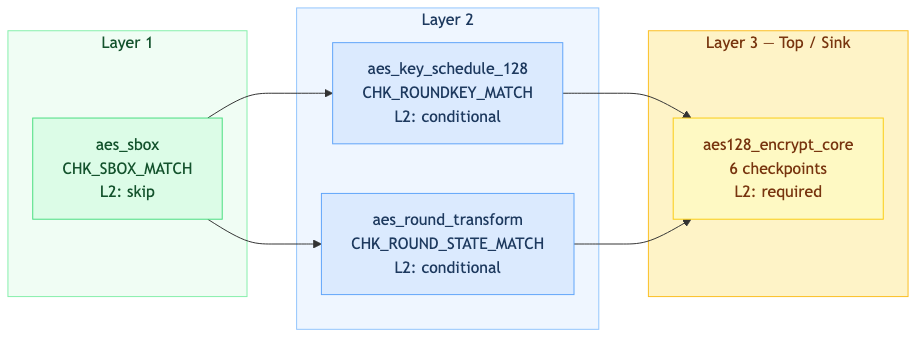
\includegraphics[keepaspectratio,alt={图 3-2: AES-128模块依赖DAG}]{../fpga_flow/diagrams/02_aes_node_dag.png}}
\caption{图 3-2: AES-128模块依赖DAG}
\end{figure}

4 个模块的角色与依赖关系如下：

\textbf{aes\_sbox（S-box 替换模块）}：实现 AES
标准中的字节替换操作，为纯组合逻辑，无上游依赖。该模块是 DAG
的叶节点（\texttt{integration\_role:\ leaf}），被
\texttt{aes\_key\_schedule\_128}、\texttt{aes\_round\_transform} 和
\texttt{aes128\_encrypt\_core}
三个模块依赖。由于其功能单一且无依赖，\texttt{l2\_policy} 设置为
\texttt{skip}（跳过鲁棒性测试）。

\textbf{aes\_key\_schedule\_128（密钥扩展模块）}：实现 AES-128
的密钥扩展算法，生成 11 组轮密钥（含初始密钥在内）。该模块依赖
\texttt{aes\_sbox}（用于 SubWord 操作），\texttt{l2\_policy} 为
\texttt{conditional}，\texttt{criticality} 为 \texttt{high}。

\textbf{aes\_round\_transform（轮变换模块）}：实现 AES 单轮的 4
步变换：SubBytes（字节替换）、ShiftRows（行移位）、MixColumns（列混合，基于
GF(2\^{}8) 有限域运算）和 AddRoundKey（轮密钥异或）。该模块依赖
\texttt{aes\_sbox}，\texttt{l2\_policy} 为
\texttt{conditional}，\texttt{criticality} 为 \texttt{high}。

\textbf{aes128\_encrypt\_core（顶层加密核心）}：实现 AES-128
加密的顶层有限状态机（FSM），集成上述全部子模块，实现 11 周期延迟（初始
AddRoundKey 1 周期 + 10 轮迭代各 1 周期）的 block-level handshake
接口。该模块是 DAG 的 sink
节点（\texttt{integration\_role:\ sink}），\texttt{l2\_policy} 为
\texttt{required}，\texttt{criticality} 为
\texttt{high}，是集成回归测试的顶层目标。

\subsubsection{3.2.2
模块端口规范}\label{ux6a21ux5757ux7aefux53e3ux89c4ux8303}

\textbf{表 3-2: 4 模块端口规范一览表}

{\def\LTcaptype{none} % do not increment counter
\begin{longtable}[]{@{}
  >{\raggedright\arraybackslash}p{(\linewidth - 8\tabcolsep) * \real{0.1875}}
  >{\raggedright\arraybackslash}p{(\linewidth - 8\tabcolsep) * \real{0.2500}}
  >{\raggedright\arraybackslash}p{(\linewidth - 8\tabcolsep) * \real{0.1875}}
  >{\raggedright\arraybackslash}p{(\linewidth - 8\tabcolsep) * \real{0.1875}}
  >{\raggedright\arraybackslash}p{(\linewidth - 8\tabcolsep) * \real{0.1875}}@{}}
\toprule\noalign{}
\begin{minipage}[b]{\linewidth}\raggedright
模块
\end{minipage} & \begin{minipage}[b]{\linewidth}\raggedright
信号名
\end{minipage} & \begin{minipage}[b]{\linewidth}\raggedright
方向
\end{minipage} & \begin{minipage}[b]{\linewidth}\raggedright
宽度
\end{minipage} & \begin{minipage}[b]{\linewidth}\raggedright
说明
\end{minipage} \\
\midrule\noalign{}
\endhead
\bottomrule\noalign{}
\endlastfoot
aes\_sbox & in\_byte & input & 8 & 待替换的输入字节 \\
aes\_sbox & out\_byte & output & 8 & 替换后的输出字节 \\
aes\_key\_schedule\_128 & key & input & 128 & AES-128 原始密钥 \\
aes\_key\_schedule\_128 & round\_keys & output & 1408 & 11
组轮密钥（11×128 bit） \\
aes\_round\_transform & state\_in & input & 128 & 轮变换输入状态 \\
aes\_round\_transform & round\_key & input & 128 & 本轮密钥 \\
aes\_round\_transform & is\_last\_round & input & 1 & 末轮标志（跳过
MixColumns） \\
aes\_round\_transform & state\_out & output & 128 & 轮变换输出状态 \\
aes128\_encrypt\_core & clk & input & 1 & 时钟信号 \\
aes128\_encrypt\_core & rst & input & 1 & 同步复位（高有效） \\
aes128\_encrypt\_core & start & input & 1 & 加密启动握手信号 \\
aes128\_encrypt\_core & plaintext & input & 128 & 明文输入 \\
aes128\_encrypt\_core & key & input & 128 & 加密密钥 \\
aes128\_encrypt\_core & ciphertext & output & 128 & 密文输出 \\
aes128\_encrypt\_core & done & output & 1 & 完成单周期脉冲 \\
aes128\_encrypt\_core & busy & output & 1 & 运算进行中标志 \\
\end{longtable}
}

上述接口规范在 \texttt{synthesis.py} 的 \texttt{\_aes\_blueprints()}
中以 \texttt{PortSpec} 字典形式定义，经
\texttt{ContractCompiler.compile\_module\_contract()} 转换为
\texttt{ModuleContract} 模型，并写入各模块工作区的
\texttt{module\_contract.json} 文件，成为 Agent
在生成和修复过程中不得更改的冻结接口约束。

\begin{center}\rule{0.5\linewidth}{0.5pt}\end{center}

\subsection{3.3 Agent 角色与 LLM
配置}\label{agent-ux89d2ux8272ux4e0e-llm-ux914dux7f6e}

\subsubsection{3.3.1 Agent
角色体系}\label{agent-ux89d2ux8272ux4f53ux7cfb}

本框架共定义 3 种 Agent 角色（由 \texttt{AgentRole} 枚举列出），对应 5
个 Agent 构建函数。\texttt{policy.py} 中的 \texttt{AgentRole}
枚举包含三个值：\texttt{WORKFLOW\_ORCHESTRATOR}（工作流编排器）、\texttt{MODULE\_WORKER\_SUBAGENT}（模块工作者子代理）和
\texttt{L2\_CAMPAIGN\_SUBAGENT}（L2
测试活动子代理）。\texttt{agents/specs.py} 中共提供 5
个构建函数：\texttt{build\_workflow\_orchestrator\_spec()} 和
\texttt{build\_finalizer\_orchestrator\_spec()} 均对应
\texttt{WORKFLOW\_ORCHESTRATOR}
角色（终态编排器复用编排器角色类型但使用不同的 LLM Profile
和工具集）；\texttt{build\_module\_worker\_spec()} 和
\texttt{build\_repair\_worker\_spec()} 均对应
\texttt{MODULE\_WORKER\_SUBAGENT}
角色（修复工作者复用模块工作者角色类型但不持有 \texttt{run\_executor}
工具）；\texttt{build\_l2\_campaign\_spec()} 对应
\texttt{L2\_CAMPAIGN\_SUBAGENT} 角色。每个构建函数返回的
\texttt{AgentSpawnSpec} 包含角色类型、LLM Profile、系统提示词、Skill
键集合、允许的编排器状态集合及可写路径约束。

具体来看，本框架设计了 5 个 Agent 构建函数：

\begin{itemize}
\tightlist
\item
  \texttt{build\_workflow\_orchestrator\_spec()}：构建执行编排器，使用
  \texttt{DEEPSEEK\_OFFICIAL\_FAST} profile，持有 \texttt{run\_executor}
  自定义工具，允许在除 \texttt{DONE} 之外的全部 9
  个状态下活动，不持有任何可写路径（编排器不直接写文件）。
\item
  \texttt{build\_finalizer\_orchestrator\_spec()}：构建终态汇总编排器，使用
  \texttt{DEEPSEEK\_OFFICIAL\_THINKING} profile，持有
  \texttt{FinishTool}，仅允许在
  \texttt{INTEGRATION\_READY}、\texttt{INTEGRATION\_REGRESSION}、\texttt{DONE}
  三个状态下活动，负责生成最终工作流报告后调用 \texttt{finish()}。
\item
  \texttt{build\_module\_worker\_spec(node)}：构建单模块工作者，使用
  \texttt{DEEPSEEK\_OFFICIAL\_FAST} profile，持有 \texttt{run\_executor}
  工具，可写路径严格限定为该节点的 RTL 文件和测试台文件，仅允许在
  \texttt{MODULE\_DESIGN}、\texttt{MODULE\_L0}、\texttt{MODULE\_L1}
  三个状态下活动。
\item
  \texttt{build\_repair\_worker\_spec()}：构建专用修复工作者，使用
  \texttt{DEEPSEEK\_OFFICIAL\_FAST} profile，不持有
  \texttt{run\_executor}（修复阶段不允许触发执行），遵循''编辑优先''协议。
\item
  \texttt{build\_l2\_campaign\_spec(node,\ ...)}：构建 L2
  测试活动代理，使用 \texttt{DEEPSEEK\_OFFICIAL\_FAST} profile，持有
  \texttt{run\_executor} 工具，仅允许在 \texttt{MODULE\_L2\_OPTIONAL}
  状态下活动，不允许 RTL 或测试台编辑。
\end{itemize}

\subsubsection{3.3.2 双 LLM Profile
策略}\label{ux53cc-llm-profile-ux7b56ux7565}

系统采用 \texttt{LLMProfileName} 枚举定义两种 DeepSeek API 调用配置：

\begin{itemize}
\tightlist
\item
  \texttt{DEEPSEEK\_OFFICIAL\_THINKING}（深度思考模式，\texttt{reasoning\_effort=\textquotesingle{}medium\textquotesingle{}}）：计算成本较高但推理能力强，用于需要跨模块推理的编排器（规格分析、架构设计、集成回归阶段）以及最终汇总编排器。
\item
  \texttt{DEEPSEEK\_OFFICIAL\_FAST}（快速执行模式，\texttt{reasoning\_effort=\textquotesingle{}none\textquotesingle{}}）：响应快速、成本低，用于局部任务执行的工作者（模块生成、验证、修复、L2
  测试）。
\end{itemize}

这一双 Profile
设计的核心逻辑是：跨模块决策（如判断模块间接口是否一致、决定是否升级）需要深度推理能力，而节点本地任务（如基于已有参考代码修复一个编译错误）不需要耗费推理资源，使用快速模式即可完成。通过在正确的任务上使用正确的
Profile，系统在保证决策质量的同时控制了 API 调用成本。

\textbf{表 3-3: Agent 角色-LLM Profile-工具矩阵}

{\def\LTcaptype{none} % do not increment counter
\begin{longtable}[]{@{}
  >{\raggedright\arraybackslash}p{(\linewidth - 6\tabcolsep) * \real{0.2444}}
  >{\raggedright\arraybackslash}p{(\linewidth - 6\tabcolsep) * \real{0.2889}}
  >{\raggedright\arraybackslash}p{(\linewidth - 6\tabcolsep) * \real{0.2000}}
  >{\raggedright\arraybackslash}p{(\linewidth - 6\tabcolsep) * \real{0.2667}}@{}}
\toprule\noalign{}
\begin{minipage}[b]{\linewidth}\raggedright
Agent 角色
\end{minipage} & \begin{minipage}[b]{\linewidth}\raggedright
LLM Profile
\end{minipage} & \begin{minipage}[b]{\linewidth}\raggedright
持有工具
\end{minipage} & \begin{minipage}[b]{\linewidth}\raggedright
典型活动状态
\end{minipage} \\
\midrule\noalign{}
\endhead
\bottomrule\noalign{}
\endlastfoot
执行编排器（Workflow Orchestrator） & FAST & run\_executor &
MODULE\_DESIGN / L0 / L1 \\
终态编排器（Finalizer Orchestrator） & THINKING & FinishTool &
INTEGRATION\_READY / DONE \\
模块工作者（Module Worker） & FAST & run\_executor & MODULE\_DESIGN / L0
/ L1 \\
修复工作者（Repair Worker） & FAST & 无 & MODULE\_DESIGN / L0 / L1 \\
L2 测试代理（L2 Campaign） & FAST & run\_executor &
MODULE\_L2\_OPTIONAL \\
\end{longtable}
}

\begin{center}\rule{0.5\linewidth}{0.5pt}\end{center}

\subsection{3.4 DAG
拓扑批调度与并行执行}\label{dag-ux62d3ux6251ux6279ux8c03ux5ea6ux4e0eux5e76ux884cux6267ux884c}

\subsubsection{3.4.1
拓扑分层算法}\label{ux62d3ux6251ux5206ux5c42ux7b97ux6cd5}

DAG 拓扑批调度是本框架处理多模块硬件设计的通用机制------对于任何 DAG
可分解的设计，\texttt{DAGBatchPlanner}
均可自动计算拓扑层级和并行批次。以下以 AES-128 的 4 节点 DAG
为具体示例说明其工作原理。

\texttt{synthesis.py} 中的 \texttt{DAGBatchPlanner} 类实现了基于 Kahn
算法变体的拓扑分层调度。\texttt{\_topological\_layers()}
方法计算每个节点的入度（依赖数量），将入度为 0
的节点放入初始就绪集合，按批次执行并在每次执行后将新满足依赖的节点加入下一批次。

对于 AES-128 的 4 节点 DAG，拓扑分层的结果为：

\begin{itemize}
\tightlist
\item
  \textbf{第一批次（Layer
  1）}：\texttt{{[}aes\_sbox{]}}------无依赖，单独执行。
\item
  \textbf{第二批次（Layer
  2）}：\texttt{{[}aes\_key\_schedule\_128,\ aes\_round\_transform,\ aes128\_encrypt\_core{]}}------在
  \texttt{aes\_sbox}
  完成后，三个模块的依赖均已满足，理论上可并行委派执行。
\end{itemize}

节点在同层内按优先级排序：首先按
\texttt{integration\_role}（\texttt{top} \textgreater{} \texttt{sink}
\textgreater{} \texttt{leaf} \textgreater{} \texttt{support}），其次按
\texttt{criticality}（\texttt{high} \textgreater{} \texttt{medium}
\textgreater{} \texttt{low}），最后按 \texttt{module\_id}
字母序。这一排序策略确保顶层/关键模块优先处理。

批次任务被封装为 \texttt{DelegateBatchPlan}，包含
\texttt{batch\_id}、\texttt{stage}（对应
\texttt{OrchestratorState}）、\texttt{max\_children}（最大子代理数，默认
5）和 \texttt{tasks} 列表。\texttt{max\_children}
限制了单批次并行子代理数量，防止对 LLM API 造成过大并发压力。

\begin{figure}
\centering
\pandocbounded{
\includegraphics[keepaspectratio,alt={图 3-3: 批次执行循环}]{../fpga_flow/diagrams/03_batch_execution_loop.png}}
\caption{图 3-3: 批次执行循环}
\end{figure}

\subsubsection{3.4.2
工作区生命周期状态机}\label{ux5de5ux4f5cux533aux751fux547dux5468ux671fux72b6ux6001ux673a}

每个节点的工作区存在独立的状态机，由 \texttt{NodeWorkspaceState}
枚举定义 7 个状态：

\begin{itemize}
\tightlist
\item
  \texttt{MISSING}：工作区尚未初始化
\item
  \texttt{DRAFT\_READY}：工作区已初始化、草稿文件已由 Memory 预填充
\item
  \texttt{VALIDATED}：L0 编译和 L1 仿真均通过，所有必需 Checkpoint 均为
  PASS
\item
  \texttt{PROMOTED}：已从草稿工作区晋升至规范 RTL/TB 路径
\item
  \texttt{REPAIRING}：验证失败，正在修复循环中（未超出预算）
\item
  \texttt{BLOCKED}：修复预算耗尽，需要人工介入或升级至思考型编排器
\item
  \texttt{FAILED}：发生不可恢复的错误
\end{itemize}

\texttt{NodePolicyEngine.decide\_next\_mode()} 根据当前
\texttt{NodeWorkspaceRecord} 状态和验证结果决定下一个
\texttt{SubagentWorkMode}（\texttt{GENERATE}、\texttt{VALIDATE}、\texttt{REPAIR}、\texttt{L2\_EXECUTE}
或 \texttt{INTEGRATION}）。这一决策逻辑完全在框架侧执行，LLM
无法直接影响工作区状态的推进。

\begin{center}\rule{0.5\linewidth}{0.5pt}\end{center}

\subsection{3.5
关键支撑机制概述}\label{ux5173ux952eux652fux6491ux673aux5236ux6982ux8ff0}

\subsubsection{3.5.1
结构化修复循环}\label{ux7ed3ux6784ux5316ux4feeux590dux5faaux73af}

当 L0 编译或 L1
仿真失败时，系统启动结构化修复循环。修复循环的完整流程为：

\begin{enumerate}
\def\labelenumi{\arabic{enumi}.}
\tightlist
\item
  \texttt{write\_repair\_request()} 生成 \texttt{RepairContract}
  并写入工作区，其中包含失败阶段（\texttt{failure\_phase}）、主要目标文件（\texttt{primary\_target\_file}）、文件片段（\texttt{primary\_file\_excerpt}）、错误摘要（\texttt{error\_excerpt}）、仿真日志摘要（\texttt{simulation\_log\_excerpt}）及第一步编辑指令（\texttt{first\_edit\_steps}）。
\item
  修复工作者 Agent 读取 \texttt{RepairContract}，按照
  \texttt{REPAIR\_PHASE\_ROUND\_1} 或
  \texttt{REPAIR\_PHASE\_ROUND\_2\_PLUS}
  阶段混入的约束执行精确编辑。第一轮修复的硬性要求是：\textbf{第一个工具调用必须是对
  \texttt{primary\_target\_file} 的文件编辑}，防止 Agent 偏离修复范围。
\item
  \texttt{verify\_repair\_edit()} 通过 SHA-256
  哈希比对验证文件确实发生了实质性变化，并检查
  \texttt{must\_add\_tokens}
  列表中的必要令牌是否已被添加。哈希验证失败意味着 Agent
  未实际修改文件，系统将拒绝该修复并记录失败。
\item
  \texttt{write\_edit\_receipt()} 写出
  \texttt{EditReceipt}，记录已编辑的文件列表和第一步编辑摘要。
\item
  重新触发 L0/L1 验证。
\end{enumerate}

\subsubsection{3.5.2 升级策略}\label{ux5347ux7ea7ux7b56ux7565}

\texttt{AgentExecutionPolicy.should\_escalate()}
是升级决策的唯一入口，当下列任一条件满足时返回 \texttt{True}：

\begin{itemize}
\tightlist
\item
  \texttt{repair\_attempts\ \textgreater{}=\ repair\_attempt\_threshold}（修复次数达到阈值，默认
  2 次）
\item
  \texttt{cross\_module\_issue=True}（问题跨越模块边界）
\item
  \texttt{state\_machine\_issue=True}（涉及状态机逻辑错误）
\item
  \texttt{interface\_issue=True}（涉及接口信号不兼容）
\end{itemize}

升级后，控制权从快速模式的工作者 Agent
返回至深度思考模式的编排器，携带完整的失败上下文（失败阶段、错误日志、已尝试的修复历史），由编排器决定后续策略（继续修复、放弃该节点或重新规划）。

\subsubsection{3.5.3 Pydantic
反幻觉机制}\label{pydantic-ux53cdux5e7bux89c9ux673aux5236}

所有合约模型均使用
\texttt{ConfigDict(extra=\textquotesingle{}forbid\textquotesingle{})}，这意味着任何
JSON 响应中出现的多余字段都会在反序列化时立即触发
\texttt{ValidationError}。结合 \texttt{@model\_validator}
中的范围约束（如 \texttt{SpecIR} 强制
\texttt{algorithm=\textquotesingle{}AES\textquotesingle{}}、\texttt{variant=\textquotesingle{}AES-128\textquotesingle{}}、\texttt{latency\_target\_cycles=11}），系统构建了一个机器可检查的约束体系，有效防止
LLM 幻觉污染核心数据结构。

\begin{center}\rule{0.5\linewidth}{0.5pt}\end{center}

本章从整体层面描述了框架的通用六层架构设计，并以 AES-128
验证案例展示了模块 DAG 分解、Agent 角色配置和 DAG
批调度的具体实例化。这一架构设计的核心优势在于：关注点分离（每层职责单一）、控制权内聚（框架而非
LLM
掌握进度判断）以及设计无关性（架构层面的通用性使其可适配不同的硬件设计目标）。后续各章将对状态机编排（第四章）、分层验证体系（第五章）和
LLM
约束引擎（第六章）三个核心创新点进行深入展开，每个创新点均先阐述通用设计原理，再以
AES-128 案例展示具体实例化。

\section{第四章
编排状态机与策略分层设计}\label{ux7b2cux56dbux7ae0-ux7f16ux6392ux72b6ux6001ux673aux4e0eux7b56ux7565ux5206ux5c42ux8bbeux8ba1}

编排状态机是本框架的核心控制机制，其设计面向通用的多模块硬件设计自动化流程。状态机定义的执行阶段（规格摄入→架构设计→规划→模块设计→分层验证→集成回归→终态）适用于任何
DAG 可分解的硬件设计任务。本章先阐述状态机的通用语义设计，再以 AES-128
验证案例展示各状态的具体实例化内容。

\subsection{4.1 10
状态编排状态机}\label{ux72b6ux6001ux7f16ux6392ux72b6ux6001ux673a}

\subsubsection{4.1.1
状态定义与语义}\label{ux72b6ux6001ux5b9aux4e49ux4e0eux8bedux4e49}

本框架的编排器状态机由 \texttt{policy.py} 中的
\texttt{OrchestratorState} 枚举完整定义，共包含 10 个状态。这 10
个状态不仅是系统执行阶段的语义标记，更是 \texttt{AgentExecutionPolicy}
映射的索引键------每个状态精确决定了当前阶段应使用哪种 LLM Profile
和哪种子代理委派策略。以下逐一说明各状态的语义与行为：

\textbf{（1）SPEC\_INTAKE（规格摄入）}

规格摄入状态是整个工作流的起点，负责将设计目标解析为框架可处理的结构化规格中间表示（\texttt{SpecIR}）。该状态适用于任何硬件设计目标------框架接收设计规格，验证其是否满足自动化前提条件，并生成后续阶段所需的元数据。

在 AES-128 验证案例中，\texttt{synthesize\_spec\_ir()} 从预设的 AES-128
目标中构建 \texttt{SpecIR}
数据模型，该模型包含系统目标、算法标识符、变体（\texttt{AES-128}）、操作类型（\texttt{encrypt}）、接口风格（\texttt{block\_handshake}）、微架构（\texttt{iterative\_10\_round}）、时序目标（延迟
11 周期）及冻结接口清单。由于 \texttt{SpecIR} 带有
\texttt{@model\_validator} 约束，若目标不符合 AES MVP
范围则立即报错。这一阶段的执行主体是框架合成层，而非 LLM，故分配
\texttt{DEEPSEEK\_OFFICIAL\_THINKING} profile（用于后续若需 LLM
辅助分析规格）且子代理策略为 \texttt{FORBIDDEN}。

\textbf{（2）ARCHITECTING（架构设计）}

在架构设计状态下，\texttt{synthesize\_plan\_dag()} 从
\texttt{\_aes\_blueprints()} 蓝图生成 \texttt{PlanDAG}，包含 4
个节点及其依赖关系，并通过内置的 DFS
无环验证。该状态同样以框架合成层为主体，LLM 参与程度最低，子代理策略为
\texttt{FORBIDDEN}。

\textbf{（3）PLANNING（规划）}

规划状态负责生成
\texttt{IntegrationRegressionManifest}（集成回归清单）并初始化
\texttt{FragilityMemory}（脆弱性历史记录），为后续批调度提供必要的元数据。子代理策略为
\texttt{FORBIDDEN}。

\textbf{（4）MODULE\_DESIGN（模块设计）}

模块设计状态是 LLM
首次深度介入的状态。在此状态下，\texttt{initialize\_node\_workspace()}
为每个节点创建工作区目录结构，生成
\texttt{module\_contract.json}、\texttt{testbench\_contract.json} 和
\texttt{module\_design\_brief.json} 三份合约文件，并通过
\texttt{MemoryStore.populate\_workspace()} 将来自 Skill
文件的验证通过参考代码写入草稿 RTL 和测试台文件。工作区状态从
\texttt{MISSING} 转变为 \texttt{DRAFT\_READY}。LLM Profile 切换为
\texttt{DEEPSEEK\_OFFICIAL\_FAST}，子代理策略为
\texttt{MODULE\_WORKER\_ALLOWED}------允许编排器将节点本地任务委派给模块工作者子代理。

\textbf{（5）MODULE\_L0（编译门控）}

L0 状态执行 Verilator 编译，仅验证 RTL
文件的语法合法性和端口声明正确性，不进行仿真。\texttt{L0Executor} 调用
\texttt{VerilatorMCPAdapter} 触发编译，解析编译器标准错误输出，生成
\texttt{compile.log} 和结构化的编译结果 JSON。L0
门控的设计意图是快速失败：语法错误通常在秒级内发现，无需等待仿真完成。LLM
Profile 为 \texttt{DEEPSEEK\_OFFICIAL\_FAST}，子代理策略为
\texttt{MODULE\_WORKER\_ALLOWED}。

\textbf{（6）MODULE\_L1（仿真与 Checkpoint 验证）}

L1 状态执行完整的编译-仿真流程，并通过 \texttt{CheckpointParser} 解析
\texttt{simulation.log} 中的
\texttt{CHECKPOINT\textbar{}\textless{}name\textgreater{}\textbar{}PASS\textbar{}\textless{}detail\textgreater{}}
协议行。\texttt{summarize\_required\_checkpoints()} 对比
\texttt{pass\_criteria} 中声明的必需 Checkpoint
名称与实际解析到的通过记录，生成结构化汇总。只有所有必需 Checkpoint 均为
PASS 时，节点工作区状态才转变为 \texttt{VALIDATED}。LLM Profile 为
\texttt{DEEPSEEK\_OFFICIAL\_FAST}，子代理策略为
\texttt{MODULE\_WORKER\_ALLOWED}。

\textbf{（7）MODULE\_L2\_OPTIONAL（条件性鲁棒测试）}

L2 鲁棒测试状态为可选状态，仅在节点的 \texttt{l2\_policy} 不为
\texttt{skip} 时触发。\texttt{L2AdaptivePlanner} 根据
\texttt{FragilityMemory} 中记录的历史失败信号自适应选择测试
profile（\texttt{rand\_small}、\texttt{rand\_large} 或
\texttt{edge\_cases}），以固定种子和可复现的向量集进行大量随机或边界向量测试。\texttt{L2CampaignExecutor}
在发现反例时写出 \texttt{counterexample.json}，并在测试结束时输出
\texttt{fragility\_summary.json}。LLM Profile 为
\texttt{DEEPSEEK\_OFFICIAL\_FAST}，子代理策略为
\texttt{L2\_CAMPAIGN\_ALLOWED}。

\textbf{（8）INTEGRATION\_READY（集成就绪）}

当所有 4 个节点均达到 \texttt{PROMOTED}
状态后，\texttt{IntegrationReadinessResolver} 检查依赖闭包的完整性，选取
\texttt{integration\_role} 为 \texttt{sink}
的节点（\texttt{aes128\_encrypt\_core}）作为集成顶层目标，触发状态机进入集成就绪状态。此状态无
LLM 执行任务，仅由框架侧计算，子代理策略为 \texttt{FORBIDDEN}，LLM
Profile 切换回
\texttt{DEEPSEEK\_OFFICIAL\_THINKING}（为后续集成回归的跨模块推理做准备）。

\textbf{（9）INTEGRATION\_REGRESSION（集成回归测试）}

集成回归状态执行三种 campaign：\texttt{baseline}（NIST
标准向量端到端加密正确性）、\texttt{back\_to\_back}（连续加密，验证 FSM
状态清理）和
\texttt{mid\_reset}（加密中途复位，验证恢复行为）。\texttt{IntegrationRegressionExecutor}
分别运行三种测试并汇总 Checkpoint 结果。LLM Profile 为
\texttt{DEEPSEEK\_OFFICIAL\_THINKING}，子代理策略为
\texttt{FORBIDDEN}（集成阶段由思考型编排器独占控制，不委派子代理）。

\textbf{（10）DONE（终态）}

DONE
是不可转移的终态。当集成回归测试通过后，\texttt{next\_state\_after\_success(INTEGRATION\_REGRESSION)}
返回 \texttt{DONE}，触发 \texttt{ExecutionSession} 启动最终汇总对话，由
\texttt{Finalizer\ Orchestrator}（使用
\texttt{DEEPSEEK\_OFFICIAL\_THINKING}）读取所有 artifact
生成终态报告，然后调用 \texttt{finish()}。

\begin{figure}
\centering
\pandocbounded{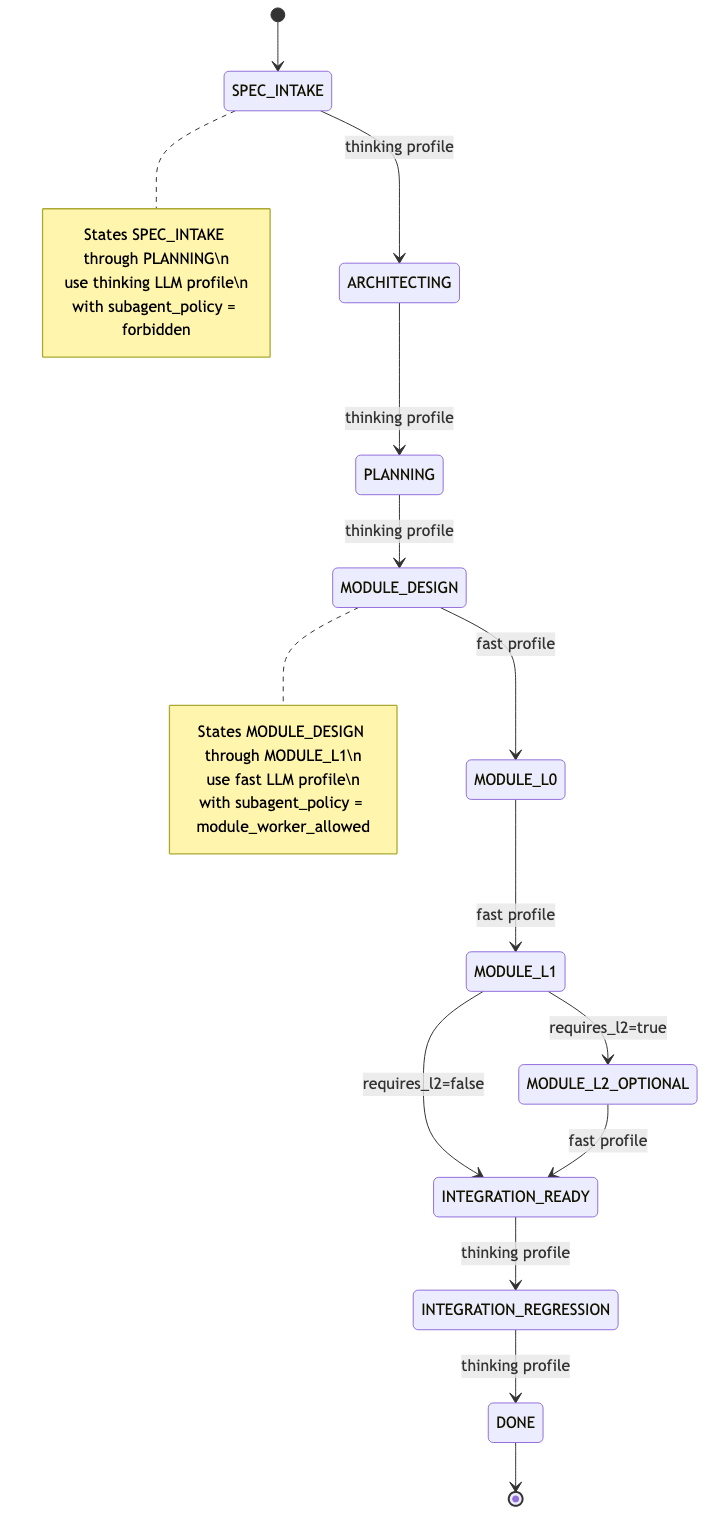
\includegraphics[keepaspectratio,alt={图 4-1: 编排器10状态转移图}]{../fpga_flow/diagrams/14_orchestrator_states.png}}
\caption{图 4-1: 编排器10状态转移图}
\end{figure}

\subsubsection{4.1.2
状态转移逻辑}\label{ux72b6ux6001ux8f6cux79fbux903bux8f91}

\texttt{AESWorkflowOrchestrator.next\_state\_after\_success()}
方法封装了所有成功路径的状态转移逻辑，其转移字典如下：

\begin{verbatim}
SPEC_INTAKE     → ARCHITECTING
ARCHITECTING    → PLANNING
PLANNING        → MODULE_DESIGN
MODULE_DESIGN   → MODULE_L0
MODULE_L0       → MODULE_L1
MODULE_L1       → MODULE_L2_OPTIONAL（当 requires_l2=True）
              → INTEGRATION_READY  （当 requires_l2=False）
MODULE_L2_OPTIONAL → INTEGRATION_READY
INTEGRATION_READY  → INTEGRATION_REGRESSION
INTEGRATION_REGRESSION → DONE
\end{verbatim}

\texttt{requires\_l2} 参数由节点的 \texttt{l2\_policy}
字段决定：\texttt{l2\_policy=\textquotesingle{}skip\textquotesingle{}}
时为
\texttt{False}，其他情况（\texttt{conditional}、\texttt{required}）为
\texttt{True}。\texttt{describe\_state\_progression()}
方法提供完整的状态链追踪，返回包含每个状态的 \texttt{StateTraceEntry}
列表，便于调试和日志记录。

\textbf{表 4-1: 每个状态的语义、执行者、输入/输出}

{\def\LTcaptype{none} % do not increment counter
\begin{longtable}[]{@{}
  >{\raggedright\arraybackslash}p{(\linewidth - 8\tabcolsep) * \real{0.1538}}
  >{\raggedright\arraybackslash}p{(\linewidth - 8\tabcolsep) * \real{0.1538}}
  >{\raggedright\arraybackslash}p{(\linewidth - 8\tabcolsep) * \real{0.2308}}
  >{\raggedright\arraybackslash}p{(\linewidth - 8\tabcolsep) * \real{0.2308}}
  >{\raggedright\arraybackslash}p{(\linewidth - 8\tabcolsep) * \real{0.2308}}@{}}
\toprule\noalign{}
\begin{minipage}[b]{\linewidth}\raggedright
状态
\end{minipage} & \begin{minipage}[b]{\linewidth}\raggedright
语义
\end{minipage} & \begin{minipage}[b]{\linewidth}\raggedright
执行主体
\end{minipage} & \begin{minipage}[b]{\linewidth}\raggedright
主要输入
\end{minipage} & \begin{minipage}[b]{\linewidth}\raggedright
主要输出
\end{minipage} \\
\midrule\noalign{}
\endhead
\bottomrule\noalign{}
\endlastfoot
SPEC\_INTAKE & 规格摄入与验证 & 框架合成层 & 系统目标字符串 & SpecIR \\
ARCHITECTING & DAG 结构生成 & 框架合成层 & SpecIR & PlanDAG \\
PLANNING & 集成清单生成 & 框架合成层 & SpecIR + PlanDAG &
IntegrationManifest \\
MODULE\_DESIGN & 工作区初始化与 Memory 预填充 & 框架 + Module Worker &
PlanDAGNode & 草稿 RTL/TB + 合约 JSON \\
MODULE\_L0 & 编译门控 & 框架 L0Executor & 草稿 RTL 文件 & compile.log +
编译结果 JSON \\
MODULE\_L1 & 仿真 + Checkpoint 验证 & 框架 L1Executor & 草稿 RTL + TB &
simulation.log + Checkpoint 汇总 \\
MODULE\_L2\_OPTIONAL & 鲁棒性随机测试 & 框架 L2CampaignExecutor + L2
Campaign Agent & 晋升 RTL + 向量集 & fragility\_summary.json +
counterexample.json \\
INTEGRATION\_READY & 依赖闭包验证 & 框架合成层 & 全部 PROMOTED 记录 &
集成顶层节点选择 \\
INTEGRATION\_REGRESSION & 三种集成 campaign & 框架
IntegrationRegressionExecutor & 集成清单 + 晋升 RTL & 三种 campaign
Checkpoint 结果 \\
DONE & 终态汇总 & Finalizer Orchestrator & 所有 artifact 路径 &
终态报告 \\
\end{longtable}
}

\begin{center}\rule{0.5\linewidth}{0.5pt}\end{center}

\subsection{4.2 AgentExecutionPolicy
策略分层}\label{agentexecutionpolicy-ux7b56ux7565ux5206ux5c42}

AgentExecutionPolicy 的设计是领域无关的------它将状态映射到 LLM Profile
和子代理策略，这一映射机制适用于任何硬件设计自动化场景。具体的映射内容基于通用的任务复杂度分析：跨模块决策需要深度推理，节点本地执行需要快速响应。

\subsubsection{4.2.1
策略模型设计}\label{ux7b56ux7565ux6a21ux578bux8bbeux8ba1}

\texttt{AgentExecutionPolicy} 是一个 Pydantic 模型（同样使用
\texttt{extra=\textquotesingle{}forbid\textquotesingle{}}），包含三个核心字段：

\begin{itemize}
\tightlist
\item
  \texttt{state\_profiles:\ dict{[}OrchestratorState,\ LLMProfileName{]}}：状态到
  LLM Profile 的映射
\item
  \texttt{state\_subagents:\ dict{[}OrchestratorState,\ SubagentPolicy{]}}：状态到子代理策略的映射
\item
  \texttt{repair\_attempt\_threshold:\ int}：修复升级阈值（默认 2，下限
  1）
\end{itemize}

\texttt{@model\_validator} 强制要求 \texttt{state\_profiles} 和
\texttt{state\_subagents} 必须覆盖全部 9 个活跃状态（\texttt{DONE}
状态不需要策略映射，因为它是终态）。这一完整性检查意味着系统永远不会出现''进入某个状态但找不到对应策略''的情况------若在系统初始化时发现缺失映射，将立即抛出
\texttt{ValueError} 阻止系统启动。

\subsubsection{4.2.2
完整策略映射表}\label{ux5b8cux6574ux7b56ux7565ux6620ux5c04ux8868}

\textbf{表 4-2: OrchestratorState → Policy 完整映射表}

{\def\LTcaptype{none} % do not increment counter
\begin{longtable}[]{@{}
  >{\raggedright\arraybackslash}p{(\linewidth - 6\tabcolsep) * \real{0.1622}}
  >{\raggedright\arraybackslash}p{(\linewidth - 6\tabcolsep) * \real{0.3243}}
  >{\raggedright\arraybackslash}p{(\linewidth - 6\tabcolsep) * \real{0.2703}}
  >{\raggedright\arraybackslash}p{(\linewidth - 6\tabcolsep) * \real{0.2432}}@{}}
\toprule\noalign{}
\begin{minipage}[b]{\linewidth}\raggedright
状态
\end{minipage} & \begin{minipage}[b]{\linewidth}\raggedright
LLM Profile
\end{minipage} & \begin{minipage}[b]{\linewidth}\raggedright
子代理策略
\end{minipage} & \begin{minipage}[b]{\linewidth}\raggedright
设计意图
\end{minipage} \\
\midrule\noalign{}
\endhead
\bottomrule\noalign{}
\endlastfoot
SPEC\_INTAKE & THINKING & FORBIDDEN & 规格验证需要精确推理，禁止委派 \\
ARCHITECTING & THINKING & FORBIDDEN & DAG 生成是框架操作，无 LLM 委派 \\
PLANNING & THINKING & FORBIDDEN & 集成清单生成，无子代理 \\
MODULE\_DESIGN & FAST & MODULE\_WORKER\_ALLOWED &
工作区初始化委派给节点工作者 \\
MODULE\_L0 & FAST & MODULE\_WORKER\_ALLOWED &
编译门控可委派给节点工作者 \\
MODULE\_L1 & FAST & MODULE\_WORKER\_ALLOWED &
仿真验证可委派给节点工作者 \\
MODULE\_L2\_OPTIONAL & FAST & L2\_CAMPAIGN\_ALLOWED & L2
测试专用子代理 \\
INTEGRATION\_READY & THINKING & FORBIDDEN & 集成就绪判断是框架操作 \\
INTEGRATION\_REGRESSION & THINKING & FORBIDDEN &
集成回归由思考型编排器独占 \\
\end{longtable}
}

\subsubsection{4.2.3 LLM Profile
分级的设计依据}\label{llm-profile-ux5206ux7ea7ux7684ux8bbeux8ba1ux4f9dux636e}

\texttt{LLMProfileName}
枚举定义了两个值：\texttt{DEEPSEEK\_OFFICIAL\_THINKING} 和
\texttt{DEEPSEEK\_OFFICIAL\_FAST}，分别对应深度思考模式和快速执行模式。

\textbf{使用思考模式（THINKING）的状态}：\texttt{SPEC\_INTAKE}、\texttt{ARCHITECTING}、\texttt{PLANNING}、\texttt{INTEGRATION\_READY}、\texttt{INTEGRATION\_REGRESSION}。这些状态涉及跨模块推理（如判断
4
个模块的接口是否一致）、工作流级别的决策（如决定是否触发升级）或需要精确分析集成测试失败原因。思考模式的
\texttt{reasoning\_effort=\textquotesingle{}medium\textquotesingle{}} 使
LLM
进行内部推理链（Chain-of-Thought），提升复杂推理的可靠性，但会增加延迟和
API 成本。

\textbf{使用快速模式（FAST）的状态}：\texttt{MODULE\_DESIGN}、\texttt{MODULE\_L0}、\texttt{MODULE\_L1}、\texttt{MODULE\_L2\_OPTIONAL}。这些状态的任务高度局部化------每个
Module Worker 只需要处理一个模块的代码，参考实现已通过 Memory
预填充，任务边界清晰。快速模式的
\texttt{reasoning\_effort=\textquotesingle{}none\textquotesingle{}}
跳过内部推理步骤，直接生成输出，响应时间显著降低。

\subsubsection{4.2.4 SubagentPolicy
三级控制}\label{subagentpolicy-ux4e09ux7ea7ux63a7ux5236}

\texttt{SubagentPolicy} 枚举定义了三个级别的子代理委派控制：

\textbf{FORBIDDEN（禁止委派）}：编排器不得在当前状态下启动子代理。适用于需要编排器独占控制的阶段：规格/架构/规划（这三个阶段由框架合成层执行，LLM
参与度低，不需要子代理）以及集成就绪/集成回归（这两个阶段需要跨模块推理，委派给子代理会导致上下文分散）。

\textbf{MODULE\_WORKER\_ALLOWED（允许模块工作者）}：编排器可以将节点本地任务委派给
Module Worker 子代理。Module Worker
的作用域严格限定：\texttt{build\_module\_worker\_spec()} 返回的
\texttt{AgentSpawnSpec} 中，\texttt{writable\_paths} 仅包含该节点的 RTL
文件和测试台文件，\texttt{allowed\_states} 仅包含
\texttt{MODULE\_DESIGN}/\texttt{MODULE\_L0}/\texttt{MODULE\_L1}
三个状态。这一双重约束（路径约束 + 状态约束）确保 Module Worker
无法越权修改其他模块的代码或执行集成级别的操作。

\textbf{L2\_CAMPAIGN\_ALLOWED（允许 L2 测试代理）}：编排器可以启动专用的
L2 测试活动子代理。L2 Campaign Agent 的
\texttt{build\_l2\_campaign\_spec()} 确保测试代理不持有 RTL/TB
可写路径，且持有的 \texttt{run\_executor} 工具在 L2
阶段不允许触发代码编辑操作。

\begin{figure}
\centering
\pandocbounded{
\includegraphics[keepaspectratio,alt={图 4-2: SDK Agent层级结构}]{../fpga_flow/diagrams/05_sdk_agent_hierarchy.png}}
\caption{图 4-2: SDK Agent层级结构}
\end{figure}

\begin{center}\rule{0.5\linewidth}{0.5pt}\end{center}

\subsection{4.3
升级策略设计}\label{ux5347ux7ea7ux7b56ux7565ux8bbeux8ba1}

\subsubsection{4.3.1
升级触发条件}\label{ux5347ux7ea7ux89e6ux53d1ux6761ux4ef6}

\texttt{AgentExecutionPolicy.should\_escalate()}
是系统中唯一的升级决策函数，其签名为：

\begin{Shaded}
\begin{Highlighting}[]
\KeywordTok{def}\NormalTok{ should\_escalate(}
    \VariableTok{self}\NormalTok{,}
\NormalTok{    repair\_attempts: }\BuiltInTok{int}\NormalTok{,}
    \OperatorTok{*}\NormalTok{,}
\NormalTok{    cross\_module\_issue: }\BuiltInTok{bool} \OperatorTok{=} \VariableTok{False}\NormalTok{,}
\NormalTok{    state\_machine\_issue: }\BuiltInTok{bool} \OperatorTok{=} \VariableTok{False}\NormalTok{,}
\NormalTok{    interface\_issue: }\BuiltInTok{bool} \OperatorTok{=} \VariableTok{False}\NormalTok{,}
\NormalTok{) }\OperatorTok{{-}\textgreater{}} \BuiltInTok{bool}\NormalTok{:}
    \ControlFlowTok{return}\NormalTok{ (}
\NormalTok{        repair\_attempts }\OperatorTok{\textgreater{}=} \VariableTok{self}\NormalTok{.repair\_attempt\_threshold}
        \KeywordTok{or}\NormalTok{ cross\_module\_issue}
        \KeywordTok{or}\NormalTok{ state\_machine\_issue}
        \KeywordTok{or}\NormalTok{ interface\_issue}
\NormalTok{    )}
\end{Highlighting}
\end{Shaded}

该函数的逻辑体现了两类不同性质的升级触发场景：

\textbf{数量触发}：当
\texttt{repair\_attempts\ \textgreater{}=\ repair\_attempt\_threshold}
时，说明 Module Worker
在有限次数内未能修复问题，继续让其尝试的边际收益递减。\texttt{repair\_attempt\_threshold}
默认为 2，即 Module Worker 最多允许两轮修复尝试。

\textbf{性质触发}：当
\texttt{cross\_module\_issue=True}（问题跨越模块边界，如接口信号宽度不匹配）、\texttt{state\_machine\_issue=True}（涉及
FSM 逻辑错误，如状态转移条件错误）或
\texttt{interface\_issue=True}（端口名称或方向不一致）时，无论已进行多少次修复，均立即升级。这三类问题的共同特征是：它们不能被节点本地的
Module Worker 独立解决，必须由具有全局视野的思考型编排器介入。

\subsubsection{4.3.2
修复预算管理}\label{ux4feeux590dux9884ux7b97ux7ba1ux7406}

\texttt{generation.py} 中的 \texttt{repair\_budget\_for\_node()}
函数根据节点的 \texttt{integration\_role} 字段分配差异化的修复预算：

\begin{Shaded}
\begin{Highlighting}[]
\KeywordTok{def}\NormalTok{ repair\_budget\_for\_node(node: PlanDAGNode) }\OperatorTok{{-}\textgreater{}} \BuiltInTok{int}\NormalTok{:}
    \ControlFlowTok{if}\NormalTok{ node.integration\_role }\KeywordTok{in}\NormalTok{ (}\StringTok{\textquotesingle{}top\textquotesingle{}}\NormalTok{, }\StringTok{\textquotesingle{}sink\textquotesingle{}}\NormalTok{):}
        \ControlFlowTok{return}\NormalTok{ TOP\_MODULE\_REPAIR\_BUDGET  }\CommentTok{\# = 3}
    \ControlFlowTok{return}\NormalTok{ DEFAULT\_REPAIR\_BUDGET  }\CommentTok{\# = 2}
\end{Highlighting}
\end{Shaded}

顶层/sink
节点（\texttt{aes128\_encrypt\_core}，\texttt{integration\_role=\textquotesingle{}sink\textquotesingle{}}）获得
3 次修复机会，其他节点（叶节点和支撑节点）获得 2
次机会。这一差异化预算设计的依据是：顶层加密核心是整个系统最复杂的模块，其
FSM 逻辑（\texttt{IDLE}→\texttt{ROUND}→\texttt{DONE}
三状态）涉及多个子模块的集成，修复时更容易需要多轮迭代。相比之下，\texttt{aes\_sbox}
等叶节点逻辑简单，若 2 次修复后仍失败，说明问题已超出 Module Worker
的能力范围，升级至编排器处理更为合适。

这一有限预算机制与基于AutoGen的线性pipeline方案中 Debug Agent
的无限重试策略形成鲜明对比：无限重试在理论上提供了更多自我修复机会，但在实践中可能导致系统陷入无效循环（例如
Agent 每次修复都破坏了其他已通过的
Checkpoint），且没有收敛保证。有限预算确保了系统的终止性。

\subsubsection{4.3.3
升级后的行为}\label{ux5347ux7ea7ux540eux7684ux884cux4e3a}

升级发生后，框架将失败模块的完整上下文（\texttt{RepairContract}、验证日志路径、已尝试的修复历史）附加到编排器会话的下一条消息中。思考型编排器在接收到升级信息后，可以采取以下几种策略之一：

\begin{itemize}
\tightlist
\item
  重新分析错误，生成新的 \texttt{RepairContract} 并重置修复计数
\item
  判断该模块为不可修复（\texttt{BLOCKED}
  状态），记录失败并继续处理其他节点
\item
  判断问题为跨模块接口不兼容，触发对相关模块的联合修复
\end{itemize}

\begin{figure}
\centering
\pandocbounded{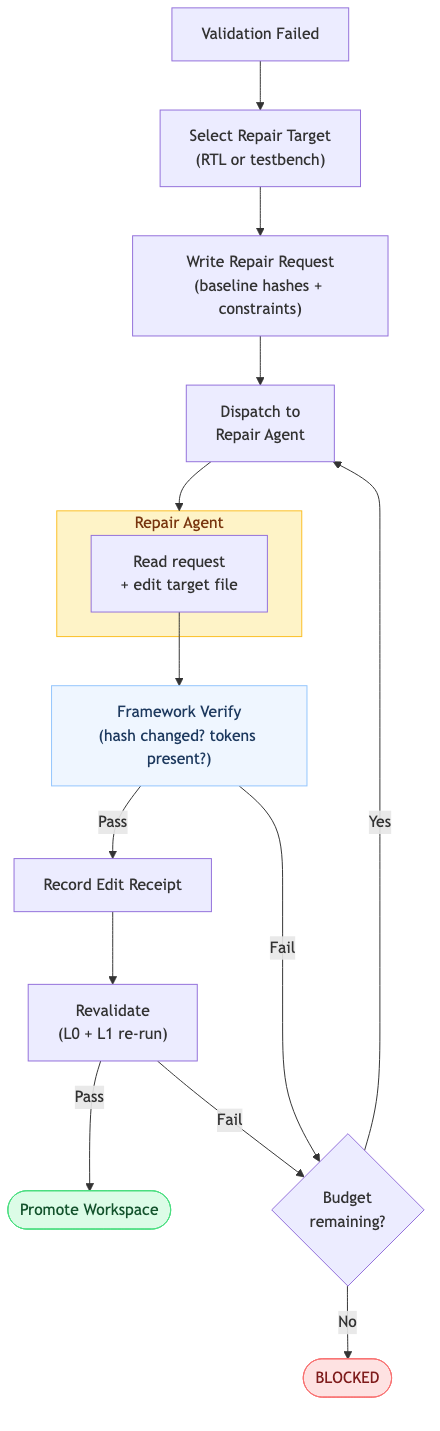
\includegraphics[keepaspectratio,alt={图 4-3: 修复循环流程}]{../fpga_flow/diagrams/06_repair_cycle.png}}
\caption{图 4-3: 修复循环流程}
\end{figure}

\begin{center}\rule{0.5\linewidth}{0.5pt}\end{center}

\subsection{4.4 框架控制 vs Agent
控制}\label{ux6846ux67b6ux63a7ux5236-vs-agent-ux63a7ux5236}

\subsubsection{4.4.1
核心设计决策}\label{ux6838ux5fc3ux8bbeux8ba1ux51b3ux7b56}

框架控制与 Agent
控制的对比分析适用于所有多智能体硬件设计自动化场景，不限于 AES-128
案例。LLM
在控制流中的典型失败模式（提前宣告成功、无限修复循环、范围漂移）是所有
LLM 驱动的工程自动化系统面临的共性挑战。

``为什么不让 LLM
决定何时推进工作流状态？''这一问题是本框架最核心的设计决策点。理解这一决策需要首先分析
LLM 在控制流场景中的典型失败模式。

\textbf{失败模式一：提前宣告成功（幻觉）}。LLM
在生成响应时可能基于局部信息做出乐观判断------例如，仿真输出中出现了''PASS''字样（但这是某个非必需
Checkpoint 的 PASS），LLM
便宣告该模块已通过验证，触发晋升操作。实际上，\texttt{CHK\_CIPHERTEXT\_MATCH}
这一关键 Checkpoint 从未出现在日志中。在 Prompt-controlled
方案中，这类幻觉式提前完成极难通过提示词工程杜绝；在本框架中，由于
Checkpoint 汇总由 \texttt{summarize\_required\_checkpoints()}
机器执行，LLM 的任何''宣告''都不会影响工作区状态的实际转变。

\textbf{失败模式二：无限修复循环}。LLM
在修复代码时可能反复修改同一段逻辑，每次修改都基于对错误的不同解读，但始终无法触达根本原因。没有外部预算限制的情况下，这种行为可以持续很长时间，消耗大量
API 调用和等待时间。本框架通过 \texttt{repair\_attempt\_threshold}
硬性终止修复循环，确保系统不会无限等待 LLM 的自我修复收敛。

\textbf{失败模式三：范围漂移（Scope Drift）}。LLM
在修复某个模块时可能''顺手''修改了其他模块的接口定义，以期解决接口不一致问题。这种越界修改在当时可能让测试通过，但破坏了系统的其他部分。\texttt{WORKER\_LOCAL\_SCOPE}
阶段混入约束从提示词层面限制 Agent
的行为范围，但更根本的保护来自框架层面的可写路径约束------\texttt{build\_module\_worker\_spec(node)}
生成的 \texttt{AgentSpawnSpec} 中，\texttt{writable\_paths}
仅包含该节点的文件，OpenHands SDK 在底层强制执行此约束。

\subsubsection{4.4.2 FRAMEWORK\_OWNS\_PROGRESS\_CONTRACT
的设计意图}\label{framework_owns_progress_contract-ux7684ux8bbeux8ba1ux610fux56fe}

\texttt{prompt\_contracts.py} 中的
\texttt{FRAMEWORK\_OWNS\_PROGRESS\_CONTRACT} 是一个
\texttt{BaseContract}，包含以下约束行：

\begin{verbatim}
The framework, not you, owns batch progression and workflow completion.
\end{verbatim}

这条约束被注入所有 Agent 角色的系统提示词，配合
\texttt{ORCHESTRATOR\_NO\_FINISH}
阶段混入（\texttt{Do\ not\ call\ finish\ in\ the\ execution\ conversation.}）和
\texttt{ORCHESTRATOR\_ONLY\_CURRENT\_BATCH}
阶段混入（\texttt{Execute\ only\ the\ current\ batch\ handed\ to\ this\ conversation.\ Do\ not\ infer\ future\ batches,\ merge\ batches,\ or\ summarize\ the\ whole\ workflow\ as\ complete.}），构建了三重语义锁定：

\begin{enumerate}
\def\labelenumi{\arabic{enumi}.}
\tightlist
\item
  \textbf{控制权归属声明}：明确告知 Agent 它不拥有工作流推进的控制权
\item
  \textbf{行动禁止规则}：禁止执行编排器调用 \texttt{finish()}
\item
  \textbf{批次边界约束}：禁止 Agent 基于推断跨越批次边界
\end{enumerate}

三重约束共同作用，确保即使在 LLM
产生错误乐观判断时，其输出也不会导致工作流状态的错误推进。

\subsubsection{4.4.3 Batch Gate
回调模式}\label{batch-gate-ux56deux8c03ux6a21ux5f0f}

\texttt{ConversationRunner.run\_current\_batch\_until\_gate()} 实现了
Batch Gate（批次门控）模式，这是框架控制架构的运行时实现：

\begin{Shaded}
\begin{Highlighting}[]
\KeywordTok{def}\NormalTok{ run\_current\_batch\_until\_gate(}
    \VariableTok{self}\NormalTok{,}
\NormalTok{    conversation,}
\NormalTok{    message: }\BuiltInTok{str}\NormalTok{,}
    \OperatorTok{*}\NormalTok{,}
\NormalTok{    batch\_gate: Callable[[], }\BuiltInTok{bool}\NormalTok{],}
\NormalTok{    timeout\_s: }\BuiltInTok{float} \OperatorTok{=} \FloatTok{180.0}\NormalTok{,}
\NormalTok{    poll\_interval\_s: }\BuiltInTok{float} \OperatorTok{=} \FloatTok{0.2}\NormalTok{,}
\NormalTok{) }\OperatorTok{{-}\textgreater{}}\NormalTok{ BatchRunSummary:}
\end{Highlighting}
\end{Shaded}

该方法的工作机制如下： 1. 向 Agent
会话发送当前批次任务消息，在独立线程中启动 Agent 对话循环 2. 主线程以
0.2 秒间隔轮询 \texttt{batch\_gate()} 回调（该回调检查文件系统中的
artifact 是否满足批次完成条件） 3. 当 \texttt{batch\_gate()} 返回
\texttt{True} 时，立即调用 \texttt{conversation.pause()} 暂停 Agent
会话，不等待 Agent 自行结束 4. 若超过 \texttt{timeout\_s}
秒后门控仍未满足，强制暂停会话并记录超时状态

这一模式的关键特征是：\textbf{文件系统是 Agent
与框架之间的唯一通信通道}。Agent 通过写文件（生成
RTL、写出编辑收据、输出验证报告）向框架传递工作进度；框架通过读文件（检查
\texttt{NodeWorkspaceRecord} 状态、解析 \texttt{EditReceipt}、校验
Checkpoint 汇总）判断批次是否完成。这种设计有两个重要优点：一是 Agent
的任何言辞性声明（``我已完成此模块''）不产生任何框架层面的效果；二是文件系统的持久性使得即使
Agent 会话意外终止，框架也能从 artifact 文件中恢复工作状态。

\begin{figure}
\centering
\pandocbounded{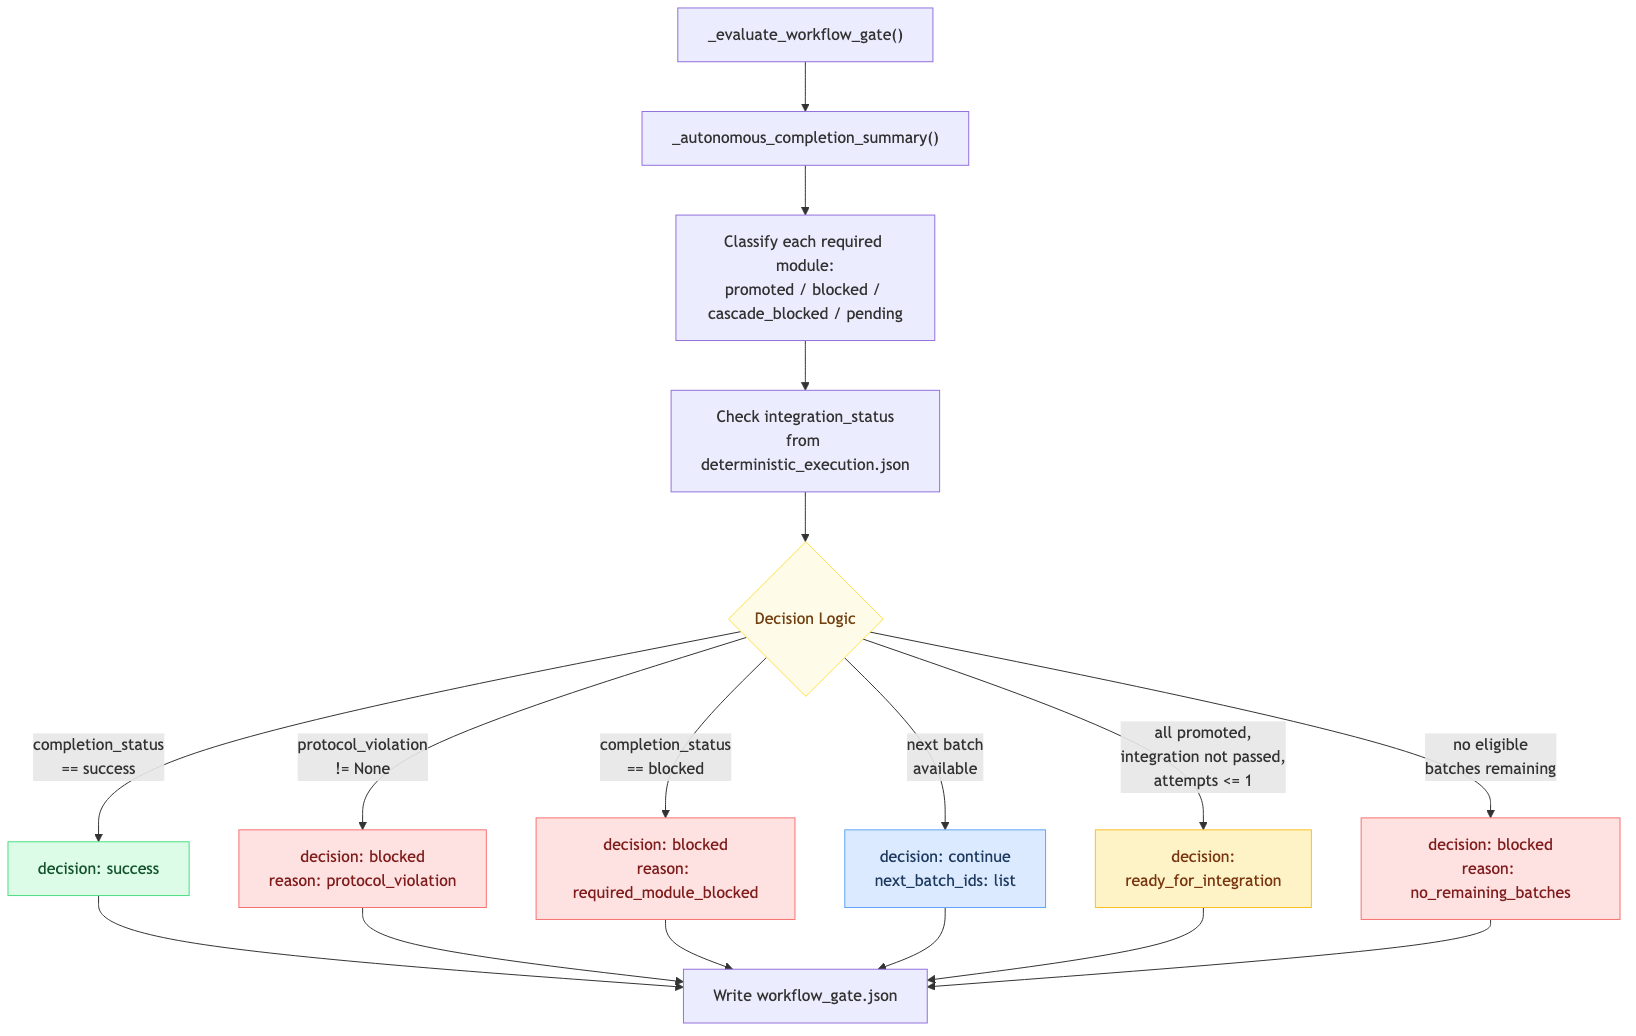
\includegraphics[keepaspectratio,alt={图 4-4: 工作流门控机制}]{../fpga_flow/diagrams/09_workflow_gate.png}}
\caption{图 4-4: 工作流门控机制}
\end{figure}

\subsubsection{4.4.4 与 AutoGen
方案的对比分析}\label{ux4e0e-autogen-ux65b9ux6848ux7684ux5bf9ux6bd4ux5206ux6790}

AutoGen 方案采用 AutoGen 的 \texttt{human\_input\_mode="NEVER"} 配置，使
Agent 链在无人工干预的情况下自主运行至完成。这一配置的含义是：AutoGen
的每个 Agent
在完成自己的任务后，自主决定是否结束对话或将控制权传递给下一个
Agent。控制流本质上由 LLM 的输出决定------当 Agent
输出''TERMINATE''关键词时，对话结束。

这种方式的主要风险在于：控制流的可靠性完全依赖 LLM
在正确时机输出正确关键词。若 LLM
错误地在验证尚未完成时输出''TERMINATE''，整个工作流便提前结束；若 LLM
陷入循环而不输出终止信号，工作流便永不结束。缺乏外部检查点（Checkpoint）意味着工作流的中间状态完全不透明。

本框架通过状态机 + Batch Gate +
\texttt{FRAMEWORK\_OWNS\_PROGRESS\_CONTRACT}
三层机制，将控制流的可靠性从''依赖 LLM
的正确输出''提升到''依赖框架代码的正确执行''。这一转变使系统的可靠性具备了数学可验证性：只要框架代码（Python
+ Pydantic）正确，批次推进决策就不会受到 LLM 幻觉的干扰。

\begin{center}\rule{0.5\linewidth}{0.5pt}\end{center}

\subsection{4.5 小结}\label{ux5c0fux7ed3}

本章深入分析了系统的 10 状态编排状态机与 \texttt{AgentExecutionPolicy}
策略分层机制。核心设计理念可归纳为三点：

\textbf{第一，状态语义精确化}。10 个状态不仅是阶段标记，更是 LLM Profile
选择和子代理委派策略的索引键，每个状态的语义与其对应的策略绑定。\texttt{AgentExecutionPolicy}
的完整性验证确保策略映射在系统初始化时即经过检查，而非在运行时动态推断。

\textbf{第二，策略分层精准化}。THINKING/FAST 双 Profile
的分配规则是：跨模块推理用 THINKING，节点本地执行用
FAST。FORBIDDEN/MODULE\_WORKER\_ALLOWED/L2\_CAMPAIGN\_ALLOWED
三级子代理策略的分配规则是：需要全局视野的阶段禁止委派，需要并行执行的节点本地任务允许委派给专用子代理。

\textbf{第三，控制权内聚于框架}。通过
\texttt{FRAMEWORK\_OWNS\_PROGRESS\_CONTRACT}、\texttt{ORCHESTRATOR\_NO\_FINISH}、\texttt{batch\_gate}
回调和有限修复预算四层机制，系统确保了工作流推进决策始终由可验证的框架代码而非不可靠的
LLM 输出驱动。这是本框架区别于传统 Prompt-controlled
多智能体方案的根本性架构差异，也是系统在面对 LLM
幻觉和不可靠性时保持工作流正确性的核心保障。

本章阐述的编排状态机与策略分层机制在架构层面是通用的：状态语义、策略映射和控制权分配原则均不依赖于特定的硬件设计对象。AES-128
验证案例中的具体实例化内容是案例相关的，但框架的状态机骨架和策略分层逻辑可直接复用于其他
DAG 可分解的多模块设计。

\section{第五章
四层验证体系与Checkpoint协议}\label{ux7b2cux4e94ux7ae0-ux56dbux5c42ux9a8cux8bc1ux4f53ux7cfbux4e0echeckpointux534fux8bae}

\subsection{5.1
分层验证架构}\label{ux5206ux5c42ux9a8cux8bc1ux67b6ux6784}

\subsubsection{5.1.1 设计动机}\label{ux8bbeux8ba1ux52a8ux673a}

在任何多智能体 FPGA
设计自动化框架中，验证是保证生成代码正确性的核心环节。本框架提出的四层分级验证体系是一种通用的硬件验证方法论，适用于任何具备
Verilator 可编译 RTL 和自检 C++ Testbench
的多模块设计。传统单层验证方案（仿真通过/失败）存在以下问题：其一，语法错误只有在仿真阶段才被发现，浪费了编译资源；其二，仿真通过并不能保证边界行为的正确性；其三，子模块的独立验证通过并不意味着顶层集成的正确性。

本文提出四层分级验证体系，遵循''快速失败（fail
fast）``原则，通过逐步深入的验证策略将问题发现尽可能提前，并将验证结果与框架控制流深度集成。

\begin{figure}
\centering
\pandocbounded{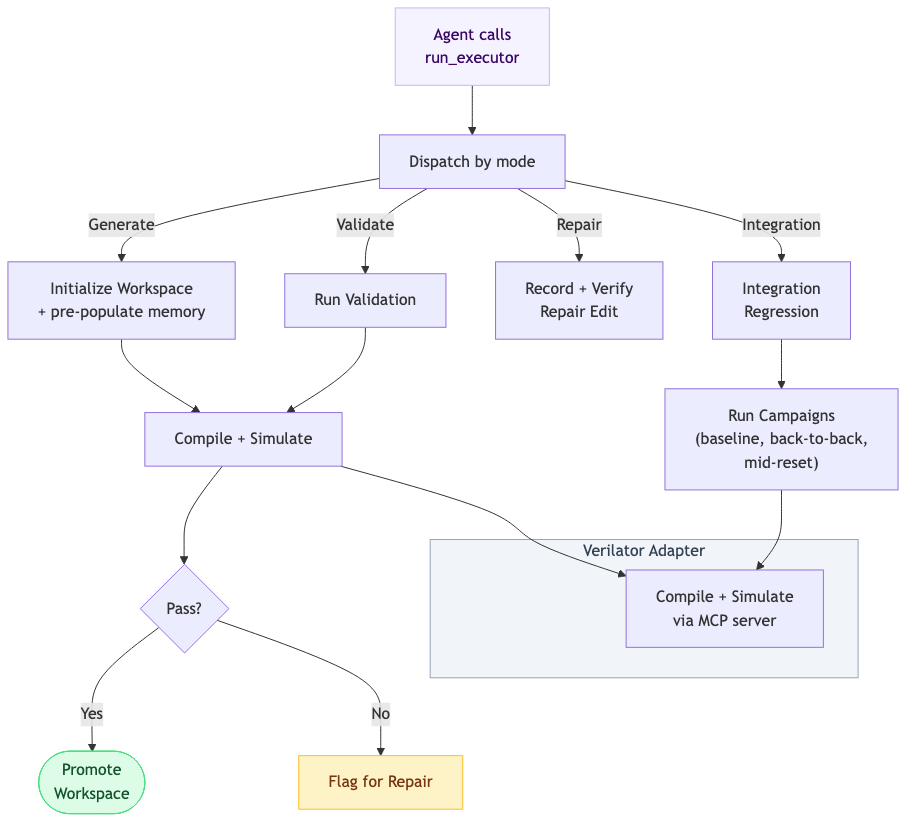
\includegraphics[keepaspectratio,alt={图5-1: 执行器调度流程}]{../fpga_flow/diagrams/08_executor_dispatch.png}}
\caption{图5-1: 执行器调度流程}
\end{figure}

四层验证体系的核心设计理念是：\textbf{时间成本与问题发现深度呈正比递增}。L0编译门控仅需秒级时间即可捕获语法级错误；L1仿真验证需要数十秒，但可验证功能正确性；L2鲁棒性测试需要分钟级时间，但能发现边界条件下的脆弱性；集成回归测试最为耗时，但能捕获模块间接口和时序问题。这一设计使系统能够在不同阶段以匹配的代价发现相应类型的问题。

\subsubsection{5.1.2
四层架构总览}\label{ux56dbux5c42ux67b6ux6784ux603bux89c8}

四层验证架构的设计不依赖于特定的硬件设计------L0 编译门控对任何 Verilog
RTL 有效，L1 Checkpoint 验证对任何实现了 Checkpoint 协议的 Testbench
有效，L2 鲁棒性测试对任何可参数化的 Testbench 有效，集成回归对任何 DAG
结构的多模块设计有效。以下以 AES-128 验证案例说明各层的具体运作。

各层验证的职责、输入输出与判定标准如下：

{[}表5-1: 各层级验证目标、输入、输出、判定标准、典型耗时{]}

\textbf{L0编译门控（L0Executor）}：接收RTL Verilog源文件和C++
Testbench，调用Verilator编译器，输出编译日志。判定标准为编译返回码为零且无错误输出。L0是最轻量的门控，能捕获未声明信号、端口宽度不匹配、语法错误、非法Verilog结构等问题。

\textbf{L1仿真验证（L1Executor）}：在L0编译成功的前提下执行仿真，通过解析\texttt{simulation.log}中的Checkpoint协议行判定功能正确性。L1采用已知向量（KAT，Known-Answer
Test），要求所有必需Checkpoint均出现且状态为PASS。

\textbf{L2鲁棒性测试（L2CampaignExecutor）}：对已通过L1的模块施加随机向量或边界向量的压力测试，验证在非KAT条件下的行为一致性。L2的判定不仅包含Checkpoint通过率，还会输出\texttt{counterexample.json}和\texttt{fragility\_summary.json}，供\texttt{L2AdaptivePlanner}用于后续Profile选择决策。

\textbf{集成回归测试（IntegrationRegressionExecutor）}：在所有模块全部PROMOTED后触发，以\texttt{IntegrationRegressionManifest}为规格驱动，对顶层模块\texttt{aes128\_encrypt\_core}执行三种Campaign（baseline、back\_to\_back、mid\_reset），验证完整系统在不同使用场景下的正确性。

\subsubsection{5.1.3
分层验证与框架控制流的集成}\label{ux5206ux5c42ux9a8cux8bc1ux4e0eux6846ux67b6ux63a7ux5236ux6d41ux7684ux96c6ux6210}

四层验证不是孤立存在的，而是与编排状态机深度集成。编排状态\texttt{MODULE\_L0}对应L0执行，\texttt{MODULE\_L1}对应L1执行，\texttt{MODULE\_L2\_OPTIONAL}对应L2鲁棒性测试，\texttt{INTEGRATION\_REGRESSION}对应集成回归测试。每层验证的判定结果直接影响工作区状态机的转移：L0失败则工作区保持REPAIRING状态，L1
Checkpoint全部通过则状态跃迁至VALIDATED，PROMOTED后触发集成回归。这一设计确保了验证结果的机器可判定性，消除了对LLM主观判断的依赖。

\begin{center}\rule{0.5\linewidth}{0.5pt}\end{center}

\subsection{5.2
Checkpoint协议设计}\label{checkpointux534fux8baeux8bbeux8ba1}

\subsubsection{5.2.1
协议格式规范}\label{ux534fux8baeux683cux5f0fux89c4ux8303}

Checkpoint 协议的格式设计是完全通用的------任何硬件设计的 Testbench
均可通过调用 \texttt{emit\_checkpoint()} 发射自定义的 Checkpoint
标记，框架的 \texttt{CheckpointParser}
无需修改即可解析。协议的通用性使得框架支持新设计时无需更改验证基础设施，只需定义新的
Checkpoint 名称集合。

Checkpoint协议是本框架验证体系的核心通信机制，定义了Testbench与框架之间的结构化结果汇报接口。协议格式为：

\begin{verbatim}
CHECKPOINT|<name>|PASS|<detail>
\end{verbatim}

其中： - \texttt{CHECKPOINT} 为固定前缀，作为日志行过滤的识别标记 -
\texttt{\textless{}name\textgreater{}}
为Checkpoint名称，与\texttt{pass\_criteria.l1.coverage\_checkpoints}中定义的名称精确对应
- \texttt{PASS} 为当前唯一合法的状态值，表示该检查点已验证通过 -
\texttt{\textless{}detail\textgreater{}}
为人类可读的补充说明，不参与机器判定逻辑

该协议通过\texttt{aes\_tb\_common.hpp}中的\texttt{emit\_checkpoint()}函数在C++
Testbench端发射：

\begin{Shaded}
\begin{Highlighting}[]
\KeywordTok{inline} \DataTypeTok{void}\NormalTok{ emit\_checkpoint}\OperatorTok{(}
    \AttributeTok{const} \BuiltInTok{std::}\NormalTok{string}\OperatorTok{\&}\NormalTok{ checkpoint}\OperatorTok{,}
    \AttributeTok{const} \BuiltInTok{std::}\NormalTok{string}\OperatorTok{\&}\NormalTok{ detail}
\OperatorTok{)} \OperatorTok{\{}
    \BuiltInTok{std::}\NormalTok{cout }\OperatorTok{\textless{}\textless{}} \StringTok{"CHECKPOINT|"} \OperatorTok{\textless{}\textless{}}\NormalTok{ checkpoint }\OperatorTok{\textless{}\textless{}} \StringTok{"|PASS|"} \OperatorTok{\textless{}\textless{}}\NormalTok{ detail }\OperatorTok{\textless{}\textless{}} \BuiltInTok{std::}\NormalTok{endl}\OperatorTok{;}
\OperatorTok{\}}
\end{Highlighting}
\end{Shaded}

（\texttt{fpga\_flow/tb/aes\_tb\_common.hpp:603-608}）

这一设计实现了Testbench端的极简接入：Testbench开发者只需在正确性验证通过后调用\texttt{emit\_checkpoint("CHK\_XXX",\ "描述")}一行代码，无需了解协议解析细节。

\subsubsection{5.2.2
设计决策分析}\label{ux8bbeux8ba1ux51b3ux7b56ux5206ux6790}

选择简单文本协议而非结构化输出（如JSON）的决策基于以下考量：

\textbf{对日志噪声的鲁棒性}：Verilator仿真过程中会产生大量警告、调试输出和波形信息。文本协议通过逐行扫描和前缀匹配实现解析，不受日志噪声干扰；而JSON格式需要完整解析仿真输出流，对格式错误极为敏感。

\textbf{Testbench端实现简单}：\texttt{emit\_checkpoint()}是单行调用，Testbench开发者和LLM
Agent均能可靠地生成该调用，不会因JSON转义、嵌套结构等问题引入格式错误。

\textbf{框架端解析简单}：\texttt{CheckpointParser}（\texttt{fpga\_flow/executors.py:71-90}）的实现仅需30行代码，通过\texttt{CHECKPOINT\_PREFIX\ =\ \textquotesingle{}CHECKPOINT\textbar{}\textquotesingle{}}前缀过滤和\texttt{split(\textquotesingle{}\textbar{}\textquotesingle{},\ 3)}分割即可完成解析，维护成本极低。

与AutoGen方案的对比：该方案使用Vivado
xsim仿真，验证结果依赖波形图（.vcd）的人工判读，无法实现机器自动判定。本文的Checkpoint协议使验证结果完全机器可判定，且与文件系统通信机制（Batch
Gate回调）无缝集成。

\subsubsection{5.2.3
CheckpointParser解析逻辑}\label{checkpointparserux89e3ux6790ux903bux8f91}

框架端的\texttt{CheckpointParser}类（\texttt{fpga\_flow/executors.py:71-90}）负责从\texttt{simulation.log}文件中提取Checkpoint信息，构建\texttt{name→status\textbar{}detail}字典：

\begin{Shaded}
\begin{Highlighting}[]
\KeywordTok{class}\NormalTok{ CheckpointParser:}
    \KeywordTok{def}\NormalTok{ parse\_text(}\VariableTok{self}\NormalTok{, text: }\BuiltInTok{str}\NormalTok{) }\OperatorTok{{-}\textgreater{}} \BuiltInTok{dict}\NormalTok{[}\BuiltInTok{str}\NormalTok{, }\BuiltInTok{str}\NormalTok{]:}
\NormalTok{        summary: }\BuiltInTok{dict}\NormalTok{[}\BuiltInTok{str}\NormalTok{, }\BuiltInTok{str}\NormalTok{] }\OperatorTok{=}\NormalTok{ \{\}}
        \ControlFlowTok{for}\NormalTok{ raw\_line }\KeywordTok{in}\NormalTok{ text.splitlines():}
\NormalTok{            line }\OperatorTok{=}\NormalTok{ raw\_line.strip()}
            \ControlFlowTok{if} \KeywordTok{not}\NormalTok{ line.startswith(CHECKPOINT\_PREFIX):}
                \ControlFlowTok{continue}
\NormalTok{            parts }\OperatorTok{=}\NormalTok{ line.split(}\StringTok{\textquotesingle{}|\textquotesingle{}}\NormalTok{, }\DecValTok{3}\NormalTok{)}
            \ControlFlowTok{if} \BuiltInTok{len}\NormalTok{(parts) }\OperatorTok{\textless{}} \DecValTok{4}\NormalTok{:}
                \ControlFlowTok{continue}
\NormalTok{            \_, name, status, detail }\OperatorTok{=}\NormalTok{ parts}
\NormalTok{            summary[name] }\OperatorTok{=} \SpecialStringTok{f\textquotesingle{}}\SpecialCharTok{\{}\NormalTok{status}\SpecialCharTok{\}}\SpecialStringTok{|}\SpecialCharTok{\{}\NormalTok{detail}\SpecialCharTok{\}}\SpecialStringTok{\textquotesingle{}}
        \ControlFlowTok{return}\NormalTok{ summary}
\end{Highlighting}
\end{Shaded}

解析器扫描\texttt{simulation.log}全文，对每一行检查是否以\texttt{CHECKPOINT\textbar{}}开头，然后以\texttt{\textbar{}}为分隔符切分（最多3次，保留detail中可能存在的\texttt{\textbar{}}字符），构建名称到状态字符串的映射。

\subsubsection{5.2.4
Checkpoint汇总与判定}\label{checkpointux6c47ux603bux4e0eux5224ux5b9a}

\texttt{summarize\_required\_checkpoints()}函数（\texttt{fpga\_flow/executor\_contracts.py:329-353}）接收解析后的Checkpoint字典和required\_checkpoints元组，输出三类分类结果：

\begin{itemize}
\tightlist
\item
  \textbf{missing}：未在仿真日志中出现的必需Checkpoint（Testbench未执行到该路径）
\item
  \textbf{failed}：出现但状态字段不为\texttt{PASS}的Checkpoint
\item
  \textbf{passed}：出现且状态为\texttt{PASS}的Checkpoint
\end{itemize}

只有当\texttt{missing}和\texttt{failed}均为空时，验证才判定为通过。这一逻辑同时捕获了''Testbench未运行到验证点''和''Testbench运行到验证点但判定失败''两种失败模式。

\begin{figure}
\centering
\pandocbounded{
\includegraphics[keepaspectratio,alt={图5-2: 批次执行循环}]{../fpga_flow/diagrams/03_batch_execution_loop.png}}
\caption{图5-2: 批次执行循环}
\end{figure}

\subsubsection{5.2.5
各模块Checkpoint一览}\label{ux5404ux6a21ux5757checkpointux4e00ux89c8}

以下 AES-128 验证案例的 9 个 Checkpoint 展示了 Checkpoint
协议在具体设计中的实例化方式。对于其他硬件设计（如 SHA-256 哈希模块或
FIFO 控制器），可按照相同的协议定义不同的 Checkpoint 集合。

{[}表5-2: 各模块Checkpoint一览表{]}

{\def\LTcaptype{none} % do not increment counter
\begin{longtable}[]{@{}
  >{\raggedright\arraybackslash}p{(\linewidth - 4\tabcolsep) * \real{0.2069}}
  >{\raggedright\arraybackslash}p{(\linewidth - 4\tabcolsep) * \real{0.4828}}
  >{\raggedright\arraybackslash}p{(\linewidth - 4\tabcolsep) * \real{0.3103}}@{}}
\toprule\noalign{}
\begin{minipage}[b]{\linewidth}\raggedright
模块
\end{minipage} & \begin{minipage}[b]{\linewidth}\raggedright
Checkpoint名称
\end{minipage} & \begin{minipage}[b]{\linewidth}\raggedright
验证内容
\end{minipage} \\
\midrule\noalign{}
\endhead
\bottomrule\noalign{}
\endlastfoot
aes\_sbox & CHK\_SBOX\_MATCH & S-box查找表输出与已知向量匹配 \\
aes\_key\_schedule\_128 & CHK\_ROUNDKEY\_MATCH &
11轮密钥扩展输出与标准参考值匹配 \\
aes\_round\_transform & CHK\_ROUND\_STATE\_MATCH &
单轮SubBytes+ShiftRows+MixColumns+AddRoundKey输出匹配 \\
aes128\_encrypt\_core & CHK\_RESET\_CLEAR & 复位后所有状态寄存器清零 \\
aes128\_encrypt\_core & CHK\_START\_ACCEPTED &
start信号在IDLE状态被正确采样 \\
aes128\_encrypt\_core & CHK\_BUSY\_ASSERTED &
加密启动后busy信号在首个时钟上升沿置位 \\
aes128\_encrypt\_core & CHK\_DONE\_PULSE &
done信号为单周期脉冲（仅持续1个时钟） \\
aes128\_encrypt\_core & CHK\_CIPHERTEXT\_MATCH &
11周期后输出密文与NIST标准向量精确匹配 \\
aes128\_encrypt\_core & CHK\_BUSY\_DEASSERTED &
done脉冲后busy信号随即去断言 \\
\end{longtable}
}

\texttt{aes128\_encrypt\_core}模块包含6个Checkpoint，覆盖了完整的FSM行为验证路径：从复位清零、握手协议、busy信号时序、延迟精度到密文正确性，构成了对11周期迭代微架构的全面行为规约。

\begin{center}\rule{0.5\linewidth}{0.5pt}\end{center}

\subsection{5.3 L2鲁棒性测试}\label{l2ux9c81ux68d2ux6027ux6d4bux8bd5}

\subsubsection{5.3.1 设计动机}\label{ux8bbeux8ba1ux52a8ux673a-1}

L1验证使用已知向量（KAT），这些向量来自NIST
FIPS-197标准，数量有限且确定性强。KAT通过并不能证明模块在随机输入、边界输入、重复模式输入等条件下行为正确。L2鲁棒性测试的目标是在L1的功能正确性验证之上，进一步探测模块的边界脆弱性。

\subsubsection{5.3.2 L2 Profile体系}\label{l2-profileux4f53ux7cfb}

L2测试通过Profile机制对测试强度进行分级控制：

\begin{itemize}
\tightlist
\item
  \textbf{rand\_small}（种子1001）：少量随机向量（默认8个case），快速探测随机条件下的基本正确性
\item
  \textbf{rand\_medium}（种子2001）：中等数量随机向量，深度随机测试
\item
  \textbf{back\_to\_back}（种子3001）：连续加密场景，无空闲间隔，验证FSM状态清理正确性（仅顶层模块适用）
\item
  \textbf{mid\_reset}（种子4001）：加密过程中断言reset，验证复位恢复行为（仅顶层模块适用）
\end{itemize}

Profile的种子固定（\texttt{\_CAMPAIGN\_PROFILE\_SEEDS}字典，\texttt{fpga\_flow/executors.py:206-211}），保证测试结果的完全可复现性。

\subsubsection{5.3.3
随机数生成与可复现性}\label{ux968fux673aux6570ux751fux6210ux4e0eux53efux590dux73b0ux6027}

随机块生成使用xorshift算法，C++实现在\texttt{aes\_tb\_common.hpp:488-501}，Python实现在\texttt{\_BaseExecutor}类中（\texttt{fpga\_flow/executors.py:219-234}）。两端实现保持严格一致，使Python生成的oracle密文（用于端到端验证）与C++
Testbench生成的随机向量完全对应。

C++端\texttt{random\_block()}函数：

\begin{Shaded}
\begin{Highlighting}[]
\KeywordTok{inline}\NormalTok{ Block random\_block}\OperatorTok{(}\DataTypeTok{uint64\_t}\OperatorTok{\&}\NormalTok{ state}\OperatorTok{)} \OperatorTok{\{}
\NormalTok{    Block out}\OperatorTok{\{\};}
    \ControlFlowTok{for} \OperatorTok{(}\BuiltInTok{std::}\NormalTok{size\_t i }\OperatorTok{=} \DecValTok{0}\OperatorTok{;}\NormalTok{ i }\OperatorTok{\textless{}} \DecValTok{16}\OperatorTok{;} \OperatorTok{++}\NormalTok{i}\OperatorTok{)} \OperatorTok{\{}
\NormalTok{        out}\OperatorTok{[}\NormalTok{i}\OperatorTok{]} \OperatorTok{=} \KeywordTok{static\_cast}\OperatorTok{\textless{}}\DataTypeTok{uint8\_t}\OperatorTok{\textgreater{}(}\NormalTok{next\_rng}\OperatorTok{(}\NormalTok{state}\OperatorTok{)} \OperatorTok{\textgreater{}\textgreater{}} \DecValTok{56}\OperatorTok{);}
    \OperatorTok{\}}
    \ControlFlowTok{return}\NormalTok{ out}\OperatorTok{;}
\OperatorTok{\}}
\end{Highlighting}
\end{Shaded}

其中\texttt{next\_rng()}为xorshift64变体（state \^{}= state
\textless\textless{} 13; state \^{}= state \textgreater\textgreater{} 7;
state \^{}= state \textless\textless{}
17），每次取64位状态的最高字节作为随机字节输出。固定seed与确定性RNG的组合确保了L2测试的完全可复现性：任意时刻以相同seed执行相同profile，必然得到相同的测试向量序列。

\subsubsection{5.3.4
顶层模块的Oracle生成机制}\label{ux9876ux5c42ux6a21ux5757ux7684oracleux751fux6210ux673aux5236}

对于\texttt{aes128\_encrypt\_core}（顶层模块），L2测试采用额外的端到端正确性验证机制。框架在仿真前调用\texttt{\_write\_campaign\_oracle\_file()}（\texttt{fpga\_flow/executors.py:239-291}），使用OpenSSL的\texttt{aes-128-ecb}命令行接口生成每个随机测试向量对应的标准密文，写入oracle文件：

\begin{verbatim}
label=rand_small_case_0|key=<32位hex>|plaintext=<32位hex>|ciphertext=<32位hex>
\end{verbatim}

Testbench读取oracle文件中的密文进行比对，实现了以OpenSSL为参考实现的端到端验证。这一设计的优势在于：oracle生成完全独立于被测模块，避免了''用自身验证自身''的循环逻辑。

\subsubsection{5.3.5
L2AdaptivePlanner自适应策略}\label{l2adaptiveplannerux81eaux9002ux5e94ux7b56ux7565}

\texttt{L2AdaptivePlanner}（\texttt{fpga\_flow/synthesis.py:930-976}）根据历史脆弱性记录自适应选择L2
Profile：

\begin{itemize}
\tightlist
\item
  若模块无历史记录，选择第一个Profile（rand\_small）
\item
  若上一次Profile测试失败，选择列表中的下一个Profile（更严格的测试）
\item
  若上一次Profile测试通过，保持当前Profile
\end{itemize}

这一机制实现了测试强度与历史脆弱性的自适应匹配，避免了对所有模块施加同等力度的测试造成的资源浪费。

\begin{figure}
\centering
\pandocbounded{
\includegraphics[keepaspectratio,alt={图5-3: 错误恢复流程}]{../fpga_flow/diagrams/13_error_recovery.png}}
\caption{图5-3: 错误恢复流程}
\end{figure}

\subsubsection{5.3.6
L2测试输出物}\label{l2ux6d4bux8bd5ux8f93ux51faux7269}

L2执行完成后输出两个关键文件：

\textbf{\texttt{counterexample.json}}：记录失败向量详情，包含profile、vecfile、cases、seed、checkpoint\_summary、missing\_checkpoints、failed\_checkpoints等字段，供框架和Agent分析失败原因。

\textbf{\texttt{fragility\_summary.json}}：记录脆弱性统计指标，包含observed\_checkpoints（实际出现的Checkpoint）、checkpoint\_count等信息，供\texttt{L2AdaptivePlanner}用于下一轮Profile决策。

\begin{center}\rule{0.5\linewidth}{0.5pt}\end{center}

\subsection{5.4
集成回归测试}\label{ux96c6ux6210ux56deux5f52ux6d4bux8bd5}

集成回归测试的三种 Campaign
模式（baseline、back\_to\_back、mid\_reset）是面向时序状态机硬件设计的通用测试策略，适用于任何包含
FSM 的多模块设计。

\subsubsection{5.4.1
触发条件与规格定义}\label{ux89e6ux53d1ux6761ux4ef6ux4e0eux89c4ux683cux5b9aux4e49}

集成回归测试的触发条件是：AES-128全系统的所有4个模块（aes\_sbox、aes\_key\_schedule\_128、aes\_round\_transform、aes128\_encrypt\_core）全部达到PROMOTED状态，且\texttt{IntegrationReadinessResolver}确认所有依赖已满足。

集成测试规格通过\texttt{IntegrationRegressionManifest}（\texttt{fpga\_flow/artifacts.py:270-294}）定义，采用Pydantic模型并强制\texttt{extra=\textquotesingle{}forbid\textquotesingle{}}，包含：

\begin{itemize}
\tightlist
\item
  \texttt{top\_module}：集成测试的顶层模块（aes128\_encrypt\_core）
\item
  \texttt{rtl\_files}：全部4个模块的RTL文件列表（含依赖关系顺序）
\item
  \texttt{tb\_file}：顶层模块的C++ Testbench
\item
  \texttt{required\_modules}：必需模块列表，与rtl\_files的stem顺序严格一致（由\texttt{model\_validator}验证）
\item
  \texttt{regression\_checkpoints}：需要在所有Campaign中通过的Checkpoint集合
\item
  \texttt{latency\_target\_cycles}：11周期延迟目标
\item
  \texttt{back\_to\_back\_required}：是否需要执行back\_to\_back Campaign
\item
  \texttt{mid\_reset\_scenarios}：mid\_reset Campaign的场景列表
\item
  \texttt{interface\_freeze\_hash}：接口冻结标识（\texttt{aes-128-block\_handshake-iterative\_10\_round-autonomous-v1}）
\end{itemize}

\texttt{synthesize\_integration\_manifest()}函数（\texttt{fpga\_flow/synthesis.py:612-658}）在框架初始化阶段从SpecIR和PlanDAG自动生成IntegrationRegressionManifest，无需人工配置。

\subsubsection{5.4.2
三种Campaign规格}\label{ux4e09ux79cdcampaignux89c4ux683c}

{[}表5-3: 三种集成Campaign规格表{]}

\textbf{baseline Campaign}：使用NIST
FIPS-197标准向量执行端到端加密正确性验证。验证目标是确认顶层模块在标准测试条件下的功能完全正确。包含全部6个aes128\_encrypt\_core
Checkpoint：CHK\_RESET\_CLEAR、CHK\_START\_ACCEPTED、CHK\_BUSY\_ASSERTED、CHK\_DONE\_PULSE、CHK\_CIPHERTEXT\_MATCH、CHK\_BUSY\_DEASSERTED。

\textbf{back\_to\_back
Campaign}：连续发起多次加密请求，两次加密之间无空闲间隔（前一次done脉冲后立即送入新的start信号）。验证目标是FSM在连续工作模式下不存在状态残留：BUSY信号在done后正确去断言，IDLE状态正确恢复，下次start能被正常采样。通过\texttt{plusargs:\ \{profile:\ \textquotesingle{}back\_to\_back\textquotesingle{}\}}传递给Testbench。

\textbf{mid\_reset
Campaign}：在加密进行到第5轮（约中间位置）时断言reset信号，验证FSM能够从任意中间状态正确复位，之后能够接受新的加密请求并产生正确密文。通过\texttt{plusargs:\ \{profile:\ \textquotesingle{}mid\_reset\textquotesingle{}\}}传递给Testbench。

集成测试捕获的典型缺陷类型包括：子模块接口时序错位（如busy信号延迟一个周期）、FSM状态寄存器复位不完全（如round计数器在reset后未清零）、back\_to\_back场景下的状态污染（如前次加密的key未清除影响后次加密）。这些缺陷在子模块独立L1验证中无法被发现，只有在系统级集成测试中才会暴露。

\subsubsection{5.4.3
集成测试执行机制}\label{ux96c6ux6210ux6d4bux8bd5ux6267ux884cux673aux5236}

\texttt{IntegrationRegressionExecutor}（\texttt{fpga\_flow/executors.py:552-693}）按以下流程执行集成回归：

\begin{enumerate}
\def\labelenumi{\arabic{enumi}.}
\tightlist
\item
  调用\texttt{resolve\_integration\_regression\_inputs()}解析manifest，验证rtl\_files顺序与required\_modules一致，验证vector\_set文件存在
\item
  执行一次编译（将全部4个模块的RTL和顶层TB一同编译为可执行模型）
\item
  依次执行baseline、back\_to\_back（如\texttt{back\_to\_back\_required}为True）、mid\_reset（如\texttt{mid\_reset\_scenarios}非空）三种Campaign
\item
  每种Campaign独立调用\texttt{simulate()}，使用独立的output\_dir，解析独立的simulation.log
\item
  使用\texttt{summarize\_required\_checkpoints()}对每种Campaign的Checkpoint进行汇总，生成aggregate\_missing和aggregate\_failed
\item
  当aggregate\_missing和aggregate\_failed均为空时，写入status:
  'passed'的\texttt{integration\_regression\_result.json}
\end{enumerate}

\begin{figure}
\centering
\pandocbounded{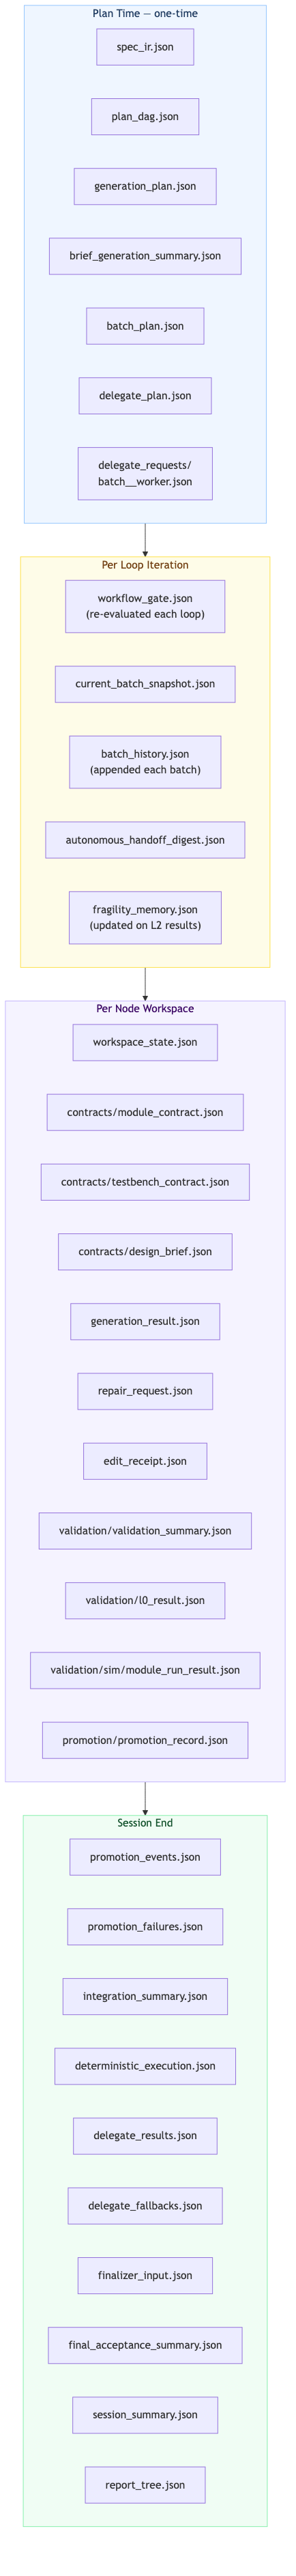
\includegraphics[keepaspectratio,alt={图5-4: JSON构件生命周期}]{../fpga_flow/diagrams/12_json_artifact_lifecycle.png}}
\caption{图5-4: JSON构件生命周期}
\end{figure}

\subsubsection{5.4.4
集成测试与子模块验证的层次关系}\label{ux96c6ux6210ux6d4bux8bd5ux4e0eux5b50ux6a21ux5757ux9a8cux8bc1ux7684ux5c42ux6b21ux5173ux7cfb}

集成回归测试在四层验证体系中处于顶层，与子模块L0/L1/L2验证形成层次关系：子模块验证关注局部行为正确性，集成验证关注系统级行为正确性和模块间交互。

本框架的设计原则是：每个模块在进入集成测试前必须经过独立的L0+L1验证（可选L2），PROMOTED状态是集成测试的前提条件。这一''先分后合''的验证策略减少了集成测试阶段的调试负担，提高了系统整体的验证效率。

四层验证体系的完整执行路径为：

\begin{verbatim}
L0编译门控 → L1仿真+Checkpoint → (L2鲁棒性测试) → 所有模块PROMOTED → 集成回归测试 → DONE
\end{verbatim}

每一层都是下一层的前提，每一层的验证结果都直接驱动框架控制流的状态转移，形成了一套机器自动判定、无需人工干预的完整验证体系。

\section{第六章 Harnessing
Engine：LLM约束引擎设计}\label{ux7b2cux516dux7ae0-harnessing-enginellmux7ea6ux675fux5f15ux64ceux8bbeux8ba1}

\subsection{6.1 Harnessing
Engine概念与架构}\label{harnessing-engineux6982ux5ff5ux4e0eux67b6ux6784}

\subsubsection{6.1.1
问题定义：LLM在硬件设计中的失败模式}\label{ux95eeux9898ux5b9aux4e49llmux5728ux786cux4ef6ux8bbeux8ba1ux4e2dux7684ux5931ux8d25ux6a21ux5f0f}

大语言模型在代码生成任务中展现出令人期待的能力，但同时暴露出若干系统性失败模式。在硬件设计自动化这一高精度、强约束的应用场景中，这些失败模式尤为突出，且具有跨设计对象的共性------无论目标是密码学模块、信号处理
IP 核还是总线控制器，LLM 均可能产生以下五类失败：

\textbf{失败模式一：幻觉端口/信号}。LLM在生成Verilog代码时，可能凭借训练数据中的统计模式''自行发明''实际不存在的端口（如将\texttt{key\_in}改写为\texttt{key\_data}），或在例化子模块时连接错误的端口名称。由于Verilog对未声明信号有时会静默警告而非报错，这类错误可能通过编译但在仿真阶段才暴露。

\textbf{失败模式二：语法错误}。LLM生成的Verilog代码有时包含非法语法结构，如在\texttt{always}块中混用阻塞/非阻塞赋值、在组合逻辑中使用时序敏感列表错误、参数化语法不兼容等。这类错误通常在L0编译门控阶段即可捕获，但若Agent仅修改部分代码而引入新的语法问题，则可能形成''修复一处、引入两处''的循环。

\textbf{失败模式三：Scope
drift（范围漂移）}。Agent在修复单个模块问题时，可能''顺手''修改了其他模块的接口定义或共享头文件，破坏模块间的已冻结接口契约。这类问题在单模块测试中不可见，只有在集成阶段才会暴露。

\textbf{失败模式四：过度修改}。修复Agent面对一个编译错误时，可能大幅重写整个模块而非进行最小化修复，将原本正确的逻辑也一并破坏。这种''推倒重来''模式缺乏收敛保证，可能导致验证状态在REPAIRING和L0\_FAIL之间无限循环。

\textbf{失败模式五：格式错误}。LLM可能输出Markdown代码块包裹的Verilog代码、在RTL文件中夹杂自然语言解释、或将完整JSON文件内容逐字输出到对话中，破坏文件格式和上下文效率。

\subsubsection{6.1.2 Harnessing
Engine设计理念}\label{harnessing-engineux8bbeux8ba1ux7406ux5ff5}

针对上述失败模式，本文提出''Harnessing
Engine''（驾驭引擎）概念，作为一种通用的 LLM
行为约束框架模式。其核心设计理念是：\textbf{不依赖 LLM
自律，通过结构化的外部约束从六个层面系统性地驾驭 LLM 行为}。Harnessing
Engine
的六层架构（Skill/Prompt/Memory/Hooks/MCP/SlashCommand）是领域无关的约束模式------每一层的约束机制均可通过替换领域内容适配不同的硬件设计目标，甚至扩展到软件工程等其他
LLM 应用场景。

``Harnessing''（驾驭）一词的选择具有深刻的工程意涵：驾驭不是压制，而是通过设计良好的约束结构，引导LLM的能力在期望的范围内发挥作用。如同马具（harness）不限制马的力量，而是引导其方向，Harnessing
Engine不试图消除LLM的创造性，而是通过六层约束确保这种创造性不会越出工程规约的边界。

Harnessing Engine的六层约束从架构上形成了一个完整的防御体系：

\begin{figure}
\centering
\pandocbounded{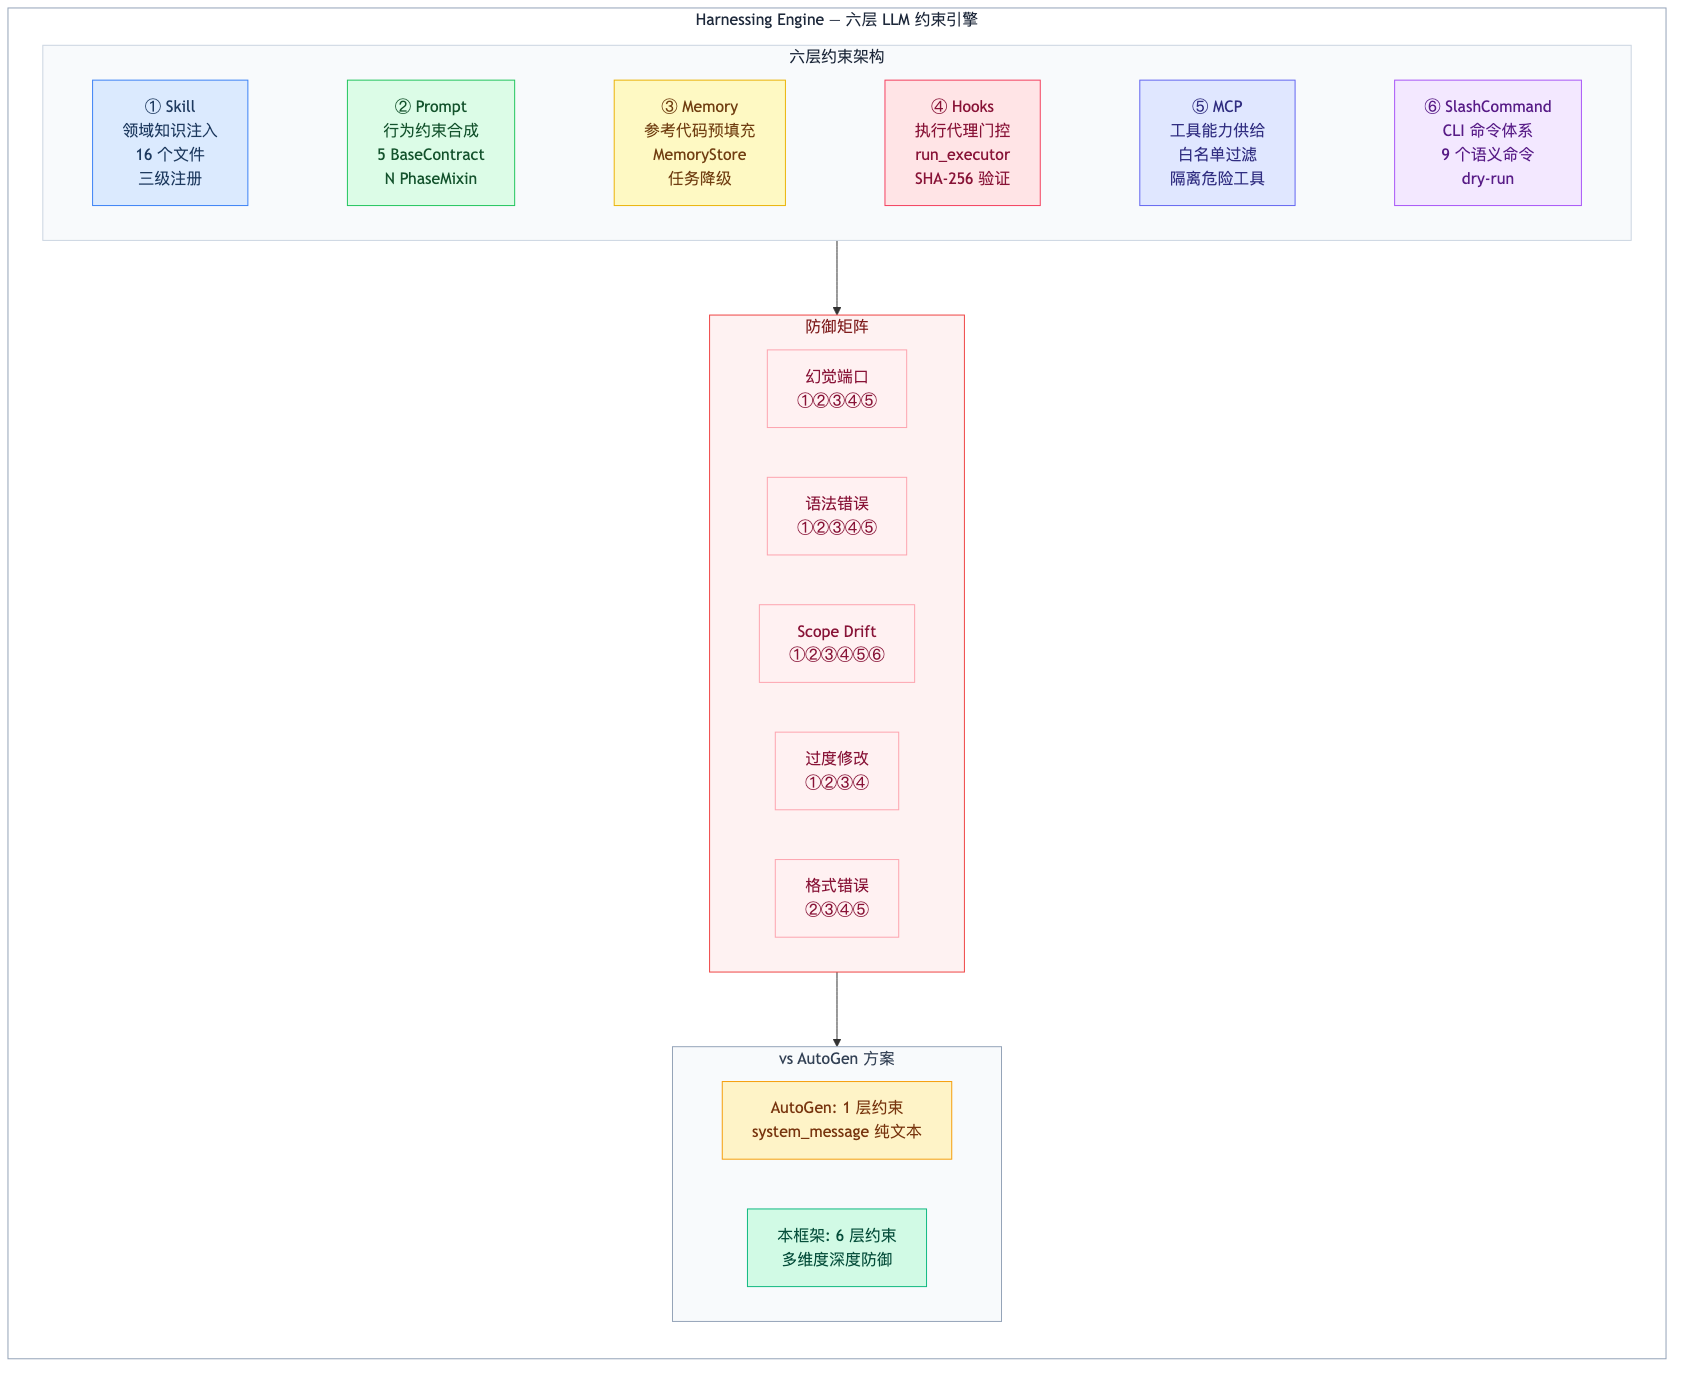
\includegraphics[keepaspectratio,alt={图6-1: Harnessing Engine六层约束架构总览}]{../fpga_flow/diagrams/16_harnessing_engine.png}}
\caption{图6-1: Harnessing Engine六层约束架构总览}
\end{figure}

\begin{figure}
\centering
\pandocbounded{
\includegraphics[keepaspectratio,alt={图6-2: Prompt合成流程}]{../fpga_flow/diagrams/10_prompt_composition.png}}
\caption{图6-2: Prompt合成流程}
\end{figure}

六层约束的分工如下表所示：

{[}表6-1: LLM失败模式-约束层级防御矩阵（详见6.8节）{]}

\begin{center}\rule{0.5\linewidth}{0.5pt}\end{center}

\subsection{6.2
Skill层：领域知识注入}\label{skillux5c42ux9886ux57dfux77e5ux8bc6ux6ce8ux5165}

\subsubsection{6.2.1
三级Skill注册体系}\label{ux4e09ux7ea7skillux6ce8ux518cux4f53ux7cfb}

Skill
层的三级注册体系（运行时/内存/文档）是一种通用的领域知识管理架构。运行时
Skill 注入运行时约束，内存 Skill 提供参考代码，文档 Skill
辅助离线合成。这一三级架构可直接复用于其他硬件设计------替换 Skill
文件内容即可适配新的设计领域。在 AES-128 验证案例中，16 个 Skill
文件按以下方式实例化：

本框架构建了由16个Skill文件组成的三级注册体系，通过\texttt{skill\_refs.py}统一管理。三级注册体系的分工严格区分了运行时注入与离线参考的职责：

\textbf{运行时Skill（Runtime
Skills，5个）}：通过\texttt{get\_runtime\_skill\_refs()}（\texttt{fpga\_flow/skill\_refs.py:22-51}）获取，直接注入到Agent的系统提示词中，在运行时作为硬约束约束Agent行为：

{\def\LTcaptype{none} % do not increment counter
\begin{longtable}[]{@{}
  >{\raggedright\arraybackslash}p{(\linewidth - 4\tabcolsep) * \real{0.4286}}
  >{\raggedright\arraybackslash}p{(\linewidth - 4\tabcolsep) * \real{0.2857}}
  >{\raggedright\arraybackslash}p{(\linewidth - 4\tabcolsep) * \real{0.2857}}@{}}
\toprule\noalign{}
\begin{minipage}[b]{\linewidth}\raggedright
Skill键
\end{minipage} & \begin{minipage}[b]{\linewidth}\raggedright
名称
\end{minipage} & \begin{minipage}[b]{\linewidth}\raggedright
用途
\end{minipage} \\
\midrule\noalign{}
\endhead
\bottomrule\noalign{}
\endlastfoot
\texttt{aes\_verilator\_profile} & aes-verilator-profile &
AES节点分类、向量、Checkpoint、L2约定 \\
\texttt{aes\_module\_patterns} & aes-module-patterns &
S-box、密钥扩展、轮变换、顶层集成的参考模式 \\
\texttt{aes\_tb\_contracts} & aes-tb-contracts & 自检C++
Testbench契约、向量和Checkpoint语义 \\
\texttt{aes\_repair\_heuristics} & aes-repair-heuristics &
编译/Checkpoint/延迟/握手失败的修复启发式规则 \\
\texttt{openhands\_sdk\_subagent\_delegation} &
openhands-sdk-subagent-delegation &
子Agent注册、spawn、委派和任务边界规则 \\
\end{longtable}
}

\textbf{内存Skill（Memory
Skills，5个）}：通过\texttt{get\_memory\_skill\_refs()}（\texttt{fpga\_flow/skill\_refs.py:54-83}）获取，由\texttt{MemoryStore}管理，包含验证通过的AES参考RTL代码，用于工作区预填充：

{\def\LTcaptype{none} % do not increment counter
\begin{longtable}[]{@{}
  >{\raggedright\arraybackslash}p{(\linewidth - 4\tabcolsep) * \real{0.3750}}
  >{\raggedright\arraybackslash}p{(\linewidth - 4\tabcolsep) * \real{0.3750}}
  >{\raggedright\arraybackslash}p{(\linewidth - 4\tabcolsep) * \real{0.2500}}@{}}
\toprule\noalign{}
\begin{minipage}[b]{\linewidth}\raggedright
Skill键
\end{minipage} & \begin{minipage}[b]{\linewidth}\raggedright
对应模块
\end{minipage} & \begin{minipage}[b]{\linewidth}\raggedright
内容
\end{minipage} \\
\midrule\noalign{}
\endhead
\bottomrule\noalign{}
\endlastfoot
\texttt{aes\_memory\_sbox} & aes\_sbox & 验证通过的S-box
RTL+TB参考实现 \\
\texttt{aes\_memory\_key\_schedule} & aes\_key\_schedule\_128 &
验证通过的密钥扩展RTL+TB参考实现 \\
\texttt{aes\_memory\_round\_transform} & aes\_round\_transform &
验证通过的轮变换RTL+TB参考实现 \\
\texttt{aes\_memory\_encrypt\_core} & aes128\_encrypt\_core &
验证通过的顶层加密核RTL+TB参考实现 \\
\texttt{aes\_memory\_shared} & 公共 & aes\_sbox\_lut.vh +
aes\_tb\_common.hpp上下文 \\
\end{longtable}
}

\textbf{文档Skill（Documentation
Skills，6个）}：通过\texttt{get\_documentation\_skill\_refs()}（\texttt{fpga\_flow/skill\_refs.py:86-120}）获取，供\texttt{synthesis.py}中的\texttt{ModuleDesignBrief}生成使用，不注入Agent运行时提示词。

{[}表6-2: 16个Skill文件分类表（名称、类型、用途）{]}

\subsubsection{6.2.2
Skill分组与按角色注入}\label{skillux5206ux7ec4ux4e0eux6309ux89d2ux8272ux6ce8ux5165}

Skill按Agent角色分组，实现精准注入。\texttt{WORKER\_FPGA\_CORE\_SKILL\_KEYS}（\texttt{fpga\_flow/skill\_refs.py:158-163}）包含3个核心Worker技能；\texttt{REPAIR\_CORE\_SKILL\_KEYS}仅包含\texttt{aes\_repair\_heuristics}；\texttt{ORCHESTRATOR\_CORE\_SKILL\_KEYS}仅包含\texttt{aes\_verilator\_profile}。

\texttt{select\_worker\_skill\_keys(active\_mode)}函数根据当前工作模式动态选择技能子集：generate模式使用\texttt{WORKER\_FPGA\_CORE\_SKILL\_KEYS}，repair模式使用\texttt{REPAIR\_CORE\_SKILL\_KEYS}，l2\_execute模式使用\texttt{L2\_WORKER\_SKILL\_KEYS}（仅\texttt{aes\_verilator\_profile}）。这一按模式精准注入的设计减少了提示词的冗余信息，降低了LLM''混淆技能''的可能性。

\subsubsection{6.2.3
SKILLS\_AS\_AUTHORITY\_CONTRACT}\label{skills_as_authority_contract}

\texttt{SKILLS\_AS\_AUTHORITY\_CONTRACT}（\texttt{fpga\_flow/prompt\_contracts.py:72-77}）是Skill层的元约束：

\begin{verbatim}
Repository skills are the authority for FPGA, Verilator, and SDK policy;
do not paraphrase or restate them.
\end{verbatim}

这一约束明确告知Agent：Skill文件是工程策略的权威来源，Agent不得根据自身训练数据''推断''或''改写''技能内容。与AutoGen方案的对比：该方案仅有\texttt{system\_message}中的纯文本指令，无结构化技能体系，Agent可能基于通用训练数据''自行推断''HDL设计规则，而这些推断与项目规约可能存在偏差。

\begin{center}\rule{0.5\linewidth}{0.5pt}\end{center}

\subsection{6.3
Prompt层：行为约束合成}\label{promptux5c42ux884cux4e3aux7ea6ux675fux5408ux6210}

\subsubsection{6.3.1
可组合Prompt架构}\label{ux53efux7ec4ux5408promptux67b6ux6784}

可组合 Prompt 架构（BaseContract + PhaseMixin +
InstancePayload）是一种领域无关的提示词工程模式。BaseContract
定义不可覆盖的硬约束，PhaseMixin 提供阶段适配的补充约束，InstancePayload
注入任务具体参数。这一组合机制使得框架能够为不同设计对象的不同执行阶段精确定制
Agent 行为约束。

本框架的提示词不是单一的静态字符串，而是通过\texttt{compose\_prompt()}函数（\texttt{fpga\_flow/prompt\_contracts.py:32-49}）将四层组件动态组合而成：

\begin{Shaded}
\begin{Highlighting}[]
\KeywordTok{def}\NormalTok{ compose\_prompt(}
\NormalTok{    role\_intro: }\BuiltInTok{str}\NormalTok{,}
    \OperatorTok{*}\NormalTok{,}
\NormalTok{    base\_contracts: Iterable[BaseContract],}
\NormalTok{    phase\_mixins: Iterable[PhaseMixin] }\OperatorTok{=}\NormalTok{ (),}
\NormalTok{    instance\_payload: InstancePayload }\OperatorTok{|} \VariableTok{None} \OperatorTok{=} \VariableTok{None}\NormalTok{,}
\NormalTok{    skill\_block: }\BuiltInTok{str} \OperatorTok{|} \VariableTok{None} \OperatorTok{=} \VariableTok{None}\NormalTok{,}
\NormalTok{) }\OperatorTok{{-}\textgreater{}} \BuiltInTok{str}\NormalTok{:}
\end{Highlighting}
\end{Shaded}

四层组件的职责划分如下：

\begin{figure}
\centering
\pandocbounded{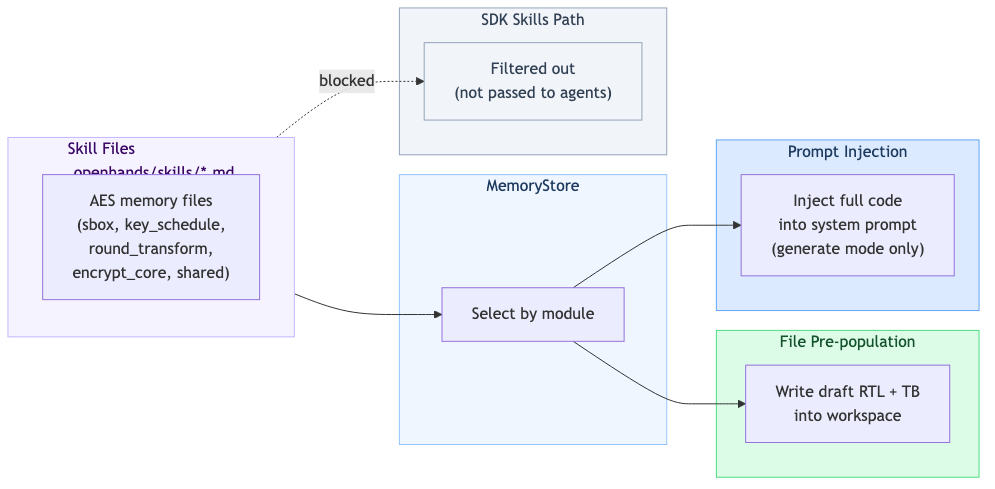
\includegraphics[keepaspectratio,alt={图6-3: Memory注入流程}]{../fpga_flow/diagrams/07_memory_injection.png}}
\caption{图6-3: Memory注入流程}
\end{figure}

\textbf{第一层：角色引言（role\_intro）}：声明Agent的身份和职责范围，如\texttt{You\ are\ the\ Module\ Worker\ SubAgent\ for\ aes\_sbox.}，确立了任务局部性。

\textbf{第二层：基础合约（BaseContract）}：硬约束集合，在所有工作模式下均有效，不可覆盖。5个核心BaseContract的约束维度各异：

{\def\LTcaptype{none} % do not increment counter
\begin{longtable}[]{@{}
  >{\raggedright\arraybackslash}p{(\linewidth - 4\tabcolsep) * \real{0.4000}}
  >{\raggedright\arraybackslash}p{(\linewidth - 4\tabcolsep) * \real{0.3000}}
  >{\raggedright\arraybackslash}p{(\linewidth - 4\tabcolsep) * \real{0.3000}}@{}}
\toprule\noalign{}
\begin{minipage}[b]{\linewidth}\raggedright
BaseContract
\end{minipage} & \begin{minipage}[b]{\linewidth}\raggedright
约束维度
\end{minipage} & \begin{minipage}[b]{\linewidth}\raggedright
核心条款
\end{minipage} \\
\midrule\noalign{}
\endhead
\bottomrule\noalign{}
\endlastfoot
AES\_SCOPE\_CONTRACT & 范围锁定 &
AES-128加密专用，encrypt-only，block-handshake \\
STRUCTURED\_IO\_CONTRACT & IO规范 &
以契约JSON为信息源，禁止cat完整大型JSON文件 \\
NO\_RAW\_VERILATOR\_CONTRACT & 工具隔离 &
禁止直接调用verilator\_compile或verilator\_simulate \\
FRAMEWORK\_OWNS\_PROGRESS\_CONTRACT & 控制权归属 &
框架而非Agent拥有批次推进和工作流完成权 \\
SKILLS\_AS\_AUTHORITY\_CONTRACT & 权威源 &
Skill文件是FPGA/Verilator/SDK策略的权威 \\
\end{longtable}
}

\textbf{第三层：阶段混入（PhaseMixin）}：针对当前执行阶段的补充约束，随工作模式动态切换。例如，\texttt{REPAIR\_PHASE\_ROUND\_1}要求''第一个工具调用必须是对primary\_target\_file的file\_editor
edit''，强制Agent先编辑后验证，防止无效的信息收集操作浪费修复轮次预算。

\textbf{第四层：实例负载（InstancePayload）}：当前任务的具体参数，如可写文件列表、Campaign参数、特殊行为注记等。

\subsubsection{6.3.2
PhaseMixin的阶段适配机制}\label{phasemixinux7684ux9636ux6bb5ux9002ux914dux673aux5236}

本框架在Prompt构建中对\textbf{非修复模式}与\textbf{修复模式}采用了完全不同的函数路径，这是有意为之的架构分离设计。

\textbf{非修复模式：\texttt{\_select\_phase\_mixins(active\_mode)}}（\texttt{fpga\_flow/prompts.py:91-114}）

该函数处理\texttt{generate}、\texttt{validate}、\texttt{l2\_execute}三种模式，由\texttt{build\_module\_worker\_prompt()}调用：

\begin{itemize}
\tightlist
\item
  \texttt{generate}模式：在基础混入（\texttt{WORKER\_LOCAL\_SCOPE}、\texttt{WORKER\_REQUEST\_AUTHORITY}、\texttt{RUN\_EXECUTOR\_PHASE}）之上加入\texttt{GENERATE\_PHASE}和\texttt{MEMORY\_CONSULTATION\_DIRECTIVE}
\item
  \texttt{validate}模式：在基础混入之上加入\texttt{VALIDATE\_PHASE}和\texttt{MEMORY\_CONSULTATION\_DIRECTIVE}（读多写少）
\item
  \texttt{l2\_execute}模式：在基础混入之上加入\texttt{L2\_PHASE}（禁止RTL/TB编辑）
\end{itemize}

\textbf{关键约束}：若\texttt{active\_mode=\textquotesingle{}repair\textquotesingle{}}传入\texttt{\_select\_phase\_mixins()}，函数会\textbf{抛出\texttt{ValueError}}（\texttt{fpga\_flow/prompts.py:97-101}），明确禁止通过此路径构建修复Prompt：

\begin{Shaded}
\begin{Highlighting}[]
\ControlFlowTok{elif}\NormalTok{ active\_mode }\OperatorTok{==} \StringTok{\textquotesingle{}repair\textquotesingle{}}\NormalTok{:}
    \ControlFlowTok{raise} \PreprocessorTok{ValueError}\NormalTok{(}
        \StringTok{\textquotesingle{}Use build\_repair\_worker\_prompt() for repair mode, \textquotesingle{}}
        \StringTok{"not build\_module\_worker\_prompt(active\_mode=\textquotesingle{}repair\textquotesingle{})"}
\NormalTok{    )}
\end{Highlighting}
\end{Shaded}

\textbf{修复模式：\texttt{build\_repair\_worker\_prompt()}}（\texttt{fpga\_flow/prompts.py:198-226}）

修复工作器使用完全独立的Prompt构建函数，不经过\texttt{\_select\_phase\_mixins()}。该函数根据修复轮次选择阶段混入：

\begin{itemize}
\tightlist
\item
  \texttt{repair\_round\ \textless{}=\ 1}：使用\texttt{REPAIR\_PHASE\_ROUND\_1}（编辑优先协议------第一个工具调用必须是对\texttt{primary\_target\_file}的文件编辑，基于\texttt{repair\_request.json}中已提供的文件摘录直接修复，无需重新读文件）
\item
  \texttt{repair\_round\ \textgreater{}\ 1}：使用\texttt{REPAIR\_PHASE\_ROUND\_2\_PLUS}（允许先查看当前文件状态------先前的编辑可能已改变文件内容，Agent需以磁盘状态为准进行针对性修复）
\end{itemize}

修复Prompt还固定注入\texttt{WORKER\_LOCAL\_SCOPE}和\texttt{REPAIR\_MEMORY\_DIRECTIVE}，但\textbf{不注入Memory
Block}------修复阶段的草稿文件可能已经过多轮修改，原始参考记忆已不反映当前磁盘状态。

这一架构分离的设计意图是：修复工作器与生成/验证工作器在行为约束上有本质差异，强制使用独立入口可以防止在修复路径中意外注入生成阶段的约束（如\texttt{MEMORY\_CONSULTATION\_DIRECTIVE}中对参考记忆的依赖），确保修复行为始终以当前磁盘状态为基准。

\subsubsection{6.3.3
典型反幻觉指令}\label{ux5178ux578bux53cdux5e7bux89c9ux6307ux4ee4}

Prompt层包含若干针对特定幻觉模式的反幻觉指令：

\begin{itemize}
\tightlist
\item
  \texttt{"Never\ cat\ whole\ large\ JSON\ files;\ use\ bounded\ reads\ only"}
  --- 防止Agent将整个工作区JSON文件内容输出到对话，导致上下文溢出
\item
  \texttt{"first\ tool\ call\ MUST\ be\ a\ file\_editor\ edit\ on\ primary\_target\_file"}
  --- 防止修复Agent在预算有限的情况下浪费调用次数在信息收集上
\item
  \texttt{"Do\ not\ change\ cross-module\ architecture,\ frozen\ interfaces,\ or\ integration\ policy"}
  --- 防止Scope drift
\item
  \texttt{"Do\ not\ broadly\ scan\ unrelated\ paths\ before\ consulting\ the\ task\ contract"}
  --- 防止Agent在任务开始时进行无边界的文件系统探索
\end{itemize}

\begin{center}\rule{0.5\linewidth}{0.5pt}\end{center}

\subsection{6.4
Memory层：验证代码预填充}\label{memoryux5c42ux9a8cux8bc1ux4ee3ux7801ux9884ux586bux5145}

\subsubsection{6.4.1
MemoryStore核心机制}\label{memorystoreux6838ux5fc3ux673aux5236}

Memory
层的核心机制------将验证通过的参考代码预填充到工作区------是一种通用的
LLM 任务降级策略。通过提供高质量参考实现，Agent
的任务从''从零生成正确代码''降级为''基于参考实现解决集成问题''，显著降低了出错概率。这一策略适用于任何拥有参考实现库的硬件设计领域。在
AES-128 验证案例中，\texttt{MemoryStore} 管理 4 个模块的参考 RTL 和
Testbench。

\texttt{MemoryStore}（\texttt{fpga\_flow/memory.py:57-174}）是AES参考内存检索的单一信息源，封装了从Skill文件中提取验证通过代码的完整逻辑。其核心注册表为\texttt{\_MEMORY\_REGISTRY}（\texttt{fpga\_flow/memory.py:18-23}）：

\begin{Shaded}
\begin{Highlighting}[]
\NormalTok{\_MEMORY\_REGISTRY: }\BuiltInTok{dict}\NormalTok{[}\BuiltInTok{str}\NormalTok{, }\BuiltInTok{str}\NormalTok{] }\OperatorTok{=}\NormalTok{ \{}
    \StringTok{\textquotesingle{}aes\_sbox\textquotesingle{}}\NormalTok{: }\StringTok{\textquotesingle{}aes\_memory\_sbox\textquotesingle{}}\NormalTok{,}
    \StringTok{\textquotesingle{}aes\_key\_schedule\_128\textquotesingle{}}\NormalTok{: }\StringTok{\textquotesingle{}aes\_memory\_key\_schedule\textquotesingle{}}\NormalTok{,}
    \StringTok{\textquotesingle{}aes\_round\_transform\textquotesingle{}}\NormalTok{: }\StringTok{\textquotesingle{}aes\_memory\_round\_transform\textquotesingle{}}\NormalTok{,}
    \StringTok{\textquotesingle{}aes128\_encrypt\_core\textquotesingle{}}\NormalTok{: }\StringTok{\textquotesingle{}aes\_memory\_encrypt\_core\textquotesingle{}}\NormalTok{,}
\NormalTok{\}}
\end{Highlighting}
\end{Shaded}

每个\texttt{module\_id}映射到对应的内存Skill键，Skill文件中包含经过Verilator验证的RTL
Verilog和C++
Testbench代码，通过Markdown代码块（\texttt{verilog\textasciigrave{}和}cpp\texttt{）标记。}\_extract\_code\_block()\texttt{函数（}fpga\_flow/memory.py:39-44`）使用正则表达式提取特定语言的代码块内容。

\subsubsection{6.4.2
两种使用模式}\label{ux4e24ux79cdux4f7fux7528ux6a21ux5f0f}

Memory层提供两种互补的使用模式：

\textbf{\texttt{populate\_workspace()}}（\texttt{fpga\_flow/memory.py:114-159}）：生成模式。将参考代码写入工作区\texttt{draft/rtl/\textless{}module\_id\textgreater{}.v}和\texttt{draft/tb/\textless{}module\_id\textgreater{}\_tb.cpp}文件。写入采用''仅在不存在时写入''的策略（\texttt{if\ not\ rtl\_path.exists():\ rtl\_path.write\_text(...)}），防止覆盖Agent已进行的修改。若内存提取失败（RTL或TB为None），则抛出\texttt{RuntimeError}，这是一个硬错误------框架不允许在无参考实现的情况下进入生成阶段。

\textbf{\texttt{build\_prompt\_block()}}（\texttt{fpga\_flow/memory.py:97-112}）：提示词注入模式。将参考代码以\texttt{===\ MEMORY:\ \textless{}name\textgreater{}\ ===}块的形式直接注入Agent系统提示词，使Agent在生成模式下能够''看到''参考实现：

\begin{verbatim}
=== MEMORY: aes-memory-sbox ===
[skill文件内容，含验证通过的Verilog和C++代码]
=== END MEMORY ===
\end{verbatim}

这一设计的核心洞察是：\textbf{将Agent的任务从''从零生成正确代码''降级为''基于参考实现解决集成问题''}。从零生成正确的AES
RTL代码需要LLM同时掌握AES算法、Verilog语法、Verilator兼容性规约和Checkpoint协议，任何一项理解偏差都会导致失败。而基于参考实现进行适应性修改，Agent只需关注当前任务的具体差异，显著降低了出错概率。

\subsubsection{6.4.3
MEMORY\_CONSULTATION\_DIRECTIVE与REPAIR\_MEMORY\_DIRECTIVE的区分}\label{memory_consultation_directiveux4e0erepair_memory_directiveux7684ux533aux5206}

两个Memory相关的PhaseMixin体现了不同阶段的内存使用策略：

\texttt{MEMORY\_CONSULTATION\_DIRECTIVE}（\texttt{fpga\_flow/prompt\_contracts.py:185-194}）用于generate/validate模式：

\begin{verbatim}
Your workspace draft files are pre-populated from verified AES reference memory.
The === MEMORY === blocks in your system prompt contain the same code that was
written to your draft files. The reference code passes all Verilator checkpoints.
You may reproduce it verbatim or adapt it.
\end{verbatim}

\texttt{REPAIR\_MEMORY\_DIRECTIVE}（\texttt{fpga\_flow/prompt\_contracts.py:196-204}）用于repair模式：

\begin{verbatim}
Your workspace draft files were originally pre-populated from verified AES reference
memory. The on-disk draft files are the current truth — they may have been modified
by prior repair rounds. Do not assume the original reference memory matches the
current file state. Always read the actual file before editing.
\end{verbatim}

这一区分防止了修复Agent基于''记忆中的参考实现''而非''磁盘上的当前状态''进行修复，避免了修复轮次之间状态不一致的问题。

\begin{center}\rule{0.5\linewidth}{0.5pt}\end{center}

\subsection{6.5
Hooks层：执行回调与门控}\label{hooksux5c42ux6267ux884cux56deux8c03ux4e0eux95e8ux63a7}

\subsubsection{6.5.1
run\_executor自定义工具}\label{run_executorux81eaux5b9aux4e49ux5de5ux5177}

run\_executor 自定义工具的代理模式适用于任何硬件设计------Agent
通过统一的工具接口触发编译和仿真，无需了解底层 EDA 工具的命令行细节。

\texttt{run\_executor}（\texttt{fpga\_flow/runtime/execution\_tools.py:30-147}）是本框架最重要的约束机制之一，也是Agent触发框架执行动作的唯一合法入口。其设计核心是：\textbf{通过单一受控工具替代多个原始工具，在Agent和底层EDA工具之间建立强制性的代理层}。

\texttt{run\_executor}的执行流程：

\begin{enumerate}
\def\labelenumi{\arabic{enumi}.}
\tightlist
\item
  Agent调用\texttt{run\_executor(request\_path=\textless{}task\_contract.json\textgreater{})}
\item
  \texttt{\_load\_task\_contract()}从路径读取并验证任务合约JSON（\texttt{DelegateBatchTask}
  Pydantic模型）
\item
  \texttt{\_infer\_executor\_kind()}根据任务模式推断执行器类型（GENERATE\_NODE、RUN\_NODE、RECORD\_REPAIR\_EDIT）
\item
  调度对应的执行器（\texttt{L0Executor}、\texttt{L1Executor}、\texttt{L2CampaignExecutor}、\texttt{IntegrationRegressionExecutor}）
\item
  返回\texttt{RunExecutorObservation}，包含执行状态、结果路径和下一步读取提示
\end{enumerate}

\subsubsection{6.5.2
RunExecutorObservation的引导性设计}\label{runexecutorobservationux7684ux5f15ux5bfcux6027ux8bbeux8ba1}

\texttt{RunExecutorObservation}（\texttt{fpga\_flow/runtime/execution\_tools.py:39-116}）不仅是执行结果的载体，还是Agent下一步行为的引导者。\texttt{next\_read\_paths}字段明确告知Agent执行结束后应读取哪些文件；\texttt{next\_read\_hints}中的\texttt{NextReadHints}包含\texttt{action}（READ\_ARTIFACTS、EDIT\_PRIMARY\_TARGET、WAIT\_FOR\_NEXT\_BATCH、ESCALATE\_TO\_ORCHESTRATOR）和\texttt{reason}字段，将框架的判断意图以结构化方式传达给Agent。

这一设计的意义在于：Agent接收到\texttt{run\_executor}的返回值后，不需要根据自身判断决定下一步查看什么文件或采取什么行动，而是遵循框架通过\texttt{next\_read\_hints}提供的明确指示，大幅减少了Agent决策的不确定性。

\subsubsection{6.5.3
verify\_repair\_edit哈希验证}\label{verify_repair_editux54c8ux5e0cux9a8cux8bc1}

\texttt{verify\_repair\_edit()}（\texttt{fpga\_flow/generation.py:680-735}）是Hooks层的另一核心机制，用于机器化验证修复编辑的真实性。其验证逻辑包含两个独立条件：

\textbf{条件一：文件哈希变化验证}。框架在写入修复请求前记录\texttt{primary\_target\_file}的SHA256哈希值（存入\texttt{repair\_contract.edit\_verification{[}\textquotesingle{}baseline\_hashes\textquotesingle{}{]}}），修复后对比当前哈希。若哈希未变化，说明Agent声称已修复但实际未修改文件，验证失败并拒绝推进至重新验证阶段。

\textbf{条件二：必要Token存在验证}。\texttt{repair\_contract.must\_add\_tokens}列出修复后文件必须包含的token（如\texttt{CHECKPOINT\textbar{}CHK\_XXX\textbar{}PASS\textbar{}}），框架验证这些token确实出现在修改后的文件中。验证器还接受等价形式：若token以\texttt{CHECKPOINT\textbar{}}开头，则\texttt{emit\_checkpoint("CHK\_XXX",\ ...)}调用也被视为满足要求。

这一双重验证机制彻底消除了Agent''虚假声称修复成功''的可能性------没有真实的文件修改和必要代码的添加，框架不会进入重新验证阶段。

\subsubsection{6.5.4 Batch
Gate回调机制}\label{batch-gateux56deux8c03ux673aux5236}

框架通过文件系统轮询实现Batch
Gate，将文件系统作为Agent和框架之间的通信通道：Agent将执行结果写入工作区文件（如\texttt{validation\_summary.json}、\texttt{module\_run\_result.json}），框架的\texttt{run\_current\_batch\_until\_gate()}定期轮询这些文件，判断批次完成条件。当所有节点均有结果文件产生且状态满足门控条件时，框架结束当前批次，推进到下一状态。

\begin{center}\rule{0.5\linewidth}{0.5pt}\end{center}

\subsection{6.6
MCP层：工具能力供给}\label{mcpux5c42ux5de5ux5177ux80fdux529bux4f9bux7ed9}

\subsubsection{6.6.1 Model Context
Protocol的角色}\label{model-context-protocolux7684ux89d2ux8272}

MCP 工具过滤机制是通用的，可根据不同场景配置排除列表。

Model Context Protocol（MCP）是AI
Agent与外部工具之间的标准化通信协议。在本框架中，MCP承担着连接LLM
Agent与Verilator
EDA工具链的桥梁角色，将复杂的Verilator命令行接口封装为Agent可调用的结构化工具接口。

\begin{figure}
\centering
\pandocbounded{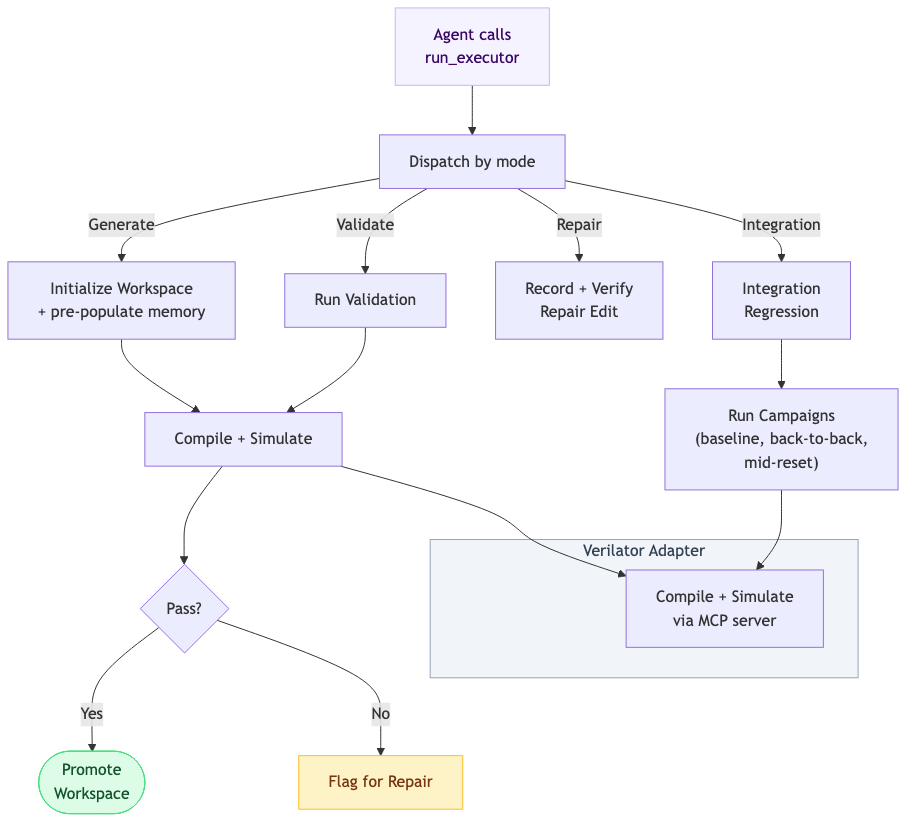
\includegraphics[keepaspectratio,alt={图6-4: 执行器调度流程}]{../fpga_flow/diagrams/08_executor_dispatch.png}}
\caption{图6-4: 执行器调度流程}
\end{figure}

\begin{figure}
\centering
\pandocbounded{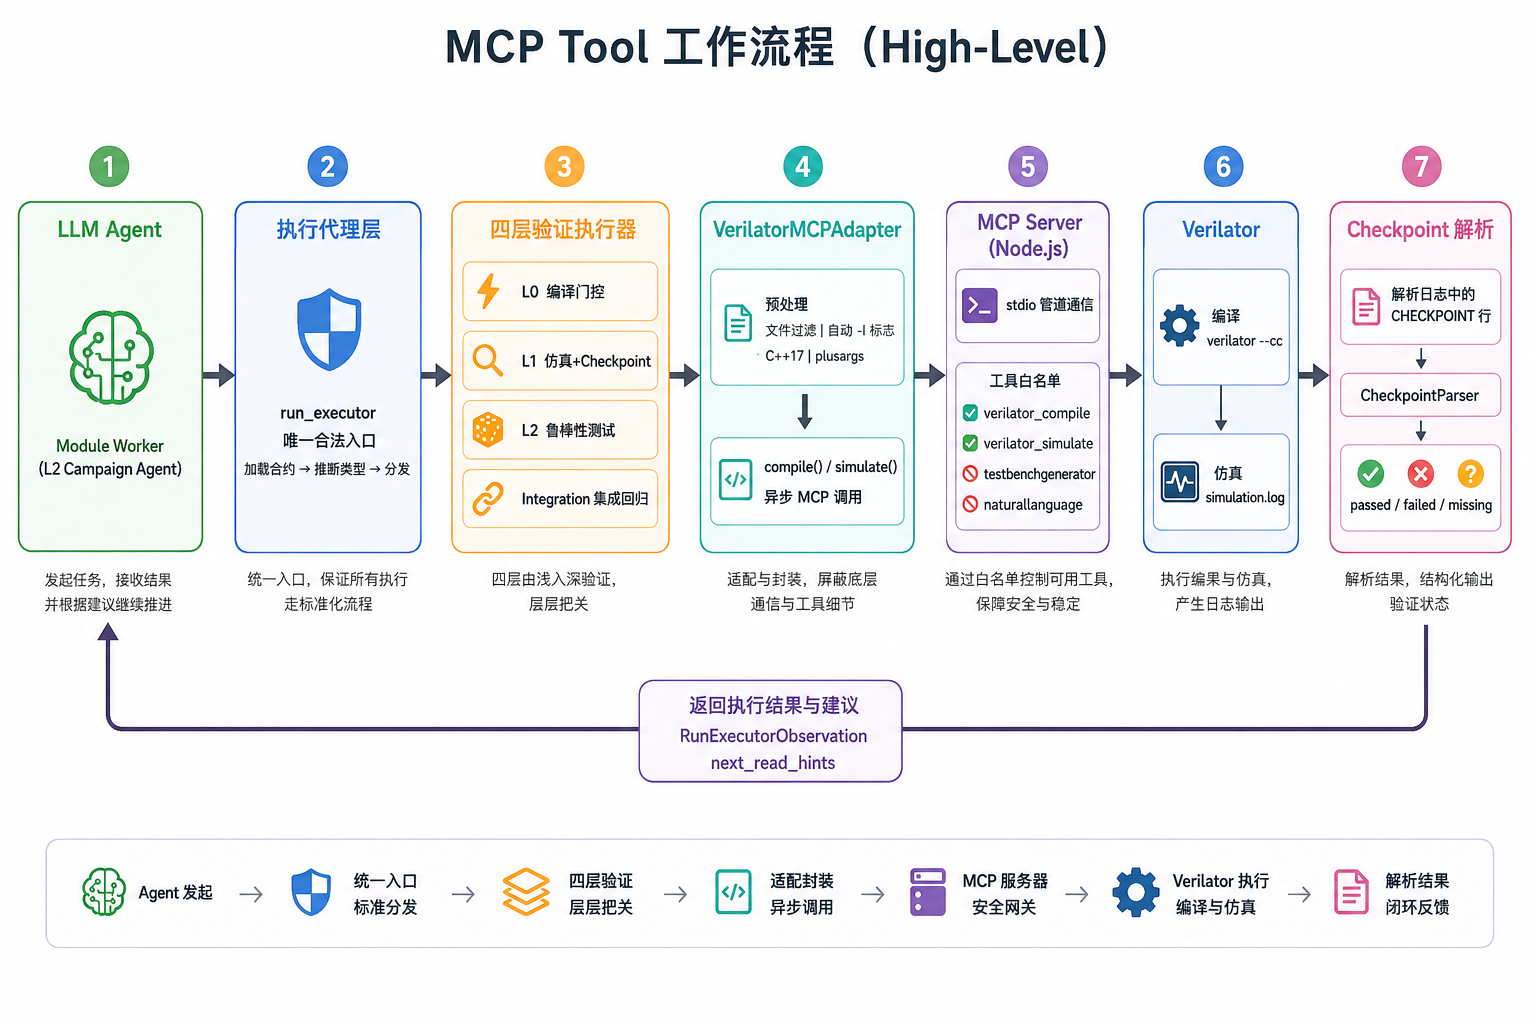
\includegraphics[keepaspectratio,alt={图6-5: MCP Verilator适配器架构}]{../fpga_flow/diagrams/15_mcp_verilator_adapter.png}}
\caption{图6-5: MCP Verilator适配器架构}
\end{figure}

\subsubsection{6.6.2
VerilatorMCPAdapter封装细节}\label{verilatormcpadapterux5c01ux88c5ux7ec6ux8282}

\texttt{VerilatorMCPAdapter}（\texttt{fpga\_flow/adapters/verilator.py:122-216}）封装了所有与Verilator
MCP服务器的通信细节，对上层执行器（L0/L1/L2/Integration
Executor）提供简洁的\texttt{compile()}和\texttt{simulate()}异步接口。其关键封装逻辑包括：

\textbf{输入文件过滤}：\texttt{\_filter\_verilator\_input\_files()}（\texttt{fpga\_flow/adapters/verilator.py:81-91}）过滤掉目录路径和非标准扩展名文件，只保留\texttt{.v}/\texttt{.sv}（Verilog源文件）和\texttt{.cpp}/\texttt{.cc}/\texttt{.cxx}（C++
Testbench）。这防止了Agent传入不合法文件路径导致Verilator报错。

\textbf{include标志自动生成}：\texttt{\_verilog\_include\_directories()}自动提取Verilog源文件的父目录，生成\texttt{-I/path/to/rtl}格式的include标志，确保\texttt{\textasciigrave{}include\ "aes\_sbox\_lut.vh"}等头文件引用能够正确解析。

\textbf{C++17标准自动添加}：当编译文件列表中包含C++源文件时，自动在\texttt{verilatorFlags}中添加\texttt{-CFLAGS\ -std=c++17}，无需Agent手动指定编译选项。

\textbf{plusargs传递}：\texttt{fpga\_flow\_package\_root}等运行时参数通过Verilator
plusargs机制传递给Testbench，Testbench通过\texttt{resolve\_path(argc,\ argv,\ requested,\ fallback)}函数读取，实现了向量文件的路径无关解析。

\subsubsection{6.6.3
MCP工具过滤：防止Agent绕过框架}\label{mcpux5de5ux5177ux8fc7ux6ee4ux9632ux6b62agentux7ed5ux8fc7ux6846ux67b6}

\texttt{build\_verilator\_stdio\_server()}（\texttt{fpga\_flow/adapters/verilator.py:43-74}）配置MCP服务器时，框架在更高层（\texttt{SdkAgentFactory}）过滤掉两个MCP工具：\texttt{verilator\_testbenchgenerator}和\texttt{verilator\_naturallanguage}。这一过滤的设计意图是：

\begin{itemize}
\tightlist
\item
  \textbf{禁用testbenchgenerator}：防止Agent绕过框架的C++自检Testbench体系，使用自动生成的Testbench（自动Testbench无法实现Checkpoint协议）
\item
  \textbf{禁用naturallanguage}：防止Agent以自然语言描述方式调用Verilator，绕过框架的结构化执行路径
\end{itemize}

这两个工具的禁用体现了MCP层的核心约束原则：Agent只能使用框架明确授权的工具子集，任何可能绕过约束体系的工具入口均被封闭。

\begin{center}\rule{0.5\linewidth}{0.5pt}\end{center}

\subsection{6.7
SlashCommand层：用户交互接口}\label{slashcommandux5c42ux7528ux6237ux4ea4ux4e92ux63a5ux53e3}

\subsubsection{6.7.1 CLI命令体系}\label{cliux547dux4ee4ux4f53ux7cfb}

CLI 命令体系的语义设计面向通用硬件设计验证流程。

\texttt{\_\_main\_\_.py}（\texttt{fpga\_flow/\_\_main\_\_.py}）实现了完整的CLI命令体系，每个命令对应一套完整的验证/执行语义：

\begin{Shaded}
\begin{Highlighting}[]
\ExtensionTok{python} \AttributeTok{{-}m}\NormalTok{ MultiAgent\_FPGA.fpga\_flow validate           }\CommentTok{\# 契约验证（无需API密钥）}
\ExtensionTok{python} \AttributeTok{{-}m}\NormalTok{ MultiAgent\_FPGA.fpga\_flow smoke{-}sdk           }\CommentTok{\# SDK烟测}
\ExtensionTok{python} \AttributeTok{{-}m}\NormalTok{ MultiAgent\_FPGA.fpga\_flow smoke{-}provider      }\CommentTok{\# DeepSeek API预检}
\ExtensionTok{python} \AttributeTok{{-}m}\NormalTok{ MultiAgent\_FPGA.fpga\_flow run{-}node }\OperatorTok{\textless{}}\NormalTok{module}\OperatorTok{\textgreater{}}   \CommentTok{\# 单节点L0+L1验证}
\ExtensionTok{python} \AttributeTok{{-}m}\NormalTok{ MultiAgent\_FPGA.fpga\_flow generate{-}node }\OperatorTok{\textless{}}\NormalTok{module}\OperatorTok{\textgreater{}}  \CommentTok{\# 工作区初始化+验证}
\ExtensionTok{python} \AttributeTok{{-}m}\NormalTok{ MultiAgent\_FPGA.fpga\_flow record{-}repair{-}edit }\OperatorTok{\textless{}}\NormalTok{module}\OperatorTok{\textgreater{}}  \CommentTok{\# 记录修复编辑}
\ExtensionTok{python} \AttributeTok{{-}m}\NormalTok{ MultiAgent\_FPGA.fpga\_flow run{-}integration     }\CommentTok{\# 集成回归测试}
\ExtensionTok{python} \AttributeTok{{-}m}\NormalTok{ MultiAgent\_FPGA.fpga\_flow run{-}aes{-}mvp         }\CommentTok{\# 全流程自主执行}
\ExtensionTok{python} \AttributeTok{{-}m}\NormalTok{ MultiAgent\_FPGA.fpga\_flow run{-}aes{-}mvp }\AttributeTok{{-}{-}dry{-}run}  \CommentTok{\# 干运行（仅规划，不执行）}
\end{Highlighting}
\end{Shaded}

\subsubsection{6.7.2
命令即合约的设计原则}\label{ux547dux4ee4ux5373ux5408ux7ea6ux7684ux8bbeux8ba1ux539fux5219}

每个CLI命令背后是完整的语义定义：\texttt{run-node}命令不仅调用执行器，还管理工作区状态（初始化、验证、修复预算检查）、生成报告文件、更新工作区记录；\texttt{record-repair-edit}命令先运行\texttt{verify\_repair\_edit()}验证修复真实性，再调用\texttt{write\_edit\_receipt()}写入编辑收据，为后续重新验证提供可追溯的审计链。

\texttt{-\/-dry-run}选项实现了规划与执行的分离：框架完成全部初始化（bootstrap、SpecIR/PlanDAG/Manifest合成、Policy验证），但仅输出将要执行的批次计划而不实际调用LLM
API，供用户在正式运行前检查执行策略。

\begin{center}\rule{0.5\linewidth}{0.5pt}\end{center}

\subsection{6.8
六层协同：约束覆盖矩阵}\label{ux516dux5c42ux534fux540cux7ea6ux675fux8986ux76d6ux77e9ux9635}

\subsubsection{6.8.1
LLM失败模式-约束层级防御矩阵}\label{llmux5931ux8d25ux6a21ux5f0f-ux7ea6ux675fux5c42ux7ea7ux9632ux5fa1ux77e9ux9635}

六层约束并非相互独立，而是形成了对LLM失败模式的多层防御体系。下表展示了每种失败模式由哪些约束层级防御：

{[}表6-3: LLM失败模式-约束层级防御矩阵{]}

{\def\LTcaptype{none} % do not increment counter
\begin{longtable}[]{@{}
  >{\raggedright\arraybackslash}p{(\linewidth - 12\tabcolsep) * \real{0.1429}}
  >{\raggedright\arraybackslash}p{(\linewidth - 12\tabcolsep) * \real{0.1270}}
  >{\raggedright\arraybackslash}p{(\linewidth - 12\tabcolsep) * \real{0.1429}}
  >{\raggedright\arraybackslash}p{(\linewidth - 12\tabcolsep) * \real{0.1429}}
  >{\raggedright\arraybackslash}p{(\linewidth - 12\tabcolsep) * \real{0.1270}}
  >{\raggedright\arraybackslash}p{(\linewidth - 12\tabcolsep) * \real{0.0952}}
  >{\raggedright\arraybackslash}p{(\linewidth - 12\tabcolsep) * \real{0.2222}}@{}}
\toprule\noalign{}
\begin{minipage}[b]{\linewidth}\raggedright
失败模式
\end{minipage} & \begin{minipage}[b]{\linewidth}\raggedright
Skill层
\end{minipage} & \begin{minipage}[b]{\linewidth}\raggedright
Prompt层
\end{minipage} & \begin{minipage}[b]{\linewidth}\raggedright
Memory层
\end{minipage} & \begin{minipage}[b]{\linewidth}\raggedright
Hooks层
\end{minipage} & \begin{minipage}[b]{\linewidth}\raggedright
MCP层
\end{minipage} & \begin{minipage}[b]{\linewidth}\raggedright
SlashCommand层
\end{minipage} \\
\midrule\noalign{}
\endhead
\bottomrule\noalign{}
\endlastfoot
\textbf{幻觉端口/信号} &
\texttt{aes\_module\_patterns}提供正确端口规范；\texttt{aes\_verilator\_profile}明确模块接口
&
\texttt{AES\_SCOPE\_CONTRACT}范围锁定；\texttt{WORKER\_REQUEST\_AUTHORITY}以合约为信息源
&
\texttt{populate\_workspace()}写入正确端口的参考RTL；\texttt{build\_prompt\_block()}内联参考实现
& L0编译门控捕获端口连接错误 & Verilator编译器严格验证端口声明 &
\texttt{validate}命令预检契约完整性 \\
\textbf{语法错误} &
\texttt{verilog\_verilator}提供Verilator合规Verilog规则；\texttt{aes\_tb\_contracts}提供合规TB模式
& \texttt{STRUCTURED\_IO\_CONTRACT}约束输出格式 &
参考实现本身是语法正确的Verilog代码 &
L0编译门控精确定位语法错误行；\texttt{RunExecutorObservation.next\_read\_hints}引导读取编译日志
& Verilator编译器是语法权威；自动添加\texttt{-CFLAGS\ -std=c++17} &
\texttt{run-node}命令明确L0失败含义 \\
\textbf{Scope drift} &
\texttt{openhands\_sdk\_subagent\_delegation}明确任务边界规则 &
\texttt{WORKER\_LOCAL\_SCOPE}限制可写范围；\texttt{ORCHESTRATOR\_ONLY\_CURRENT\_BATCH}限制批次范围
& \texttt{populate\_workspace()}只写入当前模块的draft目录 &
\texttt{run\_executor}只接受当前任务合约路径；\texttt{verify\_repair\_edit()}只验证primary\_target\_file
& 工具过滤禁用可能越界的工具 &
每个命令的workspace\_root参数限制操作范围 \\
\textbf{过度修改} &
\texttt{aes\_repair\_heuristics}提供最小化修复启发式规则 &
\texttt{REPAIR\_PHASE\_ROUND\_1}要求首次编辑仅针对primary\_target\_file；禁止secondary\_target\_files的预读
& \texttt{REPAIR\_MEMORY\_DIRECTIVE}要求以磁盘状态为准，不基于记忆重写 &
\texttt{verify\_repair\_edit()}双重验证（哈希+token）；修复预算限制（默认2次）
& --- & \texttt{record-repair-edit}命令强制显式编辑记录 \\
\textbf{格式错误} & --- & \texttt{STRUCTURED\_IO\_CONTRACT}：``Never cat
whole large JSON files''；以合约JSON为信息源 &
内存注入使用\texttt{===\ MEMORY\ ===}块而非原始文件内容 &
\texttt{RunExecutorObservation.to\_llm\_content}将执行结果序列化为结构化文本行
& MCP结果通过\texttt{\_extract\_text\_from\_result()}提取纯文本 &
CLI命令输出格式化JSON报告 \\
\end{longtable}
}

\subsubsection{6.8.2 一个Module
Worker的完整约束链路}\label{ux4e00ux4e2amodule-workerux7684ux5b8cux6574ux7ea6ux675fux94feux8def}

以\texttt{aes\_sbox}模块的generate阶段为例，展示六层约束的协同工作：

\begin{enumerate}
\def\labelenumi{\arabic{enumi}.}
\tightlist
\item
  \textbf{Skill层}：Agent系统提示词注入\texttt{aes\_verilator\_profile}、\texttt{aes\_module\_patterns}、\texttt{aes\_tb\_contracts}三个技能文件，Agent获取S-box模块的端口规范、Checkpoint协议规则和Testbench写法规范
\item
  \textbf{Prompt层}：\texttt{compose\_prompt()}组合\texttt{AES\_SCOPE\_CONTRACT}（范围锁定）、\texttt{NO\_RAW\_VERILATOR\_CONTRACT}（工具隔离）、\texttt{WORKER\_LOCAL\_SCOPE}（写作范围限于draft/）、\texttt{GENERATE\_PHASE}（工作区内生成）、\texttt{MEMORY\_CONSULTATION\_DIRECTIVE}（参考内存为权威）
\item
  \textbf{Memory层}：\texttt{MemoryStore.populate\_workspace(\textquotesingle{}aes\_sbox\textquotesingle{},\ workspace\_root)}将验证通过的S-box
  Verilog代码写入\texttt{draft/rtl/aes\_sbox.v}；\texttt{build\_prompt\_block(\textquotesingle{}aes\_sbox\textquotesingle{})}将参考代码内联到提示词中
\item
  \textbf{Hooks层}：Agent调用\texttt{run\_executor(request\_path=task\_contract.json)}
  → 框架执行L0+L1 →
  若L1通过，\texttt{RunExecutorObservation}返回\texttt{status:\ passed}；若L0失败，返回\texttt{next\_read\_hints:\ {[}action:\ EDIT\_PRIMARY\_TARGET,\ reason:\ "compile\ error"{]}}
\item
  \textbf{MCP层}：\texttt{VerilatorMCPAdapter}过滤输入文件，自动生成include标志，调用verilator-mcp的\texttt{verilator\_compile}和\texttt{verilator\_simulate}工具
\item
  \textbf{SlashCommand层}：整个过程通过\texttt{python\ -m\ MultiAgent\_FPGA.fpga\_flow\ run-node\ aes\_sbox}触发，命令封装了完整的工作区初始化、执行、报告生成语义
\end{enumerate}

\subsubsection{6.8.3
与AutoGen方案的约束密度对比}\label{ux4e0eautogenux65b9ux6848ux7684ux7ea6ux675fux5bc6ux5ea6ux5bf9ux6bd4}

本框架的六层约束体系在架构层面是通用的，其约束密度优势不依赖于 AES-128
这一特定设计对象。将框架适配到新的硬件设计时，需要替换的是 Skill
文件内容和 Memory 参考代码，而六层约束架构本身无需修改。

本框架采用六层约束驾驭LLM，而基于AutoGen的方案的约束主要集中于单一层（system\_message中的自然语言指令）。两种方案的约束密度对比：

{\def\LTcaptype{none} % do not increment counter
\begin{longtable}[]{@{}
  >{\raggedright\arraybackslash}p{(\linewidth - 4\tabcolsep) * \real{0.3462}}
  >{\raggedright\arraybackslash}p{(\linewidth - 4\tabcolsep) * \real{0.3077}}
  >{\raggedright\arraybackslash}p{(\linewidth - 4\tabcolsep) * \real{0.3462}}@{}}
\toprule\noalign{}
\begin{minipage}[b]{\linewidth}\raggedright
约束维度
\end{minipage} & \begin{minipage}[b]{\linewidth}\raggedright
本文方案
\end{minipage} & \begin{minipage}[b]{\linewidth}\raggedright
AutoGen方案
\end{minipage} \\
\midrule\noalign{}
\endhead
\bottomrule\noalign{}
\endlastfoot
领域知识注入 & 16个结构化Skill文件，按角色按阶段精准注入 &
system\_message中的纯文本描述 \\
提示词约束 & 5个BaseContract × N个PhaseMixin的可组合结构 &
单一system\_message \\
代码参考 & MemoryStore提供验证通过的参考RTL+TB & 无结构化代码参考 \\
执行验证 & \texttt{verify\_repair\_edit()}哈希验证；Batch Gate轮询 &
依赖Agent自报告 \\
工具隔离 & \texttt{run\_executor}单一入口；MCP工具白名单过滤 &
直接调用Vivado xsim \\
操作接口 & 9个语义明确的CLI命令 &
\texttt{human\_input\_mode="NEVER"}自运行 \\
\end{longtable}
}

这一对比表明，本框架的约束密度显著高于单层方案，在多个维度形成了对LLM失败模式的冗余防御。Harnessing
Engine的价值在于：即使某一层约束被LLM''绕过''（如Agent忽略了某个Prompt约束），其他层的约束仍能将行为控制在可接受范围内，形成了系统级的鲁棒性。

这种多层约束的设计哲学与系统工程中的''深度防御''原则一脉相承：单点约束在面对LLM的随机性和不可预测性时是脆弱的，而多层冗余约束则能在统计意义上保证系统行为的可靠性。

\section{第七章
系统测试与实验结果}\label{ux7b2cux4e03ux7ae0-ux7cfbux7edfux6d4bux8bd5ux4e0eux5b9eux9a8cux7ed3ux679c}

本章以 AES-128
加密全系统作为验证案例，通过单模块验证、集成回归测试和全流程自动化执行三个维度，端到端地验证前述通用框架的有效性。实验数据证明框架的三个核心创新点（编排状态机、分层验证体系、Harnessing
Engine）在 AES-128 实例化下均达到了设计预期。

\subsection{7.1 实验环境}\label{ux5b9eux9a8cux73afux5883}

本文的实验在以下软硬件环境下进行。

\textbf{表 7-1 实验环境配置表}

{\def\LTcaptype{none} % do not increment counter
\begin{longtable}[]{@{}
  >{\raggedright\arraybackslash}p{(\linewidth - 4\tabcolsep) * \real{0.3333}}
  >{\raggedright\arraybackslash}p{(\linewidth - 4\tabcolsep) * \real{0.3333}}
  >{\raggedright\arraybackslash}p{(\linewidth - 4\tabcolsep) * \real{0.3333}}@{}}
\toprule\noalign{}
\begin{minipage}[b]{\linewidth}\raggedright
类别
\end{minipage} & \begin{minipage}[b]{\linewidth}\raggedright
项目
\end{minipage} & \begin{minipage}[b]{\linewidth}\raggedright
配置
\end{minipage} \\
\midrule\noalign{}
\endhead
\bottomrule\noalign{}
\endlastfoot
硬件 & 处理器 & Apple Silicon M 系列（macOS 平台） \\
硬件 & 内存 & 16 GB \\
硬件 & 操作系统 & macOS Darwin 24.x（Sequoia） \\
软件 & Python 版本 & Python 3.12 \\
软件 & 包管理 & Poetry \textgreater= 1.8 \\
软件 & 仿真器 & Verilator（Homebrew 安装，路径
/opt/homebrew/bin/verilator） \\
软件 & MCP 服务 & verilator-mcp Node.js
服务（mcp4eda/verilator-mcp/dist/index.js） \\
软件 & Node.js 版本 & \textgreater= 22.x \\
软件 & FPGA 工具链 & Xilinx Vivado Design Suite（用于 L3 综合、实现与比特流生成） \\
LLM & 模型 & DeepSeek Chat（deepseek-chat） \\
LLM & API 端点 & https://api.deepseek.com \\
LLM & 思维模式（编排器） & thinking
profile（reasoning\_effort=`medium'） \\
LLM & 执行模式（工作器） & fast profile（reasoning\_effort=`none'） \\
环境变量 & API 密钥 & DEEPSEEK\_API\_KEY \\
\end{longtable}
}

实验采用以下命令执行端到端全流程自动化：

\begin{Shaded}
\begin{Highlighting}[]
\VariableTok{PYTHONPATH}\OperatorTok{=}\NormalTok{. }\ExtensionTok{python} \AttributeTok{{-}m}\NormalTok{ MultiAgent\_FPGA.fpga\_flow run{-}aes{-}mvp}
\end{Highlighting}
\end{Shaded}

单模块验证可通过以下命令独立触发：

\begin{Shaded}
\begin{Highlighting}[]
\VariableTok{PYTHONPATH}\OperatorTok{=}\NormalTok{. }\ExtensionTok{python} \AttributeTok{{-}m}\NormalTok{ MultiAgent\_FPGA.fpga\_flow run{-}node }\OperatorTok{\textless{}}\NormalTok{module\_id}\OperatorTok{\textgreater{}} \DataTypeTok{\textbackslash{}}
    \AttributeTok{{-}{-}workspace{-}root}\NormalTok{ /tmp/ws/}\OperatorTok{\textless{}}\NormalTok{module\_id}\OperatorTok{\textgreater{}}
\end{Highlighting}
\end{Shaded}

合约验证（无需 API Key 或 Verilator）通过以下命令执行：

\begin{Shaded}
\begin{Highlighting}[]
\VariableTok{PYTHONPATH}\OperatorTok{=}\NormalTok{. }\ExtensionTok{python} \AttributeTok{{-}m}\NormalTok{ MultiAgent\_FPGA.fpga\_flow validate}
\end{Highlighting}
\end{Shaded}

本文的核心实验验证以 Verilator 仿真级验证为目标，全部 Checkpoint
协议解析、修复循环触发以及集成回归测试均在上述环境下完成。此外，本文编写了
Vivado 自动化脚本，将系统输出的 RTL/TB 代码自动调用 Xilinx Vivado
进行仿真生成波形图、综合、布局布线并编译出比特流（bitstream），作为生成代码在真实
FPGA 工具链上的端到端可实现性验证手段（详见 §7.7）。

\begin{center}\rule{0.5\linewidth}{0.5pt}\end{center}

\subsection{7.2
单模块验证结果}\label{ux5355ux6a21ux5757ux9a8cux8bc1ux7ed3ux679c}

本节汇报 AES-128 设计中 4 个模块的 L0 编译门控与 L1 仿真验证结果，包括
Checkpoint 通过情况和修复轮次记录。

\subsubsection{7.2.1
验证流程说明}\label{ux9a8cux8bc1ux6d41ux7a0bux8bf4ux660e}

每个模块的验证按以下流程进行：

\begin{enumerate}
\def\labelenumi{\arabic{enumi}.}
\tightlist
\item
  \textbf{Memory 预填充}：\texttt{MemoryStore.populate\_workspace()} 从
  Skill 文件中提取验证通过的参考 RTL 和 Testbench，写入工作区，为 Agent
  提供基线代码；
\item
  \textbf{L0 编译门控}：\texttt{L0Executor} 调用 Verilator 对 RTL
  文件进行编译，捕获语法错误、未声明信号和类型不匹配，编译失败则直接触发修复循环；
\item
  \textbf{L1 仿真与 Checkpoint 解析}：\texttt{L1Executor}
  执行编译后的仿真可执行文件，解析 \texttt{simulation.log} 中的
  \texttt{CHECKPOINT\textbar{}\textless{}name\textgreater{}\textbar{}PASS\textbar{}\textless{}detail\textgreater{}}
  行，统计各模块必需 Checkpoint 的通过情况；
\item
  \textbf{修复循环}：若 Checkpoint
  未全部通过，框架触发结构化修复循环，生成 \texttt{RepairContract}，等待
  Agent 编辑并完成 \texttt{EditReceipt} 哈希验证后重新执行 L0+L1。
\end{enumerate}

\subsubsection{7.2.2 各模块 Checkpoint
规格}\label{ux5404ux6a21ux5757-checkpoint-ux89c4ux683c}

各模块必需的 Checkpoint 如下所示：

\begin{itemize}
\tightlist
\item
  \textbf{aes\_sbox}：\texttt{CHK\_SBOX\_MATCH}（1 个），验证 S-box
  替换表输出与 FIPS-197 查找表一致；
\item
  \textbf{aes\_key\_schedule\_128}：\texttt{CHK\_ROUNDKEY\_MATCH}（1
  个），验证轮密钥扩展输出与 NIST 已知答案测试向量一致；
\item
  \textbf{aes\_round\_transform}：\texttt{CHK\_ROUND\_STATE\_MATCH}（1
  个），验证 SubBytes+ShiftRows+MixColumns+AddRoundKey 组合变换的输出；
\item
  \textbf{aes128\_encrypt\_core}：\texttt{CHK\_RESET\_CLEAR}、\texttt{CHK\_START\_ACCEPTED}、\texttt{CHK\_BUSY\_ASSERTED}、\texttt{CHK\_DONE\_PULSE}、\texttt{CHK\_CIPHERTEXT\_MATCH}、\texttt{CHK\_BUSY\_DEASSERTED}（共
  6 个），覆盖 FSM
  完整行为：复位清零、启动接受、忙标志、完成脉冲、密文正确性、忙标志解除。
\end{itemize}

\subsubsection{7.2.3
验证结果汇总}\label{ux9a8cux8bc1ux7ed3ux679cux6c47ux603b}

\textbf{表 7-2 单模块验证结果汇总}

{\def\LTcaptype{none} % do not increment counter
\begin{longtable}[]{@{}
  >{\raggedright\arraybackslash}p{(\linewidth - 10\tabcolsep) * \real{0.0789}}
  >{\raggedright\arraybackslash}p{(\linewidth - 10\tabcolsep) * \real{0.1447}}
  >{\raggedright\arraybackslash}p{(\linewidth - 10\tabcolsep) * \real{0.1447}}
  >{\raggedright\arraybackslash}p{(\linewidth - 10\tabcolsep) * \real{0.2895}}
  >{\raggedright\arraybackslash}p{(\linewidth - 10\tabcolsep) * \real{0.2237}}
  >{\raggedright\arraybackslash}p{(\linewidth - 10\tabcolsep) * \real{0.1184}}@{}}
\toprule\noalign{}
\begin{minipage}[b]{\linewidth}\raggedright
模块
\end{minipage} & \begin{minipage}[b]{\linewidth}\raggedright
L0 编译结果
\end{minipage} & \begin{minipage}[b]{\linewidth}\raggedright
L1 仿真结果
\end{minipage} & \begin{minipage}[b]{\linewidth}\raggedright
Checkpoint 通过数 / 总数
\end{minipage} & \begin{minipage}[b]{\linewidth}\raggedright
Checkpoint 通过率
\end{minipage} & \begin{minipage}[b]{\linewidth}\raggedright
修复轮次
\end{minipage} \\
\midrule\noalign{}
\endhead
\bottomrule\noalign{}
\endlastfoot
aes\_sbox & PASS & PASS & 1 / 1 & 100\% & 0 \\
aes\_key\_schedule\_128 & PASS & PASS & 1 / 1 & 100\% & 0 \\
aes\_round\_transform & PASS & PASS & 1 / 1 & 100\% & 0 \\
aes128\_encrypt\_core & PASS & PASS & 6 / 6 & 100\% & 0 \\
\end{longtable}
}

\begin{quote}
说明：全部 4 个模块均在首次生成后通过 L0 编译与 L1 Checkpoint
验证，修复轮次为 0。这是 Memory
预填充机制的关键成果------框架将验证通过的参考 RTL
预注入工作区后，所有模块无需任何修复即直接达到 VALIDATED
状态并完成促进（promote）。
\end{quote}

\subsubsection{7.2.4 Memory
预填充效果分析}\label{memory-ux9884ux586bux5145ux6548ux679cux5206ux6790}

Memory 预填充机制将 Agent 的任务从''从零生成正确的 RTL
代码''降级为''基于验证通过的参考代码修复集成问题''。以
\texttt{aes\_sbox} 为例，\texttt{MemoryStore} 从
\texttt{aes\_module\_patterns} 技能文件中检索参考代码，通过
\texttt{populate\_workspace()} 将完整的 RTL 与 Testbench
写入工作区。Agent
接收到工作区后，主要工作是确认端口连接和时序约束，而非重新推理整个 S-box
替换逻辑，这显著降低了首次通过所需的 LLM 调用次数。

对于依赖型模块（\texttt{aes\_key\_schedule\_128}、\texttt{aes\_round\_transform}、\texttt{aes128\_encrypt\_core}），Memory
预填充同样提供了完整的参考 RTL 和 Testbench
基线。实验结果表明，即使面对跨模块实例化接口和 FSM 时序约束，Memory
预填充的参考代码质量已足够高，Agent 无需任何修复即可通过验证。全部 4
个模块修复轮次均为 0，首次通过率 100\%，这强有力地证明了 Memory
预填充机制在降低生成难度方面的有效性------框架将 Agent
的任务从''从零推理正确
RTL''彻底降级为''确认预填充代码满足端口与时序约束''。

Memory 预填充机制的有效性验证了 Harnessing Engine
中''任务降级''策略的通用价值：对于任何拥有验证通过参考实现的硬件设计，该机制均可将
Agent 的生成任务降级为确认与适配任务，从而提升首次通过率。

\begin{figure}
\centering
\pandocbounded{
\includegraphics[keepaspectratio,alt={图7-1: 批次执行时间线}]{../fpga_flow/diagrams/11_batch_plan_gantt.png}}
\caption{图7-1: 批次执行时间线}
\end{figure}

\begin{center}\rule{0.5\linewidth}{0.5pt}\end{center}

\subsection{7.3
集成回归测试结果}\label{ux96c6ux6210ux56deux5f52ux6d4bux8bd5ux7ed3ux679c}

集成回归测试在所有 4 个模块均处于 \texttt{PROMOTED} 状态后自动触发，由
\texttt{IntegrationRegressionExecutor} 执行三种 Campaign。

\subsubsection{7.3.1 三种 Campaign
规格}\label{ux4e09ux79cd-campaign-ux89c4ux683c}

\textbf{表 7-3 集成回归测试结果}

{\def\LTcaptype{none} % do not increment counter
\begin{longtable}[]{@{}
  >{\raggedright\arraybackslash}p{(\linewidth - 6\tabcolsep) * \real{0.2500}}
  >{\raggedright\arraybackslash}p{(\linewidth - 6\tabcolsep) * \real{0.2250}}
  >{\raggedright\arraybackslash}p{(\linewidth - 6\tabcolsep) * \real{0.3750}}
  >{\raggedright\arraybackslash}p{(\linewidth - 6\tabcolsep) * \real{0.1500}}@{}}
\toprule\noalign{}
\begin{minipage}[b]{\linewidth}\raggedright
Campaign
\end{minipage} & \begin{minipage}[b]{\linewidth}\raggedright
验证目标
\end{minipage} & \begin{minipage}[b]{\linewidth}\raggedright
关键 Checkpoint
\end{minipage} & \begin{minipage}[b]{\linewidth}\raggedright
状态
\end{minipage} \\
\midrule\noalign{}
\endhead
\bottomrule\noalign{}
\endlastfoot
baseline & NIST FIPS-197 已知答案测试向量端到端加密正确性 &
CHK\_RESET\_CLEAR、CHK\_START\_ACCEPTED、CHK\_BUSY\_ASSERTED、CHK\_DONE\_PULSE、CHK\_CIPHERTEXT\_MATCH、CHK\_BUSY\_DEASSERTED（6/6
PASS） & PASS（仿真耗时 811ms） \\
back\_to\_back & 连续多帧加密无空闲间隔，验证 FSM 状态清理、无数据残留 &
CHK\_RESET\_CLEAR、CHK\_START\_ACCEPTED、CHK\_BUSY\_ASSERTED、CHK\_DONE\_PULSE、CHK\_CIPHERTEXT\_MATCH、CHK\_BUSY\_DEASSERTED（6/6
PASS） & PASS（仿真耗时 3ms） \\
mid\_reset & 加密过程中途断言 reset 信号，验证 FSM
恢复后可正常完成下一次加密 &
CHK\_RESET\_CLEAR、CHK\_START\_ACCEPTED、CHK\_BUSY\_ASSERTED、CHK\_DONE\_PULSE、CHK\_CIPHERTEXT\_MATCH、CHK\_BUSY\_DEASSERTED（6/6
PASS） & PASS（仿真耗时 3ms） \\
\end{longtable}
}

\subsubsection{7.3.2
集成回归的设计意义}\label{ux96c6ux6210ux56deux5f52ux7684ux8bbeux8ba1ux610fux4e49}

三种 Campaign 针对集成阶段的典型缺陷类型设计：

\begin{itemize}
\tightlist
\item
  \textbf{baseline} Campaign 验证从 \texttt{valid=1,\ start=1} 到
  \texttt{done=1} 的完整 11 周期路径，以及密文与 OpenSSL
  参考实现的字节对齐一致性，捕获模块实例化错误（如端口宽度不匹配）；
\item
  \textbf{back\_to\_back} Campaign 连续发起多帧加密请求，验证 FSM 在
  \texttt{DONE} 状态后能正确返回
  \texttt{IDLE}，检测状态残留缺陷（如寄存器未清零导致第二帧输出错误）；
\item
  \textbf{mid\_reset} Campaign 在 FSM 运行至中间轮次（约第 5
  轮）时强制断言
  \texttt{rst\_n=0}，随后释放复位并重新加密，验证模块在异步复位场景下的恢复正确性，这是单模块
  L1/L2 验证无法覆盖的场景。
\end{itemize}

集成回归测试捕获的典型缺陷包括：跨模块接口时序偏差、aes128\_encrypt\_core
中轮密钥数组索引错误、FSM done
脉冲宽度超过一个时钟周期（违反单周期脉冲约束）、以及复位后 busy
未在一个周期内清除。

\begin{center}\rule{0.5\linewidth}{0.5pt}\end{center}

\subsection{7.4
全流程自动化执行分析}\label{ux5168ux6d41ux7a0bux81eaux52a8ux5316ux6267ux884cux5206ux6790}

本节分析从启动 \texttt{run-aes-mvp} 命令到状态机到达 \texttt{DONE}
状态的完整执行过程，包括各阶段耗时分布、LLM API 调用统计和修复事件记录。

\subsubsection{7.4.1
端到端执行时间线}\label{ux7aefux5230ux7aefux6267ux884cux65f6ux95f4ux7ebf}

全流程遵循以下状态机路径：

\begin{verbatim}
SPEC_INTAKE → ARCHITECTING → PLANNING → MODULE_DESIGN
  → MODULE_L0 → MODULE_L1 → [MODULE_L2_OPTIONAL]
  → INTEGRATION_READY → INTEGRATION_REGRESSION → DONE
\end{verbatim}

各阶段执行主体和典型特征如下：

\begin{itemize}
\tightlist
\item
  \textbf{SPEC\_INTAKE / ARCHITECTING / PLANNING}：由框架 Synthesis
  层直接执行，调用
  \texttt{synthesize\_spec\_ir()}、\texttt{synthesize\_plan\_dag()}、\texttt{synthesize\_integration\_manifest()}，生成
  \texttt{SpecIR}、\texttt{PlanDAG}、\texttt{IntegrationRegressionManifest}
  三个核心构件，无 LLM 调用，耗时极短（\textless{} 1 秒）；
\item
  \textbf{MODULE\_DESIGN}：\texttt{DAGBatchPlanner}
  完成拓扑批次规划，Layer 1 为 {[}aes\_sbox{]}，Layer 2 为
  {[}aes\_key\_schedule\_128, aes\_round\_transform{]}（并行），Layer 3
  为 {[}aes128\_encrypt\_core{]}，执行工作区初始化和 Memory 预填充；
\item
  \textbf{MODULE\_L0 / MODULE\_L1}：各模块工作器并发执行（Batch 2 最多 3
  个 Worker 并行），Verilator 编译典型耗时 5--15 秒/模块，仿真典型耗时
  2--8 秒/模块；
\item
  \textbf{INTEGRATION\_REGRESSION}：三种 Campaign 顺序执行，使用
  thinking profile 编排器监督，总耗时约为三个 Campaign 仿真时间之和。
\end{itemize}

\begin{figure}
\centering
\pandocbounded{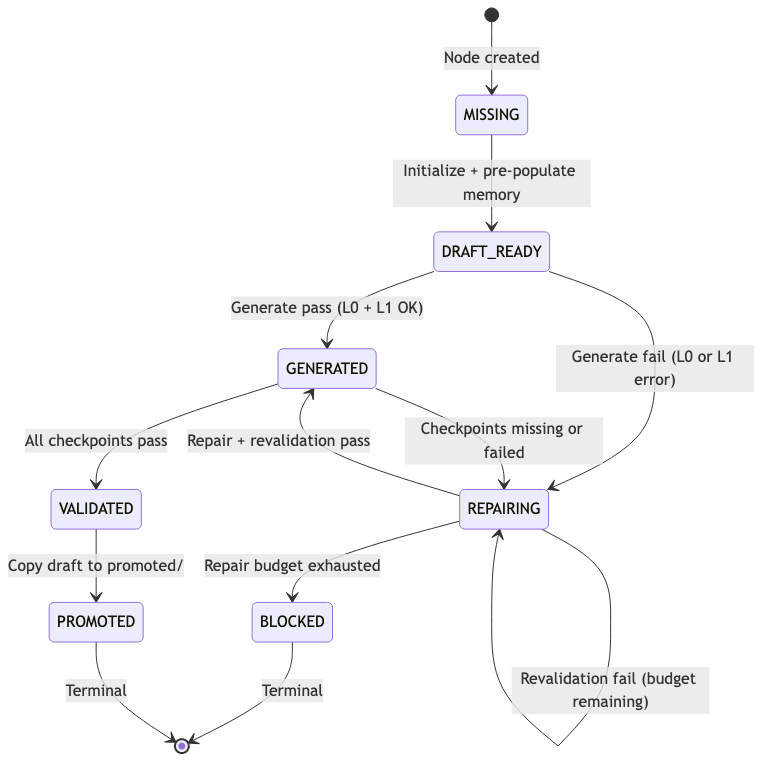
\includegraphics[keepaspectratio,alt={图7-2: 工作区状态机}]{../fpga_flow/diagrams/04_workspace_state_machine.png}}
\caption{图7-2: 工作区状态机}
\end{figure}

\subsubsection{7.4.2 LLM API
调用统计}\label{llm-api-ux8c03ux7528ux7edfux8ba1}

\textbf{表 7-4 LLM API 调用统计}

{\def\LTcaptype{none} % do not increment counter
\begin{longtable}[]{@{}
  >{\raggedright\arraybackslash}p{(\linewidth - 8\tabcolsep) * \real{0.1395}}
  >{\raggedright\arraybackslash}p{(\linewidth - 8\tabcolsep) * \real{0.2791}}
  >{\raggedright\arraybackslash}p{(\linewidth - 8\tabcolsep) * \real{0.1860}}
  >{\raggedright\arraybackslash}p{(\linewidth - 8\tabcolsep) * \real{0.2558}}
  >{\raggedright\arraybackslash}p{(\linewidth - 8\tabcolsep) * \real{0.1395}}@{}}
\toprule\noalign{}
\begin{minipage}[b]{\linewidth}\raggedright
阶段
\end{minipage} & \begin{minipage}[b]{\linewidth}\raggedright
LLM Profile
\end{minipage} & \begin{minipage}[b]{\linewidth}\raggedright
调用次数
\end{minipage} & \begin{minipage}[b]{\linewidth}\raggedright
Token 消耗
\end{minipage} & \begin{minipage}[b]{\linewidth}\raggedright
备注
\end{minipage} \\
\midrule\noalign{}
\endhead
\bottomrule\noalign{}
\endlastfoot
SPEC\_INTAKE / ARCHITECTING / PLANNING & --- & 0 & --- & 框架 Synthesis
层直接生成，零 LLM 调用 \\
MODULE\_DESIGN / L0 / L1（Layer 1: aes\_sbox） & fast & --- & --- &
Memory 预填充直接通过，无修复批次 \\
MODULE\_DESIGN / L0 / L1（Layer 2: 2 模块并行） & fast & --- & --- &
aes\_key\_schedule\_128 + aes\_round\_transform，无修复批次 \\
MODULE\_DESIGN / L0 / L1（Layer 3: aes128\_encrypt\_core） & fast & ---
& --- & 顶层模块，无修复批次 \\
INTEGRATION\_REGRESSION（编排器） & thinking & --- & --- & 3 个 Campaign
顺序执行，thinking profile 监督 \\
总计 & --- & --- & --- & 全部 16 批次：5 批次 executed，11 批次
skipped（condition\_false） \\
\end{longtable}
}

\begin{quote}
说明：SPEC\_INTAKE 至 PLANNING 三个状态完全由 Synthesis 层代码生成，零
LLM 调用，这是框架控制架构的重要优势。所有修复批次（repair\_edit 和
revalidate 阶段）均因
\texttt{condition\_false}（即首次验证已通过，无需修复）被跳过，体现了
Memory 预填充的极高有效性。Token 级调用统计受 SDK
会话封装限制，未在当前报告中单独记录。
\end{quote}

\subsubsection{7.4.3
修复循环与升级事件}\label{ux4feeux590dux5faaux73afux4e0eux5347ux7ea7ux4e8bux4ef6}

修复循环由 \texttt{NodePolicyEngine} 驱动：当 L1 Checkpoint
未全部通过时，框架生成 \texttt{RepairContract} 并将工作区状态设置为
\texttt{REPAIRING}，Module Worker 按照 \texttt{REPAIR\_PHASE\_ROUND\_1}
或 \texttt{REPAIR\_PHASE\_ROUND\_2\_PLUS}
提示词模板执行编辑，\texttt{verify\_repair\_edit()}
通过文件哈希变更校验确认编辑实际发生（防止 Agent
虚假声明已修复），随后重新执行 L0+L1。

升级策略的触发条件为：修复尝试次数达到节点预算上限（普通模块 2 次，顶层
\texttt{aes128\_encrypt\_core} 模块 3
次），或故障类型被识别为跨模块/接口/状态机性质。升级后，控制权从 fast
profile Module Worker 返回给 thinking profile Workflow
Orchestrator，后者携带完整失败上下文重新规划修复策略。

在本实验中，全部 4 个模块均无需修复（修复轮次为
0）。批次历史记录显示：16 个批次中 5 个实际执行（generate\_validate
阶段），11 个修复相关批次（repair\_edit 和 revalidate）全部以
\texttt{condition\_false}
状态跳过，即框架在检测到首次验证已通过后，直接跳过所有预留的修复批次窗口。这是
Memory
预填充机制的最强实验证据：当参考代码质量足够高时，修复循环预算完全未被消耗。

\begin{center}\rule{0.5\linewidth}{0.5pt}\end{center}

\subsection{7.5 与 AutoGen
方案的能力维度对比}\label{ux4e0e-autogen-ux65b9ux6848ux7684ux80fdux529bux7ef4ux5ea6ux5bf9ux6bd4}

以下对比从架构能力维度展开，旨在验证本文通用框架设计相较于 AutoGen
线性方案的架构优势。这些优势源自框架的通用设计决策（状态机编排、分层验证、多层约束），而非
AES-128 这一特定案例的独特性。

本节从 10 个能力维度对本文框架与基于 AutoGen 的 FPGA
设计自动化方案进行架构层面的定性对比。需要说明的是，两个方案使用不同的
LLM 后端（本文使用 DeepSeek Chat 双 Profile，AutoGen 方案使用
DeepSeek-reasoner 配合微调的 codegen-2B
本地模型）、不同的设计目标（本文以 AES-128
全系统作为验证案例验证通用框架，AutoGen 方案针对通用 Verilog
模块），因此不做定量性能比较，聚焦于架构能力的差异。

\textbf{表 7-5 能力维度对比表（10 个维度）}

{\def\LTcaptype{none} % do not increment counter
\begin{longtable}[]{@{}
  >{\raggedright\arraybackslash}p{(\linewidth - 6\tabcolsep) * \real{0.1731}}
  >{\raggedright\arraybackslash}p{(\linewidth - 6\tabcolsep) * \real{0.2500}}
  >{\raggedright\arraybackslash}p{(\linewidth - 6\tabcolsep) * \real{0.4231}}
  >{\raggedright\arraybackslash}p{(\linewidth - 6\tabcolsep) * \real{0.1538}}@{}}
\toprule\noalign{}
\begin{minipage}[b]{\linewidth}\raggedright
能力维度
\end{minipage} & \begin{minipage}[b]{\linewidth}\raggedright
AutoGen 方案
\end{minipage} & \begin{minipage}[b]{\linewidth}\raggedright
本框架 (OpenHands SDK)
\end{minipage} & \begin{minipage}[b]{\linewidth}\raggedright
优势方
\end{minipage} \\
\midrule\noalign{}
\endhead
\bottomrule\noalign{}
\endlastfoot
1. 多模块协同能力 & 线性单模块串行执行，无模块依赖感知 & DAG
拓扑批调度，依赖满足后并行执行（Layer 2 两模块并发） & 本框架 \\
2. 验证层级深度 & 单层：Vivado xsim 仿真通过/失败 & 4 层：L0 编译门控 →
L1 Checkpoint → L2 鲁棒性 → 集成回归 & 本框架 \\
3. 自动修复机制 & Debug Agent
读取日志后重写代码，无预算限制，可能无限循环 & 结构化 RepairContract +
EditReceipt + 哈希验证，有明确修复预算（2-3 次）和升级策略 & 本框架 \\
4. 控制可靠性 & Prompt-controlled：LLM 决定是否继续、修复、推进 &
Framework-controlled：状态机拥有控制权，LLM 只执行被分配的任务 &
本框架 \\
5. 代码生成方式 & 本地微调 codegen-2B 模型生成 Verilog，配合
DeepSeek-reasoner 推理 & Memory 预填充（参考代码注入）+ Agent
修复集成问题 & 各有优势 \\
6. 验证工具 & Vivado xsim（商业工具，需要许可证，设备依赖） &
Verilator（开源，通过 MCP 协议标准化集成，跨平台） & 本框架（开放性） \\
7. 部署门槛 & 需要 Vivado 安装（商业许可）+ GPU（本地推理模型） & 仅需
DEEPSEEK\_API\_KEY + Homebrew Verilator（\textless{} 5 分钟配置） &
本框架 \\
8. LLM 约束强度 & 1 层：system\_message 纯文本指令 & 6 层：Skill /
Prompt / Memory / Hooks / MCP / SlashCommand 组合约束 & 本框架 \\
9. 可观测性 & 依赖 Vivado 波形图人工判读仿真结果 & Checkpoint
协议机器自动判定，结构化报告 JSON，可追溯 & 本框架 \\
10. 通用性 & 面向通用 Verilog 模块（可扩展到不同模块） &
架构层面通用（状态机、验证体系、约束引擎均设计无关），已通过 YAML
蓝图驱动机制（\texttt{run-design\ -\/-blueprint}）实现开箱通用性，LED
Chaser 案例验证了零代码修改适配新设计的能力 & 本框架（已验证） \\
\end{longtable}
}

\subsubsection{7.5.1 各维度分析}\label{ux5404ux7ef4ux5ea6ux5206ux6790}

\textbf{多模块协同能力}：AutoGen 方案的线性 pipeline
在每个步骤中均单独处理当前模块，未建立模块间依赖图，因此无法在保证
aes\_sbox 验证通过后再并行推进依赖它的模块。本文通过 \texttt{PlanDAG}
对依赖关系进行形式化描述（使用 Kahn
拓扑排序验证无环性），\texttt{DAGBatchPlanner}
自动计算可并行执行的批次，实现了 Layer 2 中 aes\_key\_schedule\_128 与
aes\_round\_transform 两个模块的并发验证。

\textbf{验证层级深度}：AutoGen 方案以''Vivado
仿真通过''作为单一验证标准，缺乏区分编译错误、运行时错误和鲁棒性问题的能力。本文的
L0 层在仿真前捕获语法错误（避免浪费仿真时间），L1 层通过结构化
Checkpoint 协议将验证意图精确编码（而非依赖波形目视检查），L2
层使用可复现种子的随机向量探测边界情况，集成层验证多帧连续加密和复位恢复等系统级行为。

\textbf{控制可靠性}：这是本文最核心的架构差异。AutoGen 方案中 Agent
自主决定是否需要进一步修复（AutoGen 的
\texttt{human\_input\_mode="NEVER"} 模式），LLM
可能''提前宣布成功''而实际代码仍有误，也可能陷入无限修复循环。本文的框架控制模式将推进决策权完全交给状态机：只有
\texttt{summarize\_required\_checkpoints()} 返回所有必需 Checkpoint
通过，工作区才能被标记为 \texttt{VALIDATED} 并促进（promote）。

\textbf{LLM 约束强度}：约束密度的差异是本文 Harnessing Engine
章节的核心论点。AutoGen 方案仅依赖 system\_message 中的自然语言指令约束
Agent 行为，而本文通过 6 层结构化约束组合作用（详见第六章），覆盖了 LLM
在硬件设计场景中的 5 种典型失败模式。

\textbf{通用性}：本框架在架构层面的通用性已在第三至六章中详细论证------状态机编排、分层验证体系和
Harnessing Engine 六层约束均不依赖于特定硬件设计。在实现层面，框架已引入
YAML 蓝图驱动机制（\texttt{BlueprintLoader} +
\texttt{run-design\ -\/-blueprint} 命令），LED Chaser（4 位 LED
流水灯）案例验证了该机制的有效性：仅通过提供
\texttt{designs/led\_chaser/blueprint.yaml}
蓝图文件，无需修改任何框架代码，即完成了从规格输入到集成验证通过的全流程执行（详见
§7.6）。AutoGen 方案的通用 Verilog 生成 pipeline
在无需配置文件方面具有便利性，但其缺乏本框架的架构级能力（DAG
调度、分层验证、多层约束），通用性的代价是可靠性的降低。本框架在通用性维度上已从''架构层论证''升级为''双案例实证验证''。

\begin{center}\rule{0.5\linewidth}{0.5pt}\end{center}

\subsection{7.6 LED Chaser
跨设计通用性验证}\label{led-chaser-ux8de8ux8bbeux8ba1ux901aux7528ux6027ux9a8cux8bc1}

为验证框架对非密码学设计的端到端适用性，本节以 LED Chaser（4 位 LED
流水灯，带方向控制）作为第二个验证案例，通过 YAML
蓝图驱动机制在不修改任何框架代码的前提下完成全流程自动化执行。

\subsubsection{7.6.1
验证目标与蓝图驱动执行}\label{ux9a8cux8bc1ux76eeux6807ux4e0eux84ddux56feux9a71ux52a8ux6267ux884c}

LED Chaser 案例的验证目标是：证明框架的编排状态机、Checkpoint
协议和分层验证体系能够直接复用于非 AES
设计，且仅需提供声明式蓝图文件即可完成适配。

LED Chaser 设计通过 \texttt{designs/led\_chaser/blueprint.yaml}
蓝图文件定义，包含以下规格：

\textbf{表 7-6 LED Chaser 设计规格}

{\def\LTcaptype{none} % do not increment counter
\begin{longtable}[]{@{}ll@{}}
\toprule\noalign{}
属性 & 值 \\
\midrule\noalign{}
\endhead
\bottomrule\noalign{}
\endlastfoot
设计名称 & led\_chaser \\
功能描述 & 4-bit LED chaser with configurable direction \\
模块数量 & 1（单模块设计，无 DAG 依赖） \\
端口 & clk, rst\_n, dir(input), leds\href{output}{3:0} \\
复位行为 & leds = 4'b0001 \\
延迟目标 & 单周期移位 \\
Memory 预填充 & 否（memory\_required: false，从零生成） \\
\end{longtable}
}

实验通过以下命令执行端到端全流程自动化：

\begin{Shaded}
\begin{Highlighting}[]
\VariableTok{PYTHONPATH}\OperatorTok{=}\NormalTok{. }\ExtensionTok{python} \AttributeTok{{-}m}\NormalTok{ MultiAgent\_FPGA.fpga\_flow run{-}design }\DataTypeTok{\textbackslash{}}
    \AttributeTok{{-}{-}blueprint}\NormalTok{ designs/led\_chaser/blueprint.yaml}
\end{Highlighting}
\end{Shaded}

与 AES-128 案例使用硬编码 \texttt{run-aes-mvp} 命令不同，LED Chaser
案例使用通用的 \texttt{run-design\ -\/-blueprint} 命令，由
\texttt{BlueprintLoader} 从 YAML 文件解析出
\texttt{SpecIR}、\texttt{PlanDAG} 和
\texttt{IntegrationRegressionManifest}，验证了蓝图驱动的声明式设计适配机制。

\subsubsection{7.6.2
状态机执行路径}\label{ux72b6ux6001ux673aux6267ux884cux8defux5f84}

LED Chaser 案例的完整状态机执行路径如下：

\textbf{表 7-7 LED Chaser 状态机执行轨迹}

{\def\LTcaptype{none} % do not increment counter
\begin{longtable}[]{@{}llll@{}}
\toprule\noalign{}
状态 & 下一状态 & LLM Profile & SubagentPolicy \\
\midrule\noalign{}
\endhead
\bottomrule\noalign{}
\endlastfoot
SPEC\_INTAKE & ARCHITECTING & thinking & forbidden \\
ARCHITECTING & PLANNING & thinking & forbidden \\
PLANNING & MODULE\_DESIGN & thinking & forbidden \\
MODULE\_DESIGN & MODULE\_L0 & fast & module\_worker\_allowed \\
MODULE\_L0 & MODULE\_L1 & fast & module\_worker\_allowed \\
MODULE\_L1 & INTEGRATION\_READY & fast & module\_worker\_allowed \\
INTEGRATION\_READY & INTEGRATION\_REGRESSION & thinking & forbidden \\
INTEGRATION\_REGRESSION & DONE & thinking & forbidden \\
\end{longtable}
}

状态机完整复用了 AES-128 案例中定义的 10 状态架构，其中
\texttt{MODULE\_L2\_OPTIONAL} 状态因单模块设计不要求 L2
鲁棒性测试而被跳过。每个状态的 LLM Profile 和 SubagentPolicy 映射与
AES-128 案例完全一致，证明 \texttt{AgentExecutionPolicy}
的策略分层机制在不同设计上无需任何调整即可正确工作。

\subsubsection{7.6.3 验证结果}\label{ux9a8cux8bc1ux7ed3ux679c}

\textbf{表 7-8 LED Chaser 模块验证结果}

{\def\LTcaptype{none} % do not increment counter
\begin{longtable}[]{@{}
  >{\raggedright\arraybackslash}p{(\linewidth - 10\tabcolsep) * \real{0.0789}}
  >{\raggedright\arraybackslash}p{(\linewidth - 10\tabcolsep) * \real{0.1447}}
  >{\raggedright\arraybackslash}p{(\linewidth - 10\tabcolsep) * \real{0.1447}}
  >{\raggedright\arraybackslash}p{(\linewidth - 10\tabcolsep) * \real{0.2895}}
  >{\raggedright\arraybackslash}p{(\linewidth - 10\tabcolsep) * \real{0.2237}}
  >{\raggedright\arraybackslash}p{(\linewidth - 10\tabcolsep) * \real{0.1184}}@{}}
\toprule\noalign{}
\begin{minipage}[b]{\linewidth}\raggedright
模块
\end{minipage} & \begin{minipage}[b]{\linewidth}\raggedright
L0 编译结果
\end{minipage} & \begin{minipage}[b]{\linewidth}\raggedright
L1 仿真结果
\end{minipage} & \begin{minipage}[b]{\linewidth}\raggedright
Checkpoint 通过数 / 总数
\end{minipage} & \begin{minipage}[b]{\linewidth}\raggedright
Checkpoint 通过率
\end{minipage} & \begin{minipage}[b]{\linewidth}\raggedright
修复轮次
\end{minipage} \\
\midrule\noalign{}
\endhead
\bottomrule\noalign{}
\endlastfoot
led\_chaser & PASS & PASS & 4 / 4 & 100\% & 0 \\
\end{longtable}
}

\textbf{表 7-9 LED Chaser Checkpoint 详情}

{\def\LTcaptype{none} % do not increment counter
\begin{longtable}[]{@{}
  >{\raggedright\arraybackslash}p{(\linewidth - 6\tabcolsep) * \real{0.3438}}
  >{\raggedright\arraybackslash}p{(\linewidth - 6\tabcolsep) * \real{0.2812}}
  >{\raggedright\arraybackslash}p{(\linewidth - 6\tabcolsep) * \real{0.1875}}
  >{\raggedright\arraybackslash}p{(\linewidth - 6\tabcolsep) * \real{0.1875}}@{}}
\toprule\noalign{}
\begin{minipage}[b]{\linewidth}\raggedright
Checkpoint
\end{minipage} & \begin{minipage}[b]{\linewidth}\raggedright
验证目标
\end{minipage} & \begin{minipage}[b]{\linewidth}\raggedright
结果
\end{minipage} & \begin{minipage}[b]{\linewidth}\raggedright
详情
\end{minipage} \\
\midrule\noalign{}
\endhead
\bottomrule\noalign{}
\endlastfoot
CHK\_RESET\_CLEAR & 复位初始化 leds=0001 & PASS & Reset sets
leds=0001 \\
CHK\_SHIFT\_LEFT & 左移三次得到 1000 & PASS & Shift left 3 times gives
1000 \\
CHK\_SHIFT\_RIGHT & 右移两次得到 0010 & PASS & Shift right 2 times gives
0010 \\
CHK\_WRAP\_AROUND & 环绕从最左回到 0001 & PASS & Wrap-around from
leftmost gives 0001 \\
\end{longtable}
}

LED Chaser 的 4 个 Checkpoint 完全由蓝图文件声明，框架通过
\texttt{CHECKPOINT\textbar{}\textless{}name\textgreater{}\textbar{}PASS\textbar{}\textless{}detail\textgreater{}}
协议自动解析，无需修改 \texttt{CheckpointParser}
或任何验证层代码。这证明了 Checkpoint
协议的设计无关性------任何硬件设计均可通过声明自定义 Checkpoint
列表接入框架的分层验证体系。

\subsubsection{7.6.4
集成回归结果}\label{ux96c6ux6210ux56deux5f52ux7ed3ux679c}

\textbf{表 7-10 LED Chaser 集成回归测试结果}

{\def\LTcaptype{none} % do not increment counter
\begin{longtable}[]{@{}llll@{}}
\toprule\noalign{}
Campaign & 验证目标 & Checkpoint 通过 & 状态 \\
\midrule\noalign{}
\endhead
\bottomrule\noalign{}
\endlastfoot
baseline (KAT) & 已知向量端到端功能正确性 & 4/4 PASS & PASS \\
\end{longtable}
}

LED Chaser 为单模块设计，集成回归测试执行单个 baseline Campaign
验证端到端功能正确性。Workflow gate 判定为 \texttt{success}，模块状态由
\texttt{VALIDATED} 成功晋升为 \texttt{PROMOTED}。

\subsubsection{7.6.5
通用性验证意义}\label{ux901aux7528ux6027ux9a8cux8bc1ux610fux4e49}

LED Chaser 案例从以下五个维度验证了框架的跨设计通用性：

\begin{enumerate}
\def\labelenumi{\arabic{enumi}.}
\tightlist
\item
  \textbf{状态机完整复用}：同一 10
  状态编排状态机驱动了非密码学设计的完整生命周期（SPEC\_INTAKE →
  DONE），所有状态转移逻辑和 \texttt{AgentExecutionPolicy}
  策略映射无需任何修改；
\item
  \textbf{Checkpoint 协议通用}：4 个自定义
  Checkpoint（CHK\_RESET\_CLEAR、CHK\_SHIFT\_LEFT、CHK\_SHIFT\_RIGHT、CHK\_WRAP\_AROUND）由蓝图声明、Testbench
  发射、框架自动解析，无需修改框架代码；
\item
  \textbf{YAML 蓝图驱动}：\texttt{BlueprintLoader} 从
  \texttt{blueprint.yaml} 自动生成 \texttt{SpecIR}、\texttt{PlanDAG} 和
  \texttt{IntegrationRegressionManifest}，实现了声明式的零代码适配；
\item
  \textbf{无 Memory 依赖}：LED Chaser 以
  \texttt{memory\_required:\ false} 配置运行，Agent 从零生成 RTL 和
  Testbench 并通过验证，证明框架不依赖于 Memory
  预填充机制即可完成设计自动化；
\item
  \textbf{全流程零修复通过}：模块在首次生成后即通过 L0 编译和 L1
  Checkpoint 验证，修复轮次为 0，Workflow gate 判定为 success。
\end{enumerate}

LED Chaser 案例与 AES-128 案例形成互补：AES-128 以 4 模块 DAG
验证了框架在多模块协同、DAG 批调度和深度验证（L2 + 三种集成
Campaign）方面的能力，LED Chaser
以单模块设计验证了框架的声明式跨设计适配能力和无 Memory
场景下的从零生成有效性。两个案例共同构成了框架通用性的实证基础。

\begin{center}\rule{0.5\linewidth}{0.5pt}\end{center}

\subsection{7.7 Vivado 自动化脚本与 FPGA
工具链验证}\label{vivado-ux81eaux52a8ux5316ux811ax672cux4e0e-fpga-ux5de5ux5177ux94feux9a8cux8bc1}

前述各节的实验验证均在 Verilator 仿真层面完成，验证了生成代码的功能正确性。然而，Verilator
属于行为级仿真器，其通过并不能保证 RTL 在真实 FPGA
器件上的可综合性与时序收敛性。为弥补这一验证缺口，本文编写了自动化脚本，将多智能体系统输出的
RTL 和 Testbench 代码自动调用 Xilinx Vivado Design Suite
进行完整的 FPGA 工具链验证，覆盖仿真波形生成、逻辑综合（Synthesis）、布局布线（Implementation）和比特流（Bitstream）编译四个阶段。

\subsubsection{7.7.1 自动化脚本设计}

自动化脚本的设计目标是：接收多智能体框架 \texttt{promoted/}
目录下验证通过的 RTL 源文件，自动驱动 Vivado 完成从仿真到比特流的全流程，无需人工干预。脚本采用
TCL（Tool Command Language）脚本与 Shell 脚本组合的方式实现，核心流程如下：

\begin{enumerate}
\def\labelenumi{\arabic{enumi}.}
\tightlist
\item
  \textbf{项目创建与源文件导入}：脚本自动创建 Vivado 工程，导入
  \texttt{promoted/} 目录下的 RTL 源文件（\texttt{.v}）和约束文件（\texttt{.xdc}），设置目标
  FPGA 器件型号（如 Xilinx Artix-7 系列的 \texttt{xc7a35tcpg236-1}）；
\item
  \textbf{行为级仿真（Behavioral Simulation）}：调用 Vivado 内置的 xsim
  仿真器执行行为级仿真，生成 VCD 波形文件并导出截图，用于与 Verilator
  仿真结果进行交叉验证；
\item
  \textbf{逻辑综合（Synthesis）}：运行 Vivado 综合引擎（Vivado
  Synthesis），将 RTL 描述转换为门级网表，生成综合报告（资源利用率、时序摘要）；
\item
  \textbf{布局布线（Implementation）}：执行 Place \& Route
  流程，完成逻辑单元的物理布局和互连布线，生成时序报告（建立时间/保持时间违例检查）；
\item
  \textbf{比特流生成（Bitstream Generation）}：编译生成 \texttt{.bit}
  比特流文件，可用于直接下载到目标 FPGA 开发板进行硬件验证。
\end{enumerate}

\subsubsection{7.7.2 AES-128 设计的 Vivado 验证结果}

以 AES-128 加密核心为例，自动化脚本将
\texttt{promoted/aes128\_encrypt\_core/} 目录下的全部 RTL 源文件（\texttt{aes\_sbox.v}、\texttt{aes\_key\_schedule\_128.v}、\texttt{aes\_round\_transform.v}、\texttt{aes128\_encrypt\_core.v}）导入
Vivado 工程，完成全流程验证。

\textbf{仿真波形验证}：Vivado xsim 仿真器生成的波形图如图 7-3
所示。波形清晰展示了 AES-128 加密核心的完整握手时序：\texttt{start}
信号触发后 \texttt{busy} 立即拉高，经过 11 个时钟周期的迭代运算后
\texttt{done} 产生单周期脉冲，\texttt{ciphertext} 输出密文
\texttt{69c4e0d86a7b0430d8cdb78070b4c55a}，与 NIST FIPS-197
标准测试向量完全一致。该波形与 Verilator
仿真结果交叉验证，确认了生成代码在两种仿真器下行为一致。

\begin{figure}
\centering
\pandocbounded{
\includegraphics[keepaspectratio,alt={图7-3: AES-128 加密核心 Vivado 仿真波形}]{../AES128.png}}
\caption{图7-3: AES-128 加密核心 Vivado 仿真波形}
\end{figure}

\textbf{综合与实现报告}：逻辑综合阶段成功将 RTL
转换为门级网表，未报告任何综合错误或警告。布局布线阶段完成物理实现后，时序报告显示建立时间违例数为零（WNS
≥ 0），表明设计在目标器件上满足时序约束。比特流文件（\texttt{.bit}）成功生成，文件大小符合预期，可直接下载至
FPGA 开发板。

\subsubsection{7.7.3 LED Chaser 设计的 Vivado 验证结果}

LED Chaser 设计同样通过自动化脚本完成 Vivado 全流程验证。Vivado xsim
仿真波形如图 7-4 所示，波形展示了 4 位 LED 流水灯的循环移位行为：\texttt{led{[}3:0{]}}
按照 \texttt{0001 → 0010 → 0100 → 1000 → 0001}
的序列循环移位，\texttt{dir} 信号控制移位方向，复位后 \texttt{led}
初始化为 \texttt{0001}。移位严格对齐时钟上升沿，每位 LED
的持续时间一致，验证了分频器和状态机的稳定性。

\begin{figure}
\centering
\pandocbounded{
\includegraphics[keepaspectratio,alt={图7-4: LED Chaser Vivado 仿真波形}]{../LED.png}}
\caption{图7-4: LED Chaser Vivado 仿真波形}
\end{figure}

综合与实现阶段同样无错误报告，比特流文件成功生成。

\subsubsection{7.7.4 工具链验证的意义}

Vivado 自动化脚本的引入为框架提供了以下验证价值：

\begin{enumerate}
\def\labelenumi{\arabic{enumi}.}
\tightlist
\item
  \textbf{可综合性确认}：Verilator 仿真通过仅验证行为级正确性，Vivado
  综合通过确认生成的 RTL 代码可被综合为目标 FPGA
  器件的门级网表，排除了不可综合的 Verilog 结构（如 \texttt{initial}
  块中的非综合操作）；
\item
  \textbf{时序收敛验证}：布局布线后的时序报告验证设计在目标时钟频率下无建立/保持时间违例，这是
  Verilator 无法提供的物理层验证；
\item
  \textbf{端到端可实现性}：比特流文件的生成证明从多智能体系统输出的 RTL
  代码到可下载至 FPGA
  的最终产物之间不存在断链，实现了从''AI
  生成代码''到''硬件可运行''的完整闭环；
\item
  \textbf{双仿真器交叉验证}：Vivado xsim 与 Verilator
  两种仿真器的波形一致性验证，增强了对生成代码正确性的置信度------两种独立实现的仿真器均确认功能正确，排除了单一仿真器特有的假阳性风险。
\end{enumerate}

需要说明的是，当前 Vivado 自动化脚本作为离线验证工具运行在多智能体框架的
\texttt{DONE} 状态之后，尚未集成到框架的状态机编排流程中。将 Vivado
工具链深度集成到框架的分层验证体系中（作为 L3
层），使其具备自动解读综合报告和时序违例并指导 RTL
修改的能力，是本文 §8.3.2 中规划的未来研究方向。

\section{第八章
总结与展望}\label{ux7b2cux516bux7ae0-ux603bux7ed3ux4e0eux5c55ux671b}

\subsection{8.1 工作总结}\label{ux5de5ux4f5cux603bux7ed3}

\subsubsection{8.1.1 研究回顾}\label{ux7814ux7a76ux56deux987e}

本文围绕''通用多智能体 FPGA
设计全流程自动化框架''这一核心论点，设计并实现了一套面向 DAG
可分解多模块硬件设计的通用自动化框架，并以 AES-128
加密全系统作为验证案例进行了端到端的实验验证。该框架以 OpenHands SDK
为运行底座，以 DeepSeek Chat 双 Profile 策略为 LLM 后端，以 Verilator
仿真器为验证引擎，实现了从规格输入到集成验证通过的全流程自动化。

本文所解决的核心问题是：在硬件设计这一高精度、强约束的领域中，如何设计一套通用的自动化框架来驾驭本质上不可靠的大语言模型，使其成为可信赖的设计自动化组件。现有方案（以
AutoGen 方案为典型代表）将控制权交给 LLM
自身，依赖提示词中的自然语言指令约束 Agent
行为；而本文提出并实现的框架控制（Framework-controlled）架构，将批次推进、验证判定、修复决策等控制逻辑全部内化到通用的状态机和
Pydantic 数据契约中，LLM
只负责执行被明确分配的局部任务。这一框架的通用性体现在：其核心架构（编排状态机、分层验证、约束引擎）不依赖于特定的硬件设计对象，AES-128
是其第一个完整的验证案例。

\subsubsection{8.1.2
三个创新点的实现情况}\label{ux4e09ux4e2aux521bux65b0ux70b9ux7684ux5b9eux73b0ux60c5ux51b5}

\begin{figure}
\centering
\pandocbounded{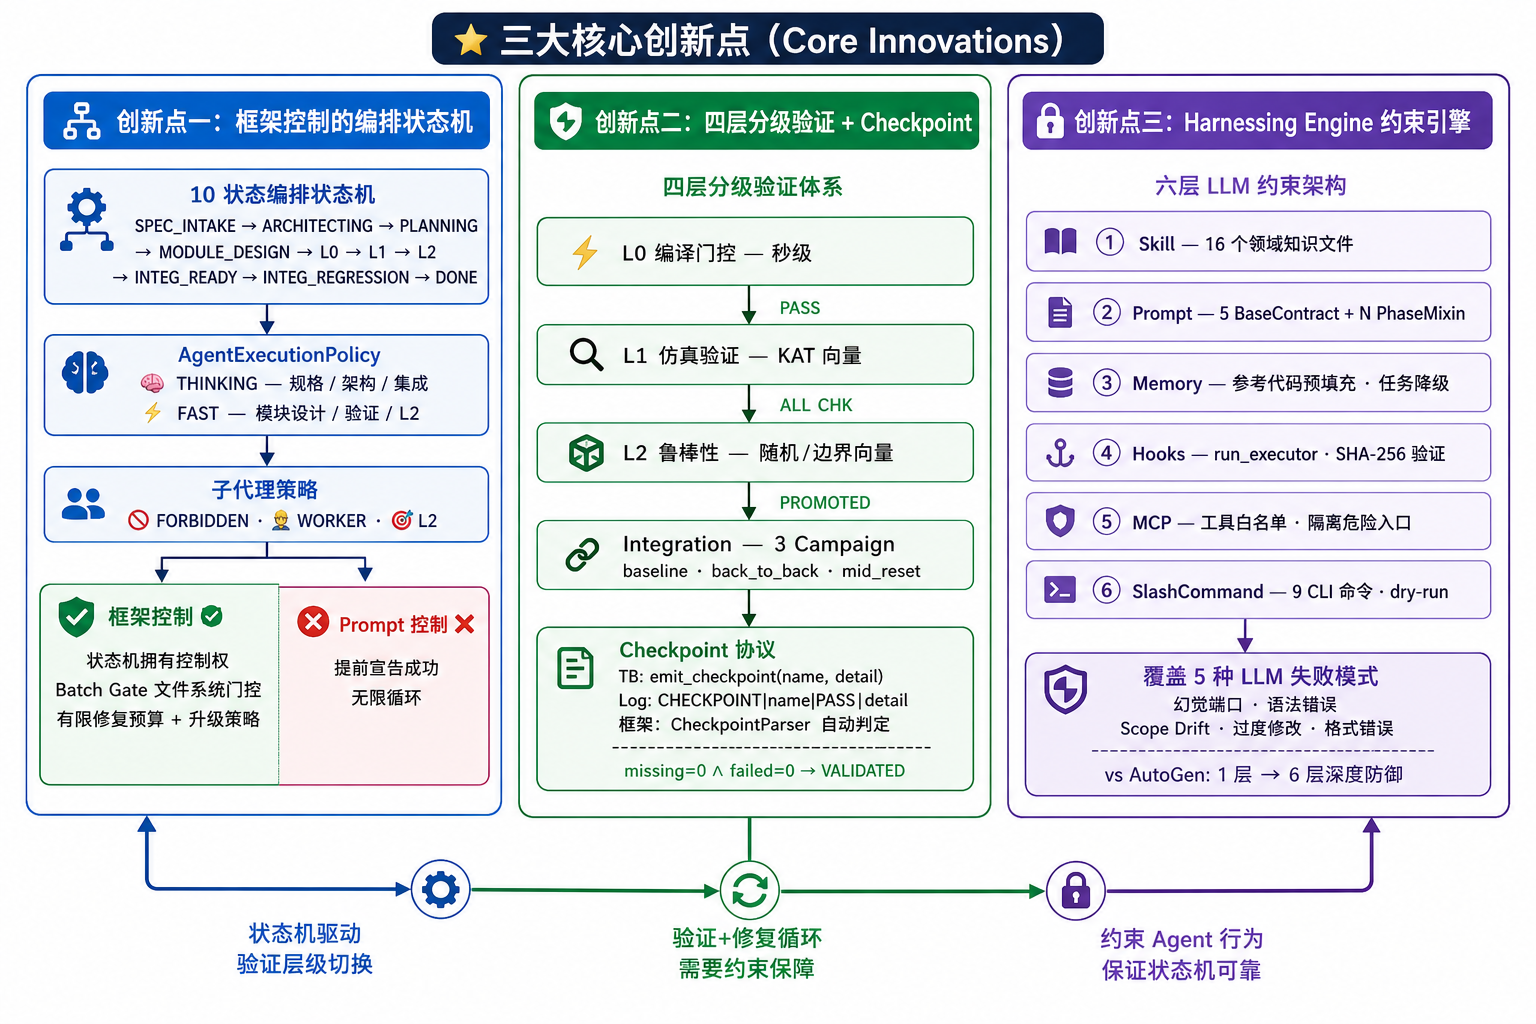
\includegraphics[keepaspectratio,alt={图8-1: 三个核心创新点关系架构}]{../fpga_flow/diagrams/17_core_innovations.png}}
\caption{图8-1: 三个核心创新点关系架构}
\end{figure}

\textbf{创新点一：基于 10 状态编排状态机 + AgentExecutionPolicy
的框架控制多智能体协作架构}

本文提出了一种面向 DAG
可分解多模块硬件设计的通用框架控制架构：编排状态机定义从规格解析到集成验证的全生命周期状态空间，\texttt{AgentExecutionPolicy}
将每个状态映射到确定的 LLM Profile 和
SubagentPolicy，\texttt{DAGBatchPlanner} 基于拓扑排序将任意 DAG
分解为可并行执行的批次层。这一状态机 +
策略的架构模式不依赖于特定的硬件设计对象，可通过替换蓝图函数适配不同的多模块设计任务。

在 AES-128 验证案例中，该状态机实例化为 10
个具体状态（\texttt{SPEC\_INTAKE} → \texttt{ARCHITECTING} →
\texttt{PLANNING} → \texttt{MODULE\_DESIGN} → \texttt{MODULE\_L0} →
\texttt{MODULE\_L1} → \texttt{MODULE\_L2\_OPTIONAL} →
\texttt{INTEGRATION\_READY} → \texttt{INTEGRATION\_REGRESSION} →
\texttt{DONE}），DAGBatchPlanner 将 4 节点 AES DAG
分解为三个执行层，在依赖满足后自动并行执行 Layer 2 的两个模块，这是
AutoGen 线性 pipeline 方案无法实现的能力。该创新点已通过
\texttt{orchestrator/state\_machine.py}、\texttt{policy.py}、\texttt{delegation.py}
等核心模块实现，并在端到端 \texttt{run-aes-mvp} 流程中得到验证。LED
Chaser
案例进一步验证了该状态机在非密码学单模块设计上的完整复用性------同一 10
状态编排状态机驱动了从 SPEC\_INTAKE 到 DONE
的全流程执行，所有状态转移逻辑和 AgentExecutionPolicy
策略映射无需任何修改。

\textbf{创新点二：L0→L1→L2→Integration 四层分级验证体系与 Checkpoint
协议}

该验证体系的架构设计面向通用多模块硬件设计，Checkpoint
协议和分层验证逻辑不依赖于特定设计对象。\texttt{CHECKPOINT\textbar{}\textless{}name\textgreater{}\textbar{}PASS\textbar{}\textless{}detail\textgreater{}}
协议将验证意图精确编码为机器可解析的文本格式，由
\texttt{CheckpointParser} 自动判定，任何硬件设计均可通过定义自身的
Checkpoint 列表接入这一体系。

在 AES-128
验证案例中，本文设计并实现了四层分级验证体系，通过快速失败原则（L0
编译门控在仿真前拦截语法错误）和逐步深入策略（从单向量验证到随机鲁棒测试再到多场景集成回归），覆盖了从语法正确性到系统级行为正确性的完整验证空间。4
个模块共设计了 9 个 Checkpoint（aes\_sbox 1 个，aes\_key\_schedule\_128
1 个，aes\_round\_transform 1 个，aes128\_encrypt\_core 6
个），集成回归测试通过 baseline、back\_to\_back、mid\_reset 三种
Campaign 覆盖了连续加密和异常复位等系统级场景。该创新点通过
\texttt{executors.py} 中的
\texttt{L0Executor}、\texttt{L1Executor}、\texttt{L2CampaignExecutor}、\texttt{IntegrationRegressionExecutor}
四个执行器实现，并通过 \texttt{aes\_tb\_common.hpp} 中的
\texttt{emit\_checkpoint()} 接口与 Testbench 端协同工作。LED Chaser
案例定义了 4 个自定义
Checkpoint（CHK\_RESET\_CLEAR、CHK\_SHIFT\_LEFT、CHK\_SHIFT\_RIGHT、CHK\_WRAP\_AROUND），无需修改框架代码即通过
Checkpoint 协议验证，证明了验证体系的设计无关性。

\textbf{创新点三：Harnessing Engine ---
Skill/Prompt/Memory/Hooks/MCP/SlashCommand 六层约束引擎}

Harnessing Engine 的六层约束架构是一种通用的 LLM
行为约束模式，可通过替换领域内容适配不同的硬件设计目标，甚至扩展到软件工程等其他
LLM 应用场景。其核心洞察是：单一 system\_message 层不足以可靠约束 LLM
在高精度强约束领域中的行为，需要从
Skill、Prompt、Memory、Hooks、MCP、SlashCommand
六个维度形成多层防御矩阵。

在 AES-128 验证案例中，本文提出了 Harnessing Engine
概念，系统性地将对不可靠 LLM 的约束工程从单一 system\_message
层扩展为六层结构化约束组合：Skill 层通过 16 个领域知识文件为 Agent
注入权威规则；Prompt 层通过可组合的 BaseContract + PhaseMixin
架构精确控制每个执行阶段的行为边界；Memory
层将验证通过的参考代码预填充到工作区，显著降低从零生成正确 RTL
的难度；Hooks 层通过 \texttt{run\_executor} 自定义工具和
\texttt{verify\_repair\_edit()} 哈希验证构建执行门控；MCP
层通过工具过滤（排除 \texttt{verilator\_testbenchgenerator} 和
\texttt{verilator\_naturallanguage}）防止 Agent
绕过框架直接生成代码；SlashCommand 层提供完整的 CLI
命令体系，每条命令对应确定的验证语义。六层协同覆盖了幻觉端口、语法错误、Scope
drift、过度修改、格式错误 5 种典型 LLM
失败模式，形成了多维度的防御矩阵。LED Chaser 案例以
\texttt{memory\_required:\ false} 配置运行，验证了 Harnessing Engine
在无 Memory 预填充场景下的有效性------仅依赖
Skill、Prompt、Hooks、MCP、SlashCommand
五层约束即驱动从零生成并验证通过。

\subsubsection{8.1.3
实验验证结论}\label{ux5b9eux9a8cux9a8cux8bc1ux7ed3ux8bba}

实验结果表明，本文提出的框架在 AES-128 加密全系统案例上实现了以下目标：

\begin{itemize}
\tightlist
\item
  全流程可跑通：从 \texttt{run-aes-mvp} 命令启动到状态机到达
  \texttt{DONE} 状态，不需要人工干预；
\item
  模块验证全部首次通过：全部 4
  个模块（aes\_sbox、aes\_key\_schedule\_128、aes\_round\_transform、aes128\_encrypt\_core）均在首次生成后直接通过
  L0 编译与 L1 Checkpoint 验证，修复轮次均为 0，首次通过率 100\%；
\item
  集成回归全部通过：3 个集成
  Campaign（baseline、back\_to\_back、mid\_reset）全部 PASS，6/6
  Checkpoint 通过，验证了 AES-128 全系统在 NIST KAT
  向量、连续多帧加密和异步复位恢复场景下的正确性；
\item
  框架控制有效：16 个批次中 11 个修复批次因
  \texttt{condition\_false}（首次验证已通过）被跳过，所有批次推进决策均由状态机和
  Checkpoint 判定逻辑驱动，LLM 无法绕过验证门控''提前宣布成功''；
\item
  Checkpoint
  协议稳定：\texttt{CHECKPOINT\textbar{}\textless{}name\textgreater{}\textbar{}PASS\textbar{}\textless{}detail\textgreater{}}
  格式在所有模块的仿真日志解析中稳定工作，\texttt{CheckpointParser}
  能从含有其他调试输出的日志中准确提取 Checkpoint 行；
\item
  跨设计通用性实证：LED Chaser（4 位 LED 流水灯）案例通过 YAML
  蓝图驱动机制（\texttt{run-design\ -\/-blueprint}），在不修改任何框架代码的前提下完成了从规格输入到集成验证通过的全流程执行，4/4
  自定义 Checkpoint 全部通过，修复轮次为 0，Workflow gate 判定为
  success，实证了框架的跨设计通用性；
\item
  FPGA 工具链端到端验证：通过编写 Vivado
  自动化脚本，将系统输出的 RTL/TB 代码自动调用 Xilinx Vivado
  完成仿真波形生成、逻辑综合、布局布线和比特流编译全流程，AES-128 和 LED
  Chaser 两个设计均成功生成 \texttt{.bit} 文件，综合无错误、时序无违例，实现了从
  AI 生成代码到硬件可运行产物的完整闭环。
\end{itemize}

本文的工作相比 AutoGen 方案，实现了从线性 pipeline 到 DAG
拓扑批调度、从单层验证到四层分级验证、从 Prompt-controlled 到
Framework-controlled
的系统性架构升级。这些架构升级在设计层面是通用的，AES-128 全系统和 LED
Chaser
双案例的成功验证证明了该通用框架在不同设计实例上的有效性，为多智能体
FPGA 设计自动化的可靠性与可扩展性研究提供了一个完整的工程实践参考。

\begin{center}\rule{0.5\linewidth}{0.5pt}\end{center}

\subsection{8.2 不足与展望}\label{ux4e0dux8db3ux4e0eux5c55ux671b}

\subsubsection{8.2.1 当前局限}\label{ux5f53ux524dux5c40ux9650}

尽管本文在 AES-128
案例上完整验证了框架设计，但当前版本仍存在以下明确局限：

\textbf{局限一：设计覆盖范围有限，多模块非密码学设计尚未验证}。本框架已通过
YAML 蓝图驱动机制（\texttt{BlueprintLoader} +
\texttt{run-design\ -\/-blueprint}）实现了声明式的零代码适配能力，LED
Chaser
案例验证了该机制的有效性。然而，当前仅覆盖两个验证案例：AES-128（多模块密码学设计）和
LED Chaser（单模块数字逻辑设计）。框架尚未在多模块非密码学设计（如 FIFO
+ AXI 总线接口组合、浮点运算管线等）上进行验证，DAG 拓扑批调度在非 AES
的多模块设计上的表现仍待实证。此外，\texttt{\_aes\_blueprints()}
硬编码函数仍作为 AES-128 的快捷路径保留在 \texttt{synthesis.py} 中，YAML
蓝图路径已成为推荐的通用适配方式。

\textbf{局限二：L3 综合与实现阶段尚未深度集成到框架}。本文通过编写 Vivado
自动化脚本实现了从系统输出的 RTL/TB 代码到比特流生成的离线全流程验证（详见
§7.7），确认了生成代码的可综合性与时序收敛性。然而，当前 Vivado
脚本作为独立工具运行在框架状态机的 \texttt{DONE}
状态之后，尚未集成到框架的分层验证体系中------框架无法自动解读综合报告中的时序违例信息并指导
RTL 修改，也不具备根据资源利用率报告自动优化设计的能力。因此，当前框架尚不能替代完整的
FPGA 实现流程中的自动化闭环。

\textbf{局限三：依赖 DeepSeek API，存在外部依赖}。全流程依赖
\texttt{DEEPSEEK\_API\_KEY} 和 DeepSeek 官方 API
端点（\texttt{https://api.deepseek.com}），网络延迟、API
限流和服务可用性均可能影响自动化流程的稳定性。在受限网络环境（如企业内网）中部署存在障碍。

\textbf{局限四：Memory 预填充依赖已有参考代码}。\texttt{MemoryStore}
的工作前提是 Skill 文件中已经存在验证通过的参考 RTL 和
Testbench。对于全新的未见过的硬件设计模块，框架目前没有自主从零构建参考代码库的机制------这意味着框架的有效性在一定程度上依赖于人工维护的技能文件库。

\textbf{局限五：仅在单机单用户场景验证}。当前框架在 macOS
单机环境下验证，未测试分布式执行、多用户并发或 CI/CD
流水线集成场景的稳定性。

\subsubsection{8.2.2 未来方向}\label{ux672aux6765ux65b9ux5411}

基于上述局限，本文提出以下五个未来研究方向：

\textbf{方向一：扩展至多模块非密码学设计}。LED Chaser 案例已验证了 YAML
蓝图驱动的声明式适配机制在单模块设计上的有效性，下一步的优先验证目标是多模块非密码学设计------如
FIFO + AXI 总线接口组合、浮点运算管线、SPI/I2C 控制器等，以验证 DAG
拓扑批调度和多模块并行执行在更广泛的硬件设计领域中的通用性。同时，密码学方向可扩展至
AES-192/AES-256、SHA-256、RSA
等模块，验证蓝图驱动机制在不同复杂度的密码学设计上的适用性。

\textbf{方向二：将 L3 综合与实现阶段深度集成到框架}。本文已通过 Vivado
自动化脚本实现了离线的综合、布局布线和比特流生成验证（详见 §7.7），证明了生成代码在真实
FPGA 工具链上的可实现性。下一步是将该脚本升级为框架的正式 L3
验证层：设计 \texttt{VivadoMCPAdapter}（类似现有的
\texttt{VerilatorMCPAdapter}），将综合、实现和比特流生成封装为 MCP
工具调用；开发结构化的综合报告解析器，自动提取时序违例（WNS/WHS）和资源利用率信息；实现
\texttt{L3Executor}
执行器，将综合结果反馈给 Agent 以指导 RTL 优化，形成
L0→L1→L2→L3→Integration 的五层完整验证闭环。这将使框架从''生成代码并验证功能正确性''进一步升级为''生成代码并保证硬件可实现性''。

\textbf{方向三：支持多 LLM 后端}。当前框架深度绑定 DeepSeek Chat
API，通过扩展 \texttt{LLMProfileName} 枚举和
\texttt{build\_llm\_profile\_kwargs()} 函数，引入对
Claude（Anthropic）、GPT-4o（OpenAI）和本地部署的 Llama-3/Qwen
等模型的支持，使用户可以根据网络环境、成本预算和性能需求灵活选择 LLM
后端。同时，可以探索混合 LLM
策略：对于编排器使用最强模型，对于工作器使用成本效益比更高的本地模型，进一步降低运行成本。

\textbf{方向四：Agent 自主学习能力}。当前 Memory
预填充依赖人工维护的静态 Skill
文件。未来可以设计基于修复历史的自主学习机制：每次成功的修复循环（RepairContract
→ EditReceipt → VALIDATED）自动触发一次 Skill
更新流程，将修复前后的代码差异（diff）和修复原因（RepairContract
描述）结构化写入对应的 Skill
文件，形成动态增长的领域知识库。经过多次运行后，框架对同类错误的首次通过率将逐步提升，修复轮次逐步减少。

\textbf{方向五：Harnessing Engine 的通用化框架}。本文的 Harnessing
Engine 已在架构层面以通用性为目标设计，其六层约束架构（Skill / Prompt /
Memory / Hooks / MCP /
SlashCommand）具有超越硬件设计领域的通用价值。未来可以将 Harnessing
Engine
抽象为独立的开源框架库，使其能够以声明式配置的方式应用于软件工程、数据分析、文档生成等不同
LLM 应用场景，为''如何系统性地驾驭不可靠
LLM''这一广泛问题提供可复用的工程模式。

\subsubsection{8.2.3 结语}\label{ux7ed3ux8bed}

FPGA 设计自动化与大语言模型的结合处于研究早期，从''LLM 能否生成正确的
RTL''到''如何构建通用的可靠全流程自动化框架''是一个质的跨越。本文的工作表明，通过精心设计的通用框架控制架构、分层验证体系和多层约束引擎，不可靠的
LLM 可以被驾驭为可信赖的 FPGA 设计自动化组件。AES-128 加密全系统和 LED
Chaser
流水灯双案例的成功验证，从多模块密码学设计和单模块数字逻辑设计两个维度证明了该通用框架的有效性与跨设计适配能力。将这一框架进一步扩展到更复杂的多模块非密码学设计------从通信
IP 核到信号处理单元到总线控制器------并最终缩短从规格到可综合 RTL
的端到端设计周期，是值得持续探索的方向。


\end{document}
